%%%%%%%%%%%%%%%%%%%%%%%%%%%%%%%%%%%%%%%%%
% Journal Article
% LaTeX Template

\documentclass{article}

\usepackage{hyperref}
\usepackage[sc]{mathpazo} % Use the Palatino font
\usepackage[T1]{fontenc} % Use 8-bit encoding that has 256 glyphs
\linespread{1.3} % Line spacing - Palatino needs more space between lines
\usepackage{microtype} % Slightly tweak font spacing for aesthetics
\usepackage{listings}             % Include the listings-package
\usepackage[hmarginratio=1:1,top=32mm,columnsep=20pt]{geometry} % Document margins
\usepackage{multicol} % Used for the two-column layout of the document
\usepackage[hang, small,labelfont=bf,up,textfont=it,up]{caption} % Custom captions under/above floats in tables or figures
\usepackage{booktabs} % Horizontal rules in tables
\usepackage{float} % Required for tables and figures in the multi-column environment - they need to be placed in specific locations with the [H] (e.g. \begin{table}[H])
\usepackage{hyperref} % For hyperlinks in the PDF
\usepackage{graphicx}
\usepackage{pdfpages}
\graphicspath{.}
\usepackage{abstract} % Allows abstract customization
\renewcommand{\abstractnamefont}{\normalfont\bfseries} % Set the "Abstract" text to bold
\renewcommand{\abstracttextfont}{\normalfont\small\itshape} % Set the abstract itself to small italic text

\usepackage{titlesec} % Allows customization of titles

\usepackage{fancyhdr} % Headers and footers
\pagestyle{fancy} % All pages have headers and footers
\fancyhead{} % Blank out the default header
\fancyfoot{} % Blank out the default footer
\fancyhead[C]{BINP25 project $\bullet$ October 2016 } % Custom header text
\fancyfoot[RO,LE]{\thepage} % Custom footer text

%----------------------------------------------------------------------------------------
%	TITLE SECTION
%----------------------------------------------------------------------------------------

\title{\vspace{1mm}\fontsize{16pt}{12pt}\selectfont\textbf{Analysis of tri-axial accelerometer data of 4 month old infants}} % Article title

\author{
\large
\text{Student:}
\textsc{Jerneja Mislej}\\[2mm] % Your name
\normalsize University of Lund \\ % Your institution
\normalsize \href{mailto:bif15jmi@student.lu.se}{bif15jmi@student.lu.se}\\\\ % Your email address
\large
\text{Project supervisor:}
\textsc{Frida Renstrom}\\[2mm] % Your name
\normalsize University of Lund \\ % Your institution
\normalsize \href{mailto:Frida.Renstrom@med.lu.se}{Frida.Renstrom@med.lu.se}\\ % Your email address
\large \\
\text{Assistant project supervisors:}
\textsc{Paul W. Franks, Azra Kurbasic}\\[2mm] % Your name
\normalsize University of Lund \\ % Your institution
\normalsize \href{mailto:Paul.Franks@med.lu.se}{Paul.Franks@med.lu.se}\\ \\% Your email address
\normalsize \href{mailto:Azra.Kurbasic@med.lu.se}{Azra.Kurbasic@med.lu.se}\\
\vspace{-5mm}
}
\date{}


%----------------------------------------------------------------------------------------

\begin{document}

\maketitle % Insert title

\thispagestyle{fancy} % All pages have headers and footers

%---------------------------------ph-------------------------------------------------------
%	ABSTRACT
%----------------------------------------------------------------------------------------

\begin{abstract}

\noindent 
\fontsize{10pt}{11pt}\selectfont {The main goal of the project is to extract a measure of physical activity levels from tri-axial accelerometer data, taken of four month old infants. Infants wore two accelerometers, one on the torso, other on the ankle, for 48 hours in a free living environment. In order to properly extract physical activity level data, the raw accelerometer output has to be prepared and preprocessed. Preparation includes data organization and timestamp alignment, while the preprocessing includes filtering, averaging, removal of non-wear time, summary measure extraction, correction for gravity component and correction for acceleration contributed by the infants caretaker. Several approaches are used and the performance of each discussed. The results from the correction of accelerations due to the infant being moved are compared against the diary notations of the infant's sleeping and feeding habits, kept by their mothers. In the end, physical activity levels are extracted and analyzed along with other variables. 
\\\\}

\end{abstract}
\tableofcontents{}
\newpage
%----------------------------------------------------------------------------------------
%	ARTICLE CONTENTS
%----------------------------------------------------------------------------------------

\section{Introduction}

\fontsize{11.25pt}{11.1pt}\selectfont {The tri-axial accelerometer data was obtained in the Energy balance and health in pregnancy study, a pre-pilot study for LifeGene (http://www.lifegene.se). One of the aims of the pre-pilot study was to assess the feasibility of estimating physical activity (PA) in young infants in order to associate lifestyle behaviors during pregnancy and post-partum markers of infant cardiometabolic health. An extensive collection of characteristics was measured and obtained, including infant and maternal  tri-axial accelerometer data and infant sleeping and feeding diaries.\\\\
In this project, the focus was on the estimation of infant PA along with an assessment of the feasibility regarding such an estimation.
Although accelerometers are increasingly being used for PA estimations in population studies, their output needs to be interpreted with caution. Due to its properties and sensitivity, the accelerometer is prone to pick up accelerations not related to the PA of the subject wearing it. In measurements taken of adults, these are mainly due to gravitation and instrumentation noise, but in infants and smaller children who are less or not mobile in terms of walking, the caretaker attributes greatly to the acceleration by carrying or placing the child[1]. By not appropriately considering acceleration contributed by the caretaker, the extracted infant PA would incorrectly present infants that are moved around more as being more active.\\\\
For that purpose, the pre-pilot project was designed to place two accelerometers on the infant, one on the torso, other on the ankle. The rationale behind this was that infants at four months of age are unable  to move the torso by itself, so any large accelerations measured on the torso would consequently mean that the infant was being moved. On the other hand, the infant can move his legs, so having accelerations detected on the ankle monitor, but not on the torso, would mean the infant is being active by own account. At the same time, the mothers, who were the main caretakers of the infants in the present study, also wore a wrist accelerometer and kept a diary of feeding and sleeping habits of the infant, as well as other important information concerning the infant and the experiment.

}

%------------------------------------------------

\section{Methods}

\fontsize{11.25pt}{11.1pt}\selectfont {
In order to properly analyze the tri-axial accelerometer data, preparation and preprocessing of the data needs to be performed. As the infant and maternal accelerometers did not start measuring at the exact same time, the first step is to align the corresponding set of accelerometer data for each mother-infant pair, according to timestamps, to ensure they represent accelerations recorded at the same time.
In the second step, accelerometer non-wear time has to be considered and corrected for, since long durations of non-wear time could impose a low PA value due to the lack of accelerations in the overall measured time frame.
In the third step, the nature of a tri-axial accelerometer has to be considered. A tri-axial accelerometer will record acceleration in three dimensions, depending on the analysis, the output of the three axis might therefor need to be summarized. Generally, accelerometers will record any movement, regardless whether the movement is due to PA of the subject wearing it or due to the subject being moved or carried, or even due to just readjustment of the accelerometer. As objects on the surface of earth are always under the influence of gravitation, the accelerometer will also measure acceleration due to gravity, except if it is in free fall. Considering the tri-axial accelerometer data is recorded on three axis and can contain contributing and lacking accelerations, careful preproccessing is required in order to extract accelerations due to infants PA only. The final step is to prepare the diary data for validation purposes.

\subsection{Timestamp alignment}
The accelerometers were attached upon a visit to the research clinic. With few exceptions, accelerometers were set to start recording before being attached and were attached to the mothers wrist, infants torso and infants ankle one after the other. This resulted in different start timestamps. In order to ensure proper analysis of the data, the measurements needed to be aligned so that for each mother-infant pair, all three measurements had the same start timestamp.
The alignment was done with a Python script that loaded and read all three files belonging to the measurements of each mother-infant pair, processed the data and saved the results. Files were loaded using the module \textit{pandas}. The timestamps of the accelerometer were in the YYYY-MM-DD HH:MM:SS:ffff format and were parsed with the module \textit{dateutil} which enables the resulting parsed timestamps to be simply compared with each other. The latest start timestamp was determined and converted back into the appropriate format with \textit{strftime} from the \textit{os} module. This timestamp was then located in the rest of the measurements which were truncated up to that index. The resulting three measurements were aligned according to the absolute timestamp and were saved, again using the module \textit{pandas}. 

\subsection{Accelerometer non-wear time}
With exception for the accelerometer placed on the infants ankle, the accelerometers could be removed and reattached. Mothers were asked to note such non-wear time in the diary. Prior to diary examination, non-wear time was detected automatically with a Pyhton script. The diary notations were then used for validation of the results. The Python script was designed based on previous approaches towards non-wear time removal[2]. The principal idea of the approach is to examine the standard deviation (SD) and the span between minimum and maximum of a windowed measurement and remove windows where the SD and span are below certain cutpoints defined in published methods[2]. To increase accuracy, the baseline of the windowed measurement is also examined in this project. When the accelerometer is not worn by the subject, it should only be picking up acceleration due to gravitation which is constant. As a consequence, the measurement of non-wear time should in theory have none or very little SD, the span between the minimum value and the maximum value should be close to zero and the baseline of the measurement should be a flat line without any drift or jumps. But in practice, one cannot rely fully on these assumptions. All accelerometers have   inherent noise, for the accelerometer used in the current project (GENEA), it has been shown that the SD of a motionless device is 2.6 mg. Other factors can also contribute towards the increased SD, since being in a free living environment, the accelerometers are liable to pick up the movement from the environment, even if only the surface on which it rests is being bumped into. On the other hand, if the accelerometer is not placed on the torso, it will not pick up accelerations due to heartbeats and chest movements from breathing, and can therefore appear as non-wear time when the subject is actually sleeping very still. All this has to be taken into consideration when extracting and removing the data of non-wear time and several parameters need to be set which greatly affect the final outcome. For this reason, some parameters were left to be passed on to the script upon run time in order to enable trial and examination. These parameters were: 
\begin{itemize}
\item Window length
\item SD threshold
\item Span between minimum and maximum threshold
\end{itemize}
These parameters are read with the module \textit{sys}. Data is loaded and read with the module \textit{pandas}. Each of the three axis are filtered with a median filter of width 11, using \textit{medfilt} from module \textit{scipy.signal}. The measurement is windowed with a loop. For each window, SD and span between minimum and maximum is calculated. If these values are below the set thresholds, a line is fitted through the accelerometer data points of the window with the help of \textit{polyfit} from the module \textit{numpy}. The slope of the line should be near to zero. The value of \textit{1e-07} was chosen as the threshold and if the absolute value of the slope was below that threshold, the window was classified as non-wear time. The data along with the results were plotted using module \textit{matplotlib} and printed in the terminal, example in Figure 1.\\
Based on  trial and examination of the results and the previously set cut points[2], the window length was set to 30 minutes, which corresponds to 72000 data points. Shorter windows were more prone to classify time windows of sleeping as non-wear time, whereas larger windows failed to detect short duration of non-wear time. SD threshold was set to 0.002 g and minimum to maximum span threshold was set to 0.015 g.  To increase accuracy even further, a more detailed windowed examination was performed around the edges to better detect the borders   of the blocks of non-wear time, and up to three windows of in between blocks of non-wear time were set as non-wear. 
Upon final inspection of the results and their plots, all visually apparent non-wear blocks were detected, with a few minor blocks that were likely to be sleeping blocks based on the time of occurrence. All together 12 out of 30 infants had non-wear time detected on the torso monitor, with an average of 8.6\% of data being removed with minimum 1.2\% and maximum 31.1\%. One of the infants had also had the ankle monitor removed at the end of the 48 hour time period. The data points from the non-wear time detected in infant ankle and torso placed accelerometer were removed from all measurements, while the data points from the non-wear time detected in the maternal accelerometer data were only removed from the maternal accelerometer data. The start and end timestamps of all blocks of data points detected as non-wear, were saved to enable validation against the diaries. 

\begin{figure}[h]
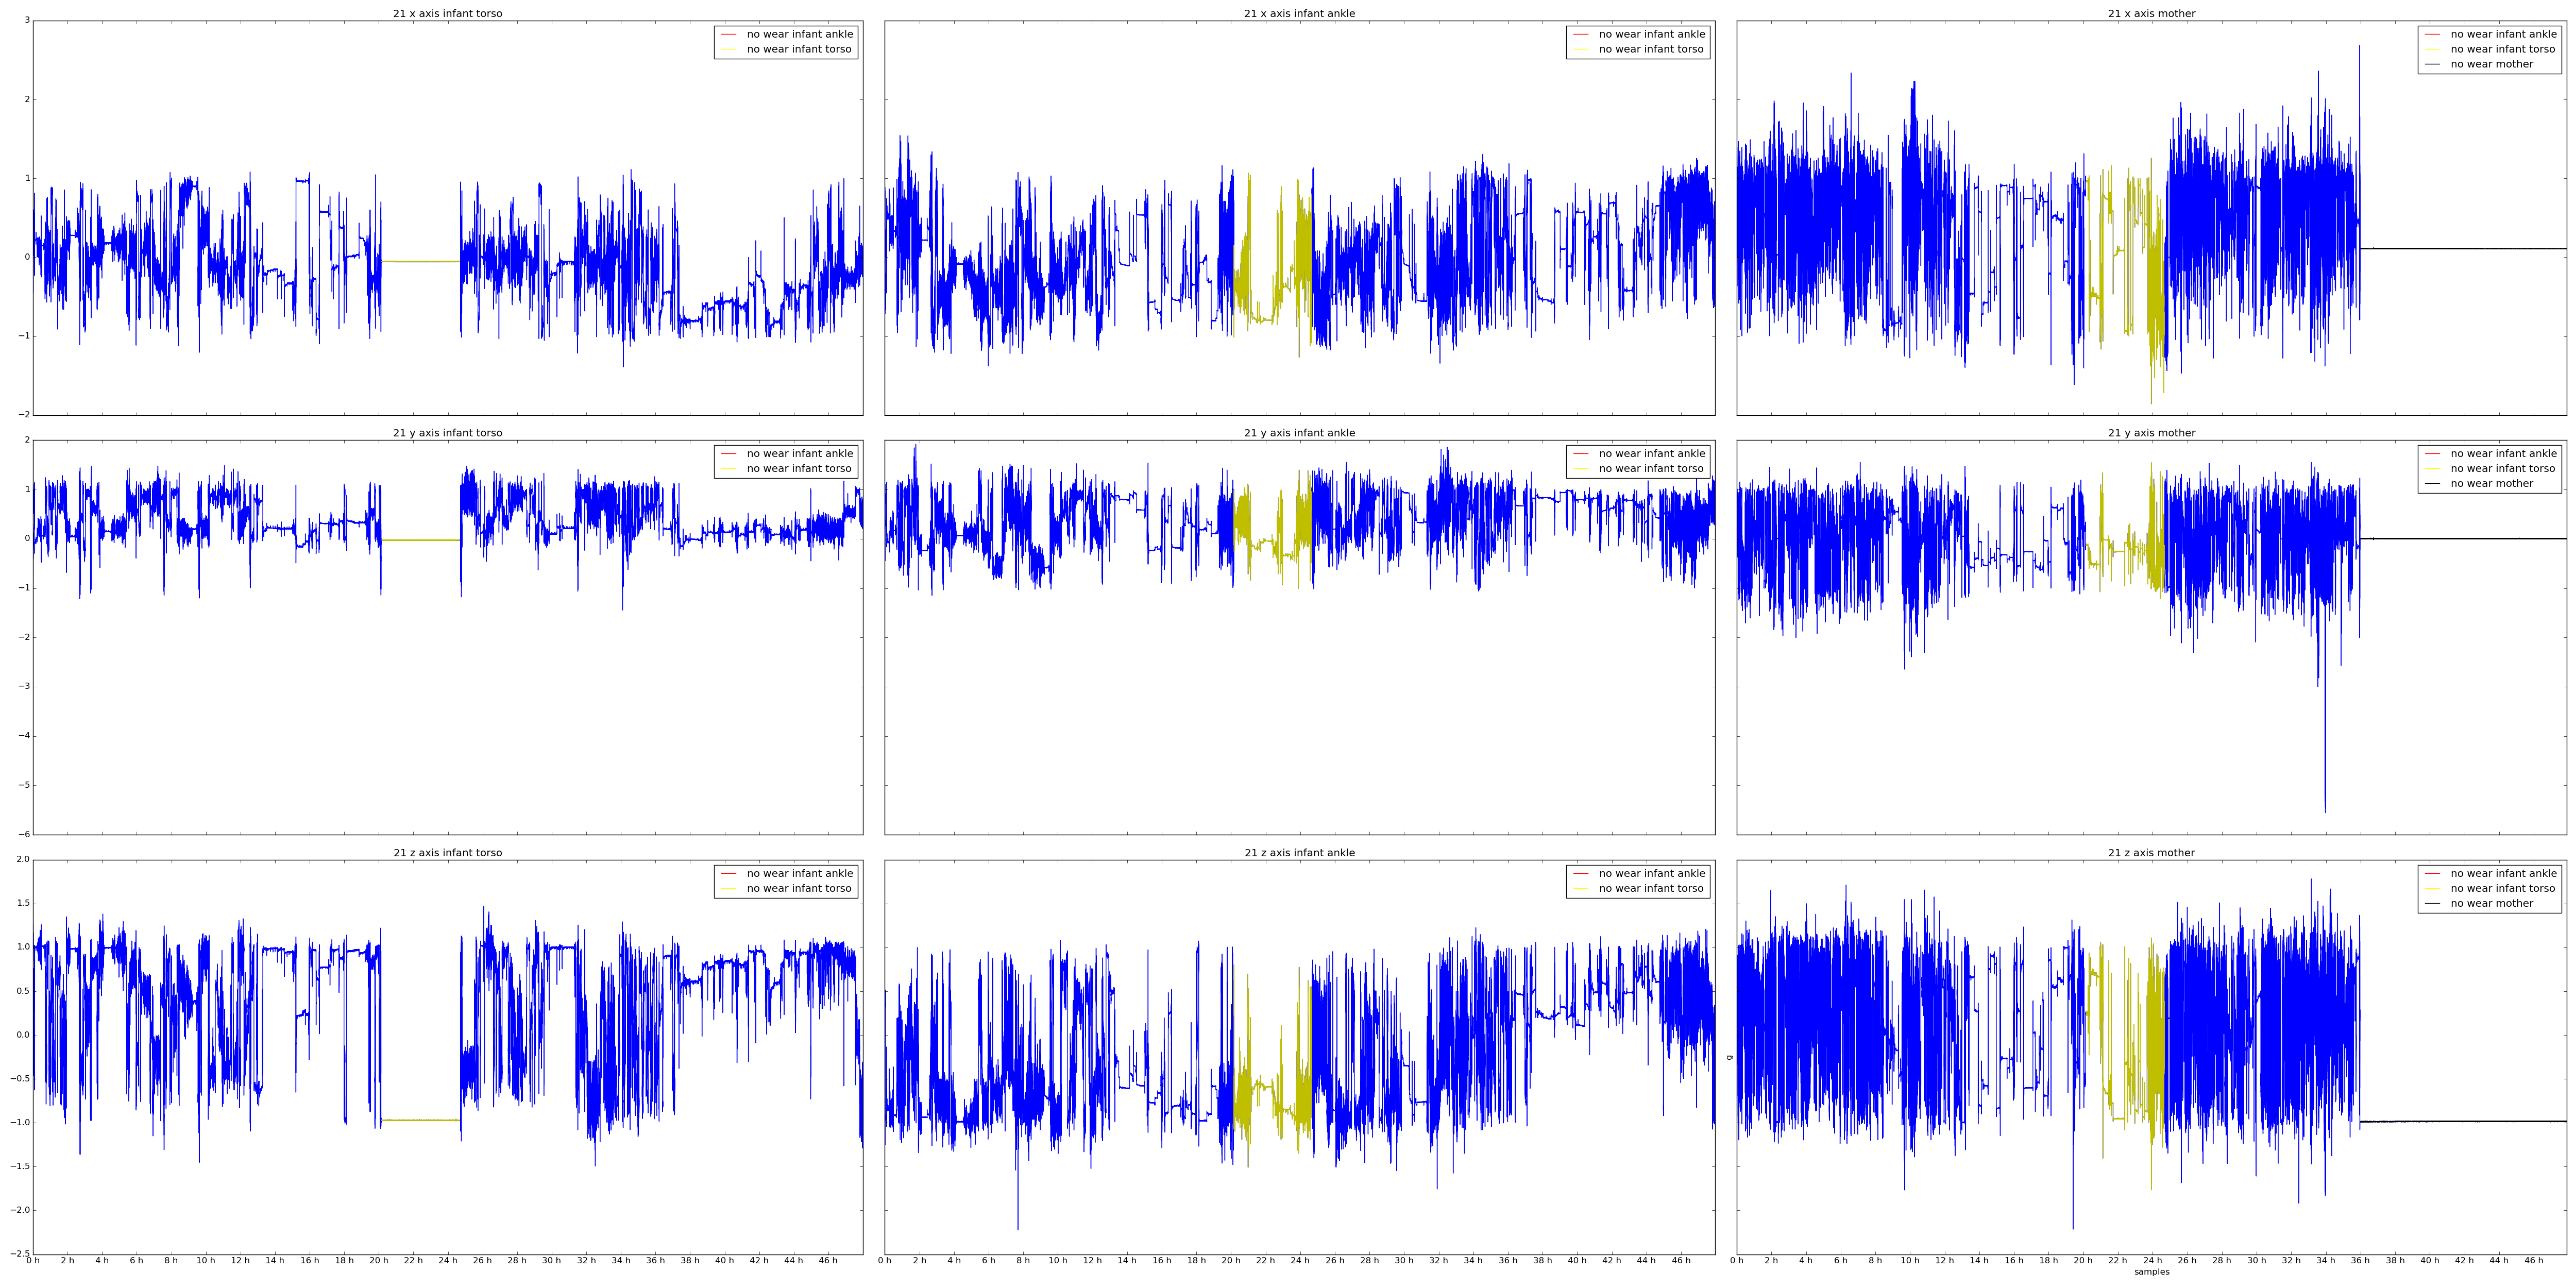
\includegraphics[width=15cm, height=8cm]{21NoWearTimeLabeled.png}
\caption{Example of accelerometer data for one infant-mother pair. The x, y and z axis are aligned vertically, while the infant torso, infant ankle and mother wrist monitors are aligned horizontally. The yellow color represents infant torso non-wear time, which is subsequently colored in the rest of the measurements and the black color represents maternal non-wear time, which is colored only in maternal measurement.}
\end{figure}
\\
\subsection{Summary measure extraction}
Accelerometers can be designed to measure acceleration on a single axis, dual axes or three axes along with different sampling rates. For the accelerometer used in this project  (GENEA), it had been shown that sampling frequencies larger than 10 Hz and/or more than one axis did not significantly increase classification accuracy, when classifying 10-12 semistructured activities performed in the laboratory or an outdoor environment, while wearing the accelerometer on the right wrist[7]. As for the PA extraction step, the same requirements for accuracy should be justifiable, but when considering detection and extraction of accelerations due to the infant being moved, it might be useful to analyze data in each of the three axes separately. However, without training data available, the key information regarding the way accelerations are detected in the three axes, when the infant is being moved, is unknown. In this project, the accelerations contributed by the caretaker had to be therefor detected and corrected based solely on the data from the two monitors worn by the infant. The way the ankle and torso monitors were placed, the three axes of the two monitors were not aligned and with the mobility of the infants ankle they were liable to rotations. This presents a problem when one wants to compare the two outputs, since each of the axes should be aligned prior to the analysis. For the reasons given above, a summary measure over all three axes was derived. The summary of all three axes was derived by ,
POPRAVIT Z NOVIMI PODATKI



 which represented the output summarized over all three axes along with filtering and averaging.
The summary measure was calculated in Matlab by subtracting one from the averaged Euclidean norm of the three axes which were filtered with a median filter in a similar way as done in previous analysis[2], since it had been shown, that having more complicated summaries does not significantly improve the final extraction of PA[3]. The width of the median filter was 11 and its purpose was to remove any spikes from the measurement which are due to noise. The resulting Euclidean norm minus one was averaged over 0.2 seconds to further smooth the data and minimize the contribution of noise. When plotting the resulting summary measure for torso and ankle, one can  clearly see the substantial similarities in the measurements due to the caretakers contributions, example in Figure 2. 


\begin{figure}[h]
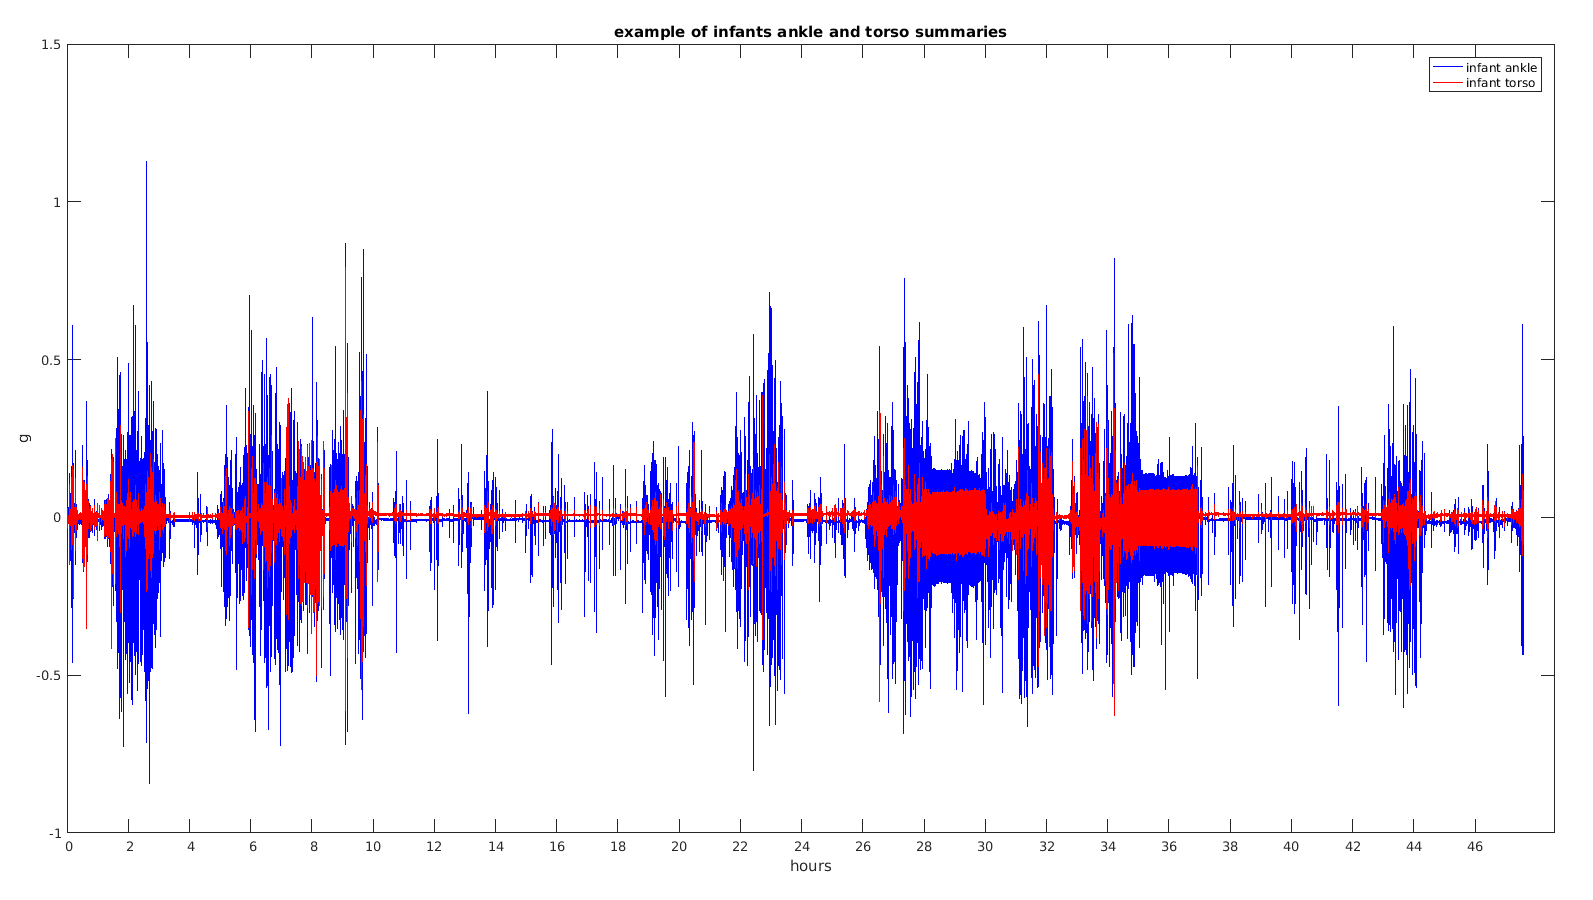
\includegraphics[width=15cm, height=8cm]{exampleTorsoAnkle.png}
\caption{An example of the derived summaries over all three axes for infant torso and infant ankle measurement, illustrating the degree of similarity in activity patterns, with visible leftovers of the gravitational acceleration.}
\end{figure}
\\
While the infant torso and ankle derived summaries show substantial similarity, the corresponding derived summary, of the maternal accelerometer data, only exhibits the same pattern of activity as the infant during the night, indicating plausible interaction between the mother and her infant, example in Figure 3.\\
\begin{figure}[h]
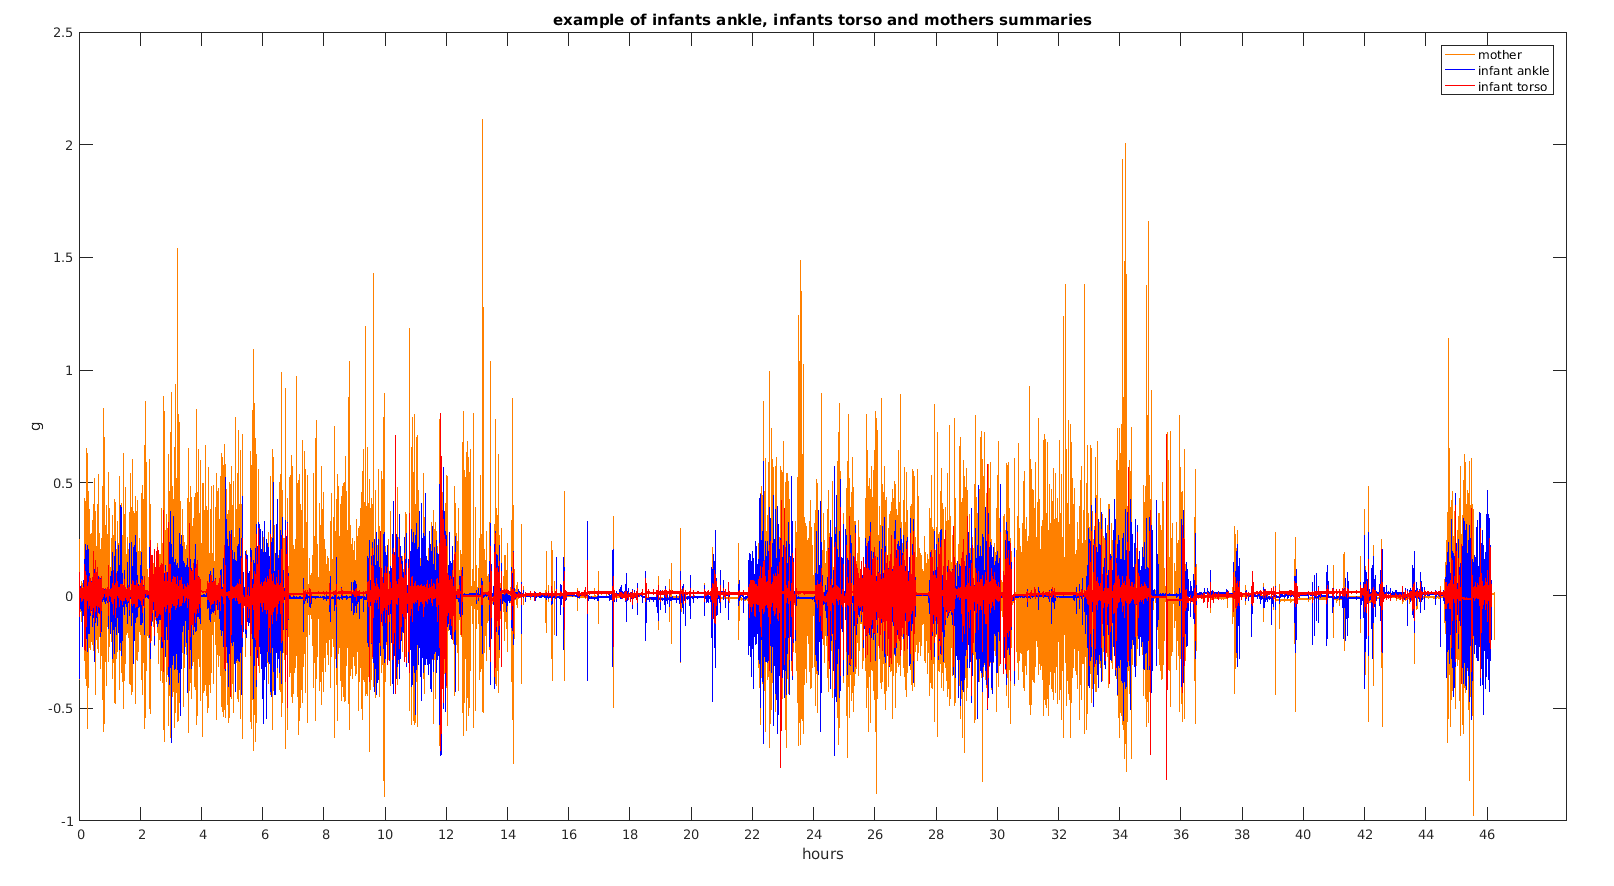
\includegraphics[width=15cm, height=9cm]{exampleTorsoAnkle2.png}
\caption{An example of the derived summaries of infant ankle, infant torso and maternal wrist measurements, illustrating the degree of similarity in activity patterns across night and day, with visible leftovers of the gravitational acceleration.}
\end{figure}

In Figure 2 and 3 one can observe the remaining baseline shifts due to leftovers of the gravitational accelerations that need further removal, which is discussed in the next subsection. 
POPRAVIT Z NOVIMI PODATKI
\subsection{Correcting for the gravity component}
The separation and removal of the gravitational component becomes more complicated when rotations are present in the measurement[3]. This can result in less accurate further processing, especially when outcomes from different monitors have to be compared. To ensure that the measurement does not reflect the influence of gravitation, the measurement baseline can be corrected to zero. Baseline correction is implemented in Matlab based on a smoothing method with penalized least squares[4]. The method is an extension of the Whittakers method for smoothing, which works by minimizing the following sum: 
\begin{equation}
S=\sum_{i} (y_i - z_i)^2  +  \lambda\sum_{i} (z_i - 2z_{i-1} + z_{i-2})^2\thinspace \thinspace ,
\end{equation}
where \textit{y} is the input signal, \textit{z} is the final smoothed signal and \textit{i} goes through the data points.
The first part of the sum ensures the best approximation of the input signal, while the second part represents the penalty for non-smoothness. 
In practice $\lambda$ is set from $ 10^{2} \leq \lambda \leq 10^{9}$ and its value depends on the input data and the desired final result. Since the goal of the baseline correction in the project was to keep all the amplitudes intact, but only correct the rough baseline, $\lambda$ is set to $10^{9}$.
\\
Reformatting the above into a linear system of equations, we get:

\begin{equation}
(I + \lambda D'D)z = y\thinspace \thinspace ,
\end{equation}

where I is the identity matrix and D is its differential matrix. 
The computational time and space can be optimized, using sparse matrices and Cholesky factorization. The resulted over-smoothed signal represents the baseline and is therefor subtracted from the measurement. This way, the amplitudes remain intact, but the baseline drifts and jumps are removed and the signal baseline is set to zero, example Figure 4. 

\begin{figure}[h]
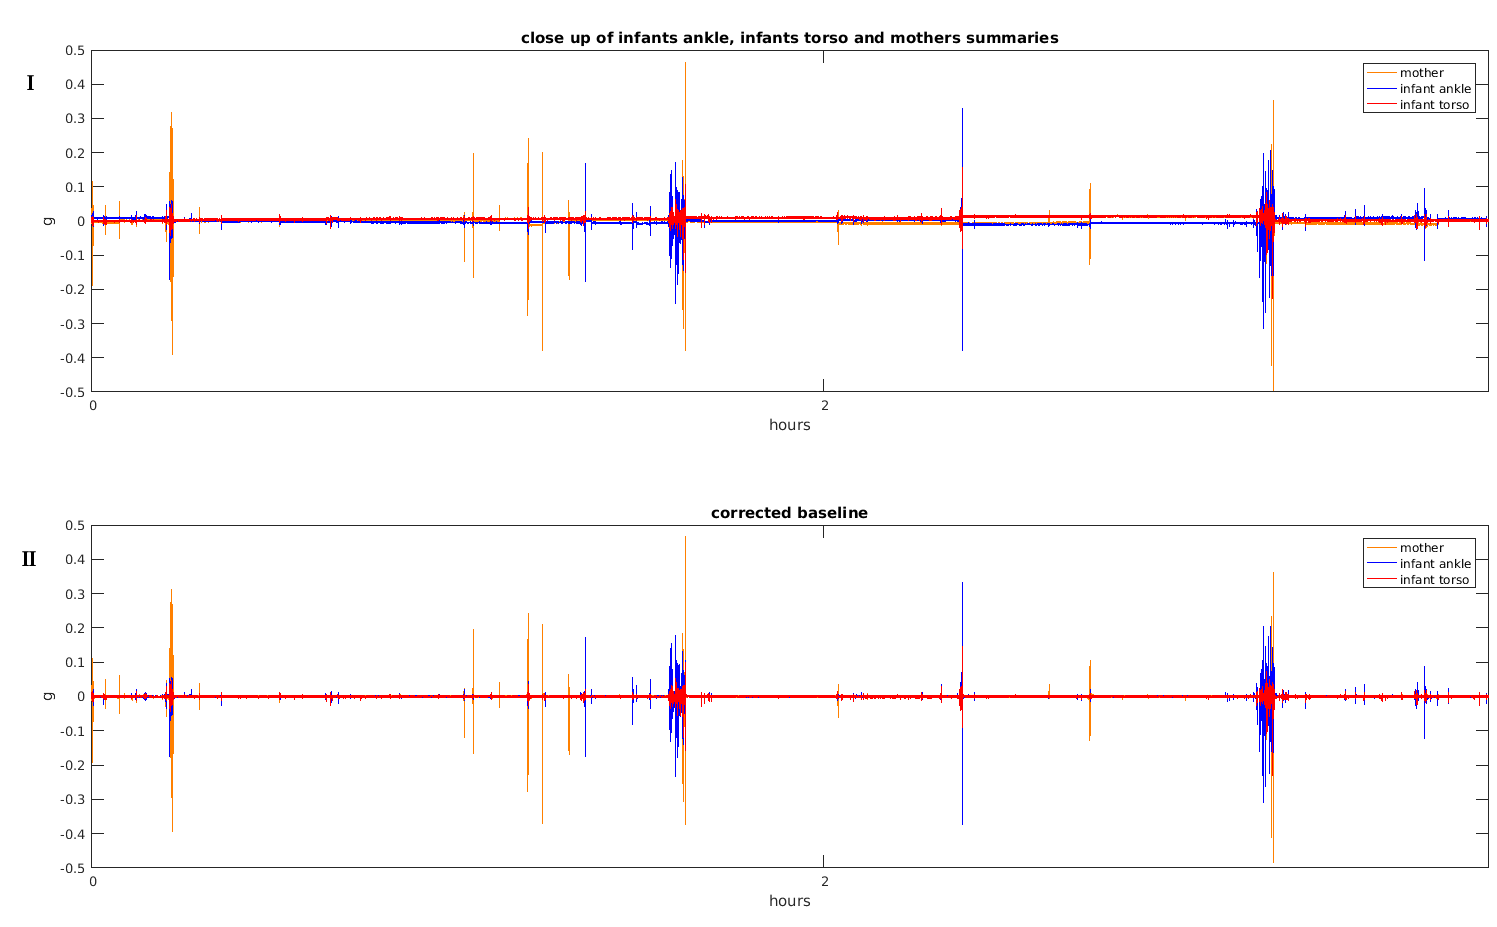
\includegraphics[width=15cm, height=10cm]{exampleTorsoAnkle5.png}
\caption{A close up of all three derived summaries for infant torso, infant ankle and maternal wrist accelerometer data, before and after the baseline correction.}
\end{figure}
\subsection{Accelerations contributed by the caretakers}
The accelerometer is liable to pick up any acceleration caused by the subject moving, regardless if the subject is in PA or is being moved by another person. Infants at 4 month old age are completely dependent on the caretaker. Besides the basic tasks like feeding, bathing, dressing, etc., the infants at 4 months require a substantial amount of carrying, placing and cradling. This results in significant contributions of accelerations caused by the person caring for the infant. In 2009 a paper titled \textit{Mechanical Measurement of Infant Activity: A Cautionary Note}[1] was published. The main message of the paper was that much of infants measured activity may be confounded by their caretakers contributions. An experiment was performed as a basis for the paper, where a mother and her 3 month old infant had a normal 24 hour day with usual activities, while a researcher with a motionless doll would mimic everything the mother did with her infant. Both the infant and the doll wore motion loggers on the chest and ankle. The results were then analyzed and compared. As one would expect, the dolls measurement showed a substantial amount of activity which would normally be unusual for a motionless doll. When comparing infants activity levels to the ones of the doll, approximately 45\% more activity was detected, meaning that the monitor will pick up both, the infants and caretakers contributions. In 2014 a PhD thesis was submitted, titled \textit{Physical activity in infancy: assessment of an intervention to increase physical activity in infants}[6]. As part of the research, the defended studied and analyzed the feasibility to assess PA in 6-month old infants using an accelerometer, based on a validation study performed in 2012, with the results available in a conference abstract[5]. The goal of the study was to assess the degree of caregiver confounding that might be expected in these measurements. Similar to before[1], the infants and motionless dolls wore three accelerometers, one on the wrist, one on the ankle and one on the waist. While the caretaker would perform several activities with the infant, the research assistant would mimic their actions with the doll. Overall 34 mother-infant pairs participated, although some did not perform all the activities. The results showed that when the infant is pushed in a stroller, 29\% of the arm movement and 9\% of the leg movement is due to contributing accelerations, while when being carried, contributing accelerations add up to 23\% of the arm movement and 52\% of the leg movement. With another type of activity with a Swiss ball, 28\% of the arm movement and 21\% of the leg movement was due to contributing accelerations. For all activities, the waist accelerometer recorded more activity on the doll rather then the infant, which resulted in an invalid measurement. An interesting observation showed that the overall output differed significantly between the three differently placed accelerometers, when in fact recording the \textit{same} activity. Overall, the study[5] showed that up to half of the detected activity can be due to contributing accelerations, while these contributions differ significantly between the activities performed and between the differently placed monitors, as well as between the caretakers.\\
The overall variability presents a potential problem as it is currently still unexplained, making modeling of such data impaired. In the current project, the two monitors were placed on different body parts of the infant, as well as on the mothers wrist, to enable correction due to contributing accelerations. But when the two monitors have different outcomes for the same activity and the variability between the subjects is high, the correction becomes complicated. This is even further complicated by the fact that a monitor placed on infants torso is liable to record accelerations that are not due to infant being moved and are therefor not recorded on the ankle monitor, even though the infants at 4 month are not able to move their torso. It had been shown that the movement of the chest while breathing has an amplitude of 10 mg, while heart beating will result in an amplitude of 80 mg[8]. With such sensitivity, infants crying and flexing, along with limb movement should also be picked up by the torso monitor.\\ Such issues raise doubt that a simple subtraction of the torso placed measurement from the ankle placed measurement will result in a valid and useful outcome and several more advanced and complicated approaches were designed and tested for this reason. Total, these approaches were tested:
\begin{itemize}
\item \textbf{A.} Simple subtraction of measurements
\item \textbf{B.} Subtraction of windowed intensities
\item \textbf{C.} Correction based on windowed intensities
\item \textbf{D.} Correction based on correlated windowed intensities
\item \textbf{E.} Complete removal of blocks where infant was moved
\end{itemize}
Prior all approaches, apparent blocks of \textit{infant being moved} were detected, based on the substantially increased SD in both, torso and ankle placed measurement. This approximation was used to asses the different results from the different approaches. Blocks of \textit{infant being moved} were detected similar as in non-wear detection. Example of these blocks noted in both measurements in Figure 5.
\begin{figure}[h]
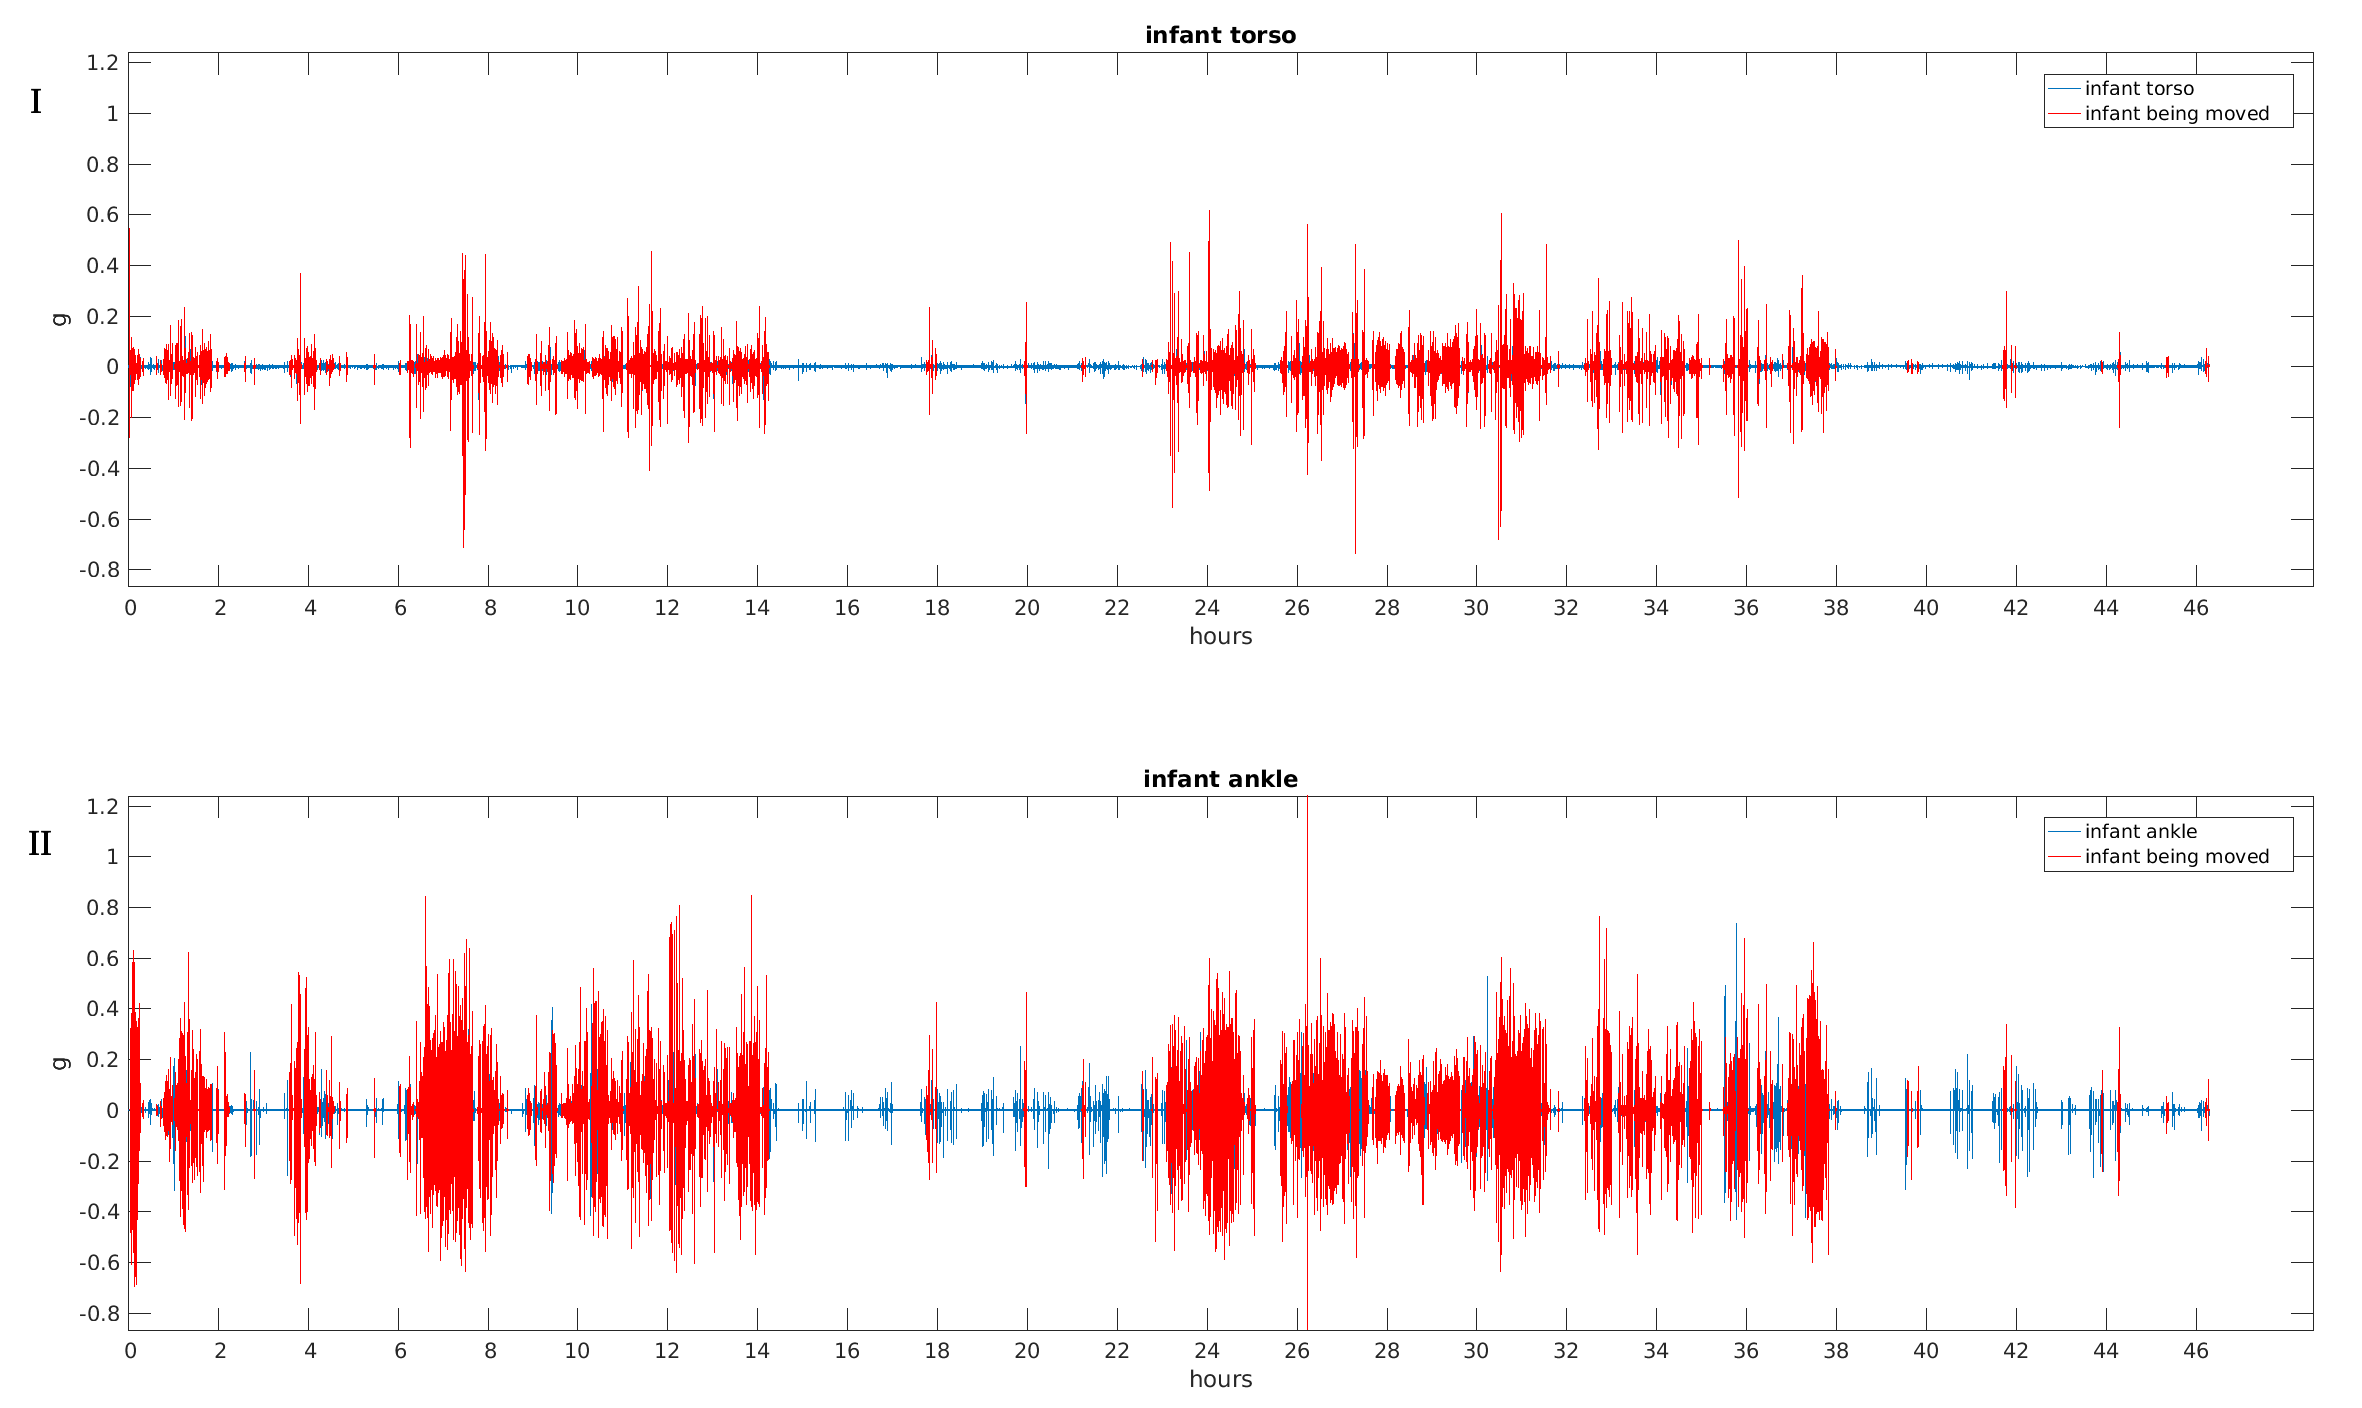
\includegraphics[width=15cm, height=8cm]{final_plotE.png}
\caption{Example of the torso and ankle placed measurements, where blocks of \textit{infant being moved} are noted with red.}
\end{figure}
\\\\Based on these blocks, several variables were calculated. The overall proportion of time the infant was being moved and frequency of infant being moved, along with eight more detailed variables. Detailed variables are proportions of time in combining short and long duration with low and high intensity blocks along with the frequency. Overall, infants were being moved by another person on average 35.0\% of the time, with minimum at 21.0\%, maximum at 45.4\% and SD 5.9\%. 
\\As predicted, \textbf{A} did not give promising results, as the point to point difference was too significant, even though the measurements were summarized, filtered and averaged and showed substantial similarities on a large scale. Simple subtraction in fact amplified the contributing accelerations, as the average SD in the apparent blocks of \textit{infant being moved} increased by an average of 15.0\% while the average absolute intensity increased by average 20.5\%. Example of torso and ankle placed measurements and the result from simple subtraction in Figure 6. Even when averaging the measurement over 1 second, instead of 0.2, the average SD still increased by average 14.9\% and the average intensity by average 18.3\%.
\begin{figure}[h]
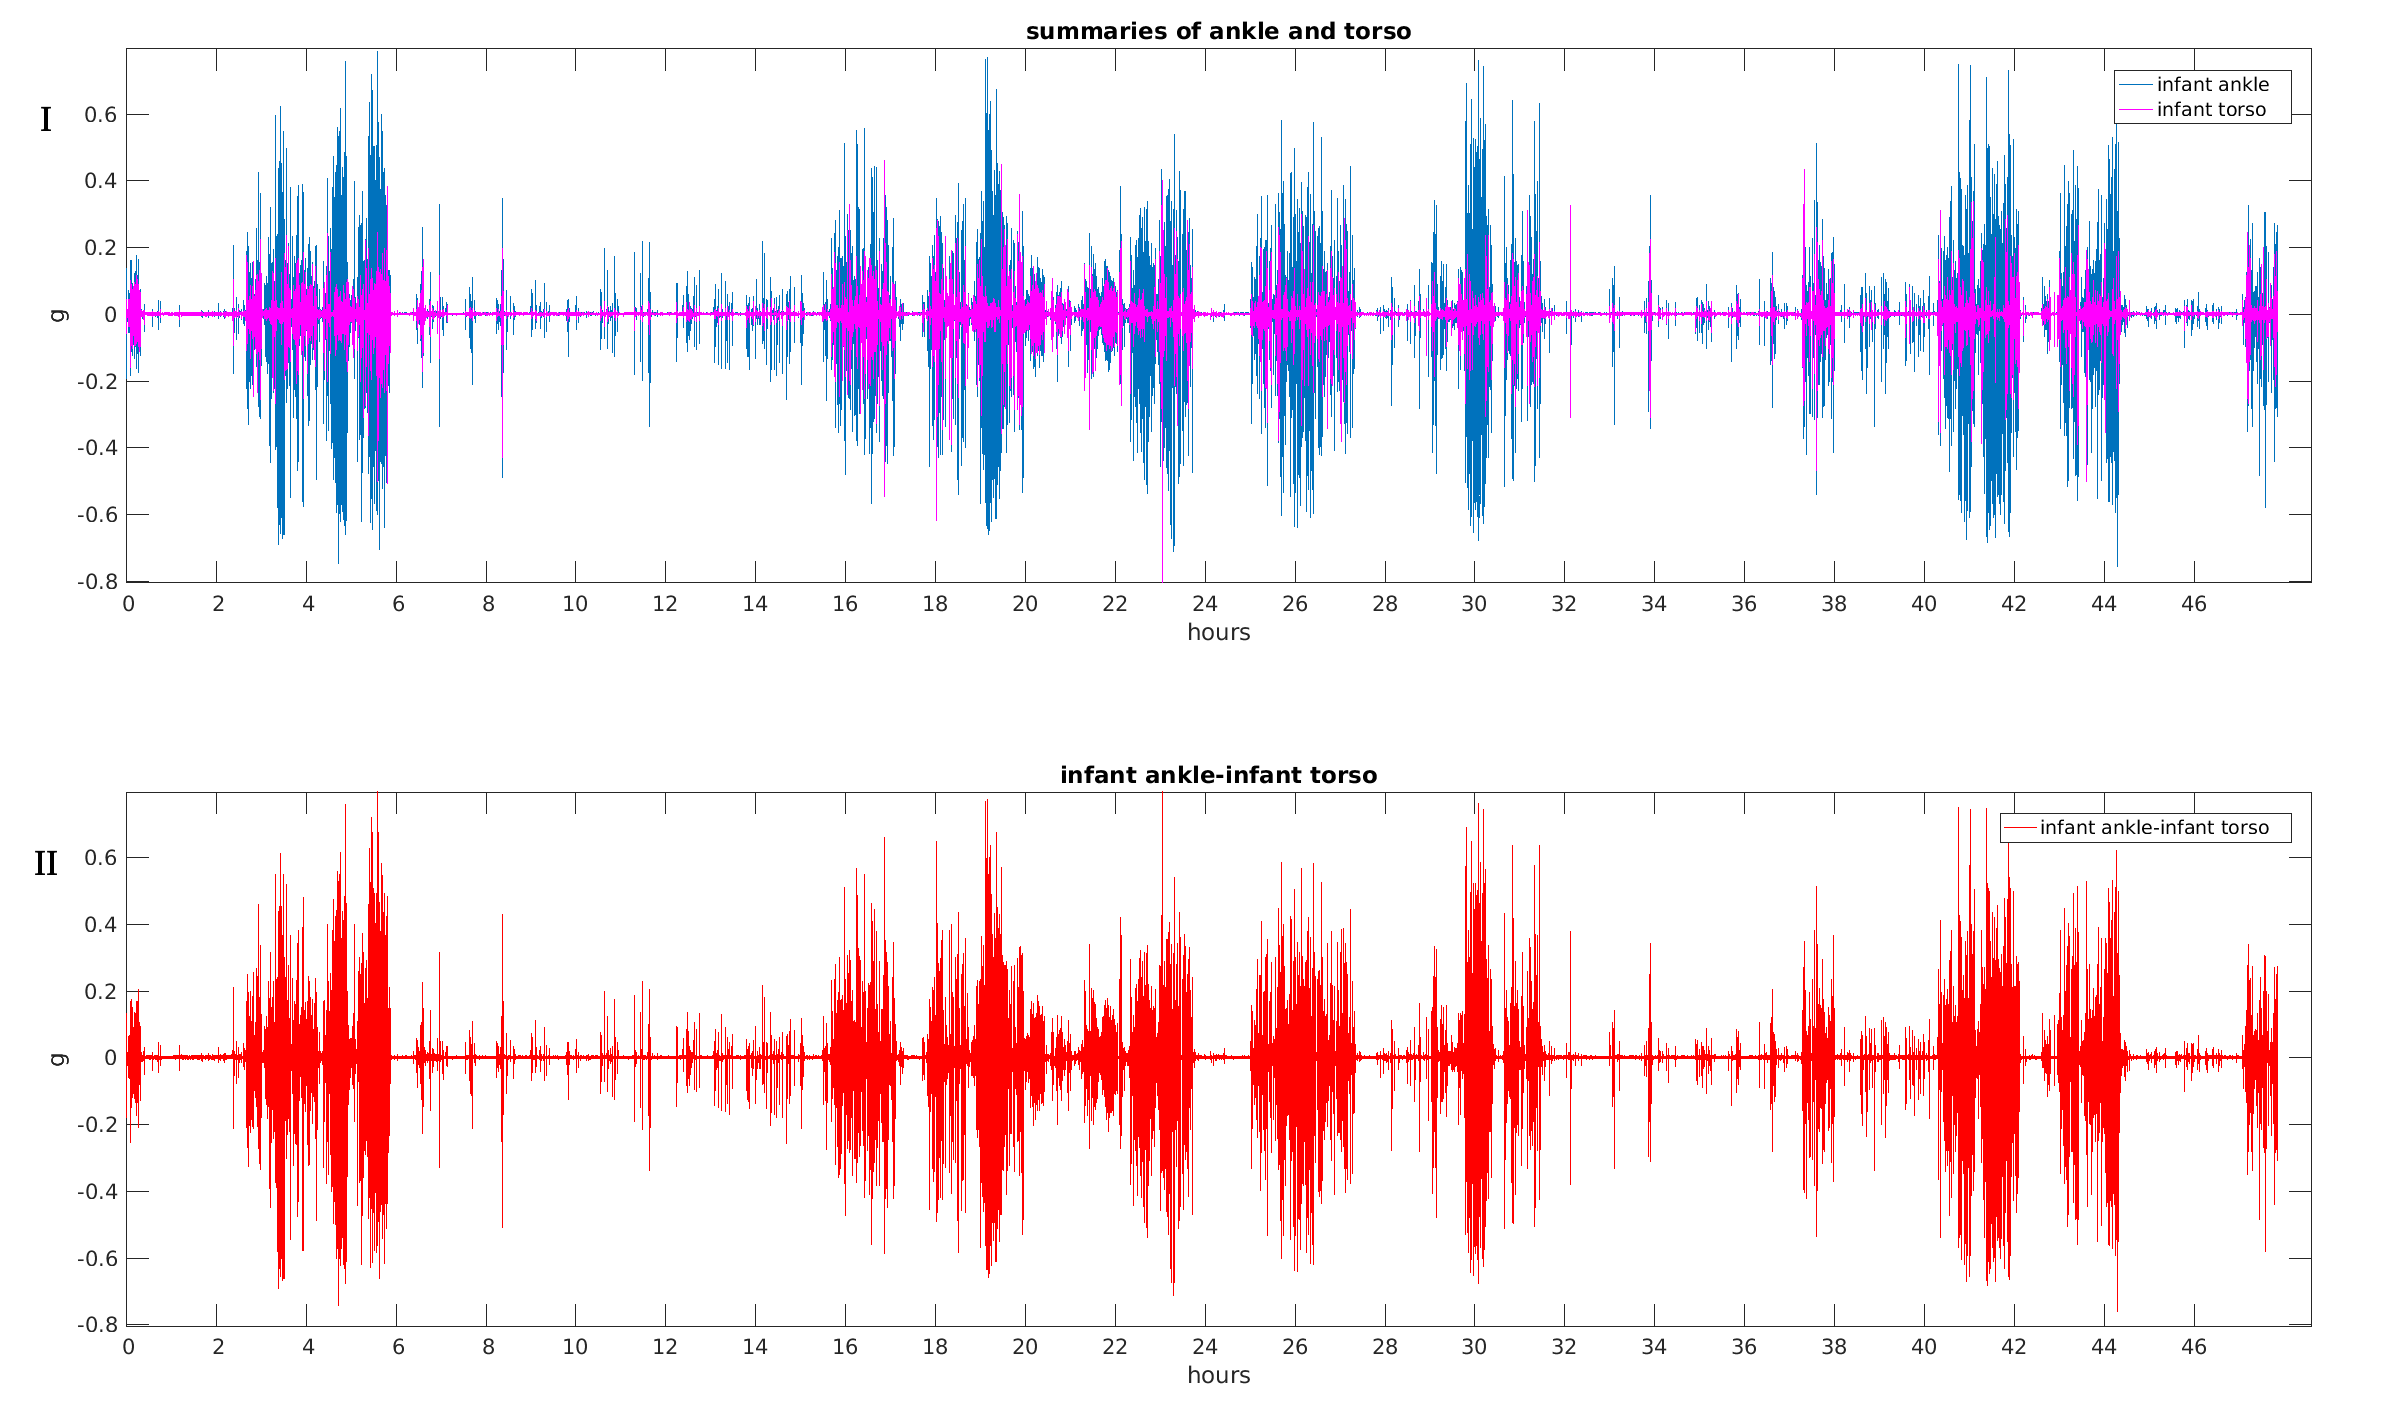
\includegraphics[width=15cm, height=8cm]{SimpleSubtracting.png}
\caption{A plot exhibiting the result of a simple subtraction of the torso placed measurement from the ankle placed measurement.}
\end{figure}
\\As the measurements exhibit a substantial amount of similarity on a large scale, but seem to be too different point to point, the second and third approaches, \textbf{B} and \textbf{C} use an even more summarized measure and its features, to either do a simple subtraction or a correction. The process is implemented in Matlab. Both, torso placed and ankle placed measurements are windowed in a loop over 1 minute long windows, which corresponds to 2400 points. For each window, the absolute intensity of each monitor is calculated as the sum of absolute values, divided with the window length. In approach \textbf{B}, the torso intensity is simply subtracted from the ankle intensity and the final result is an even further summarized ankle placed measurement with torso intensities subtracted, example in Figure 7.
\begin{figure}[h]
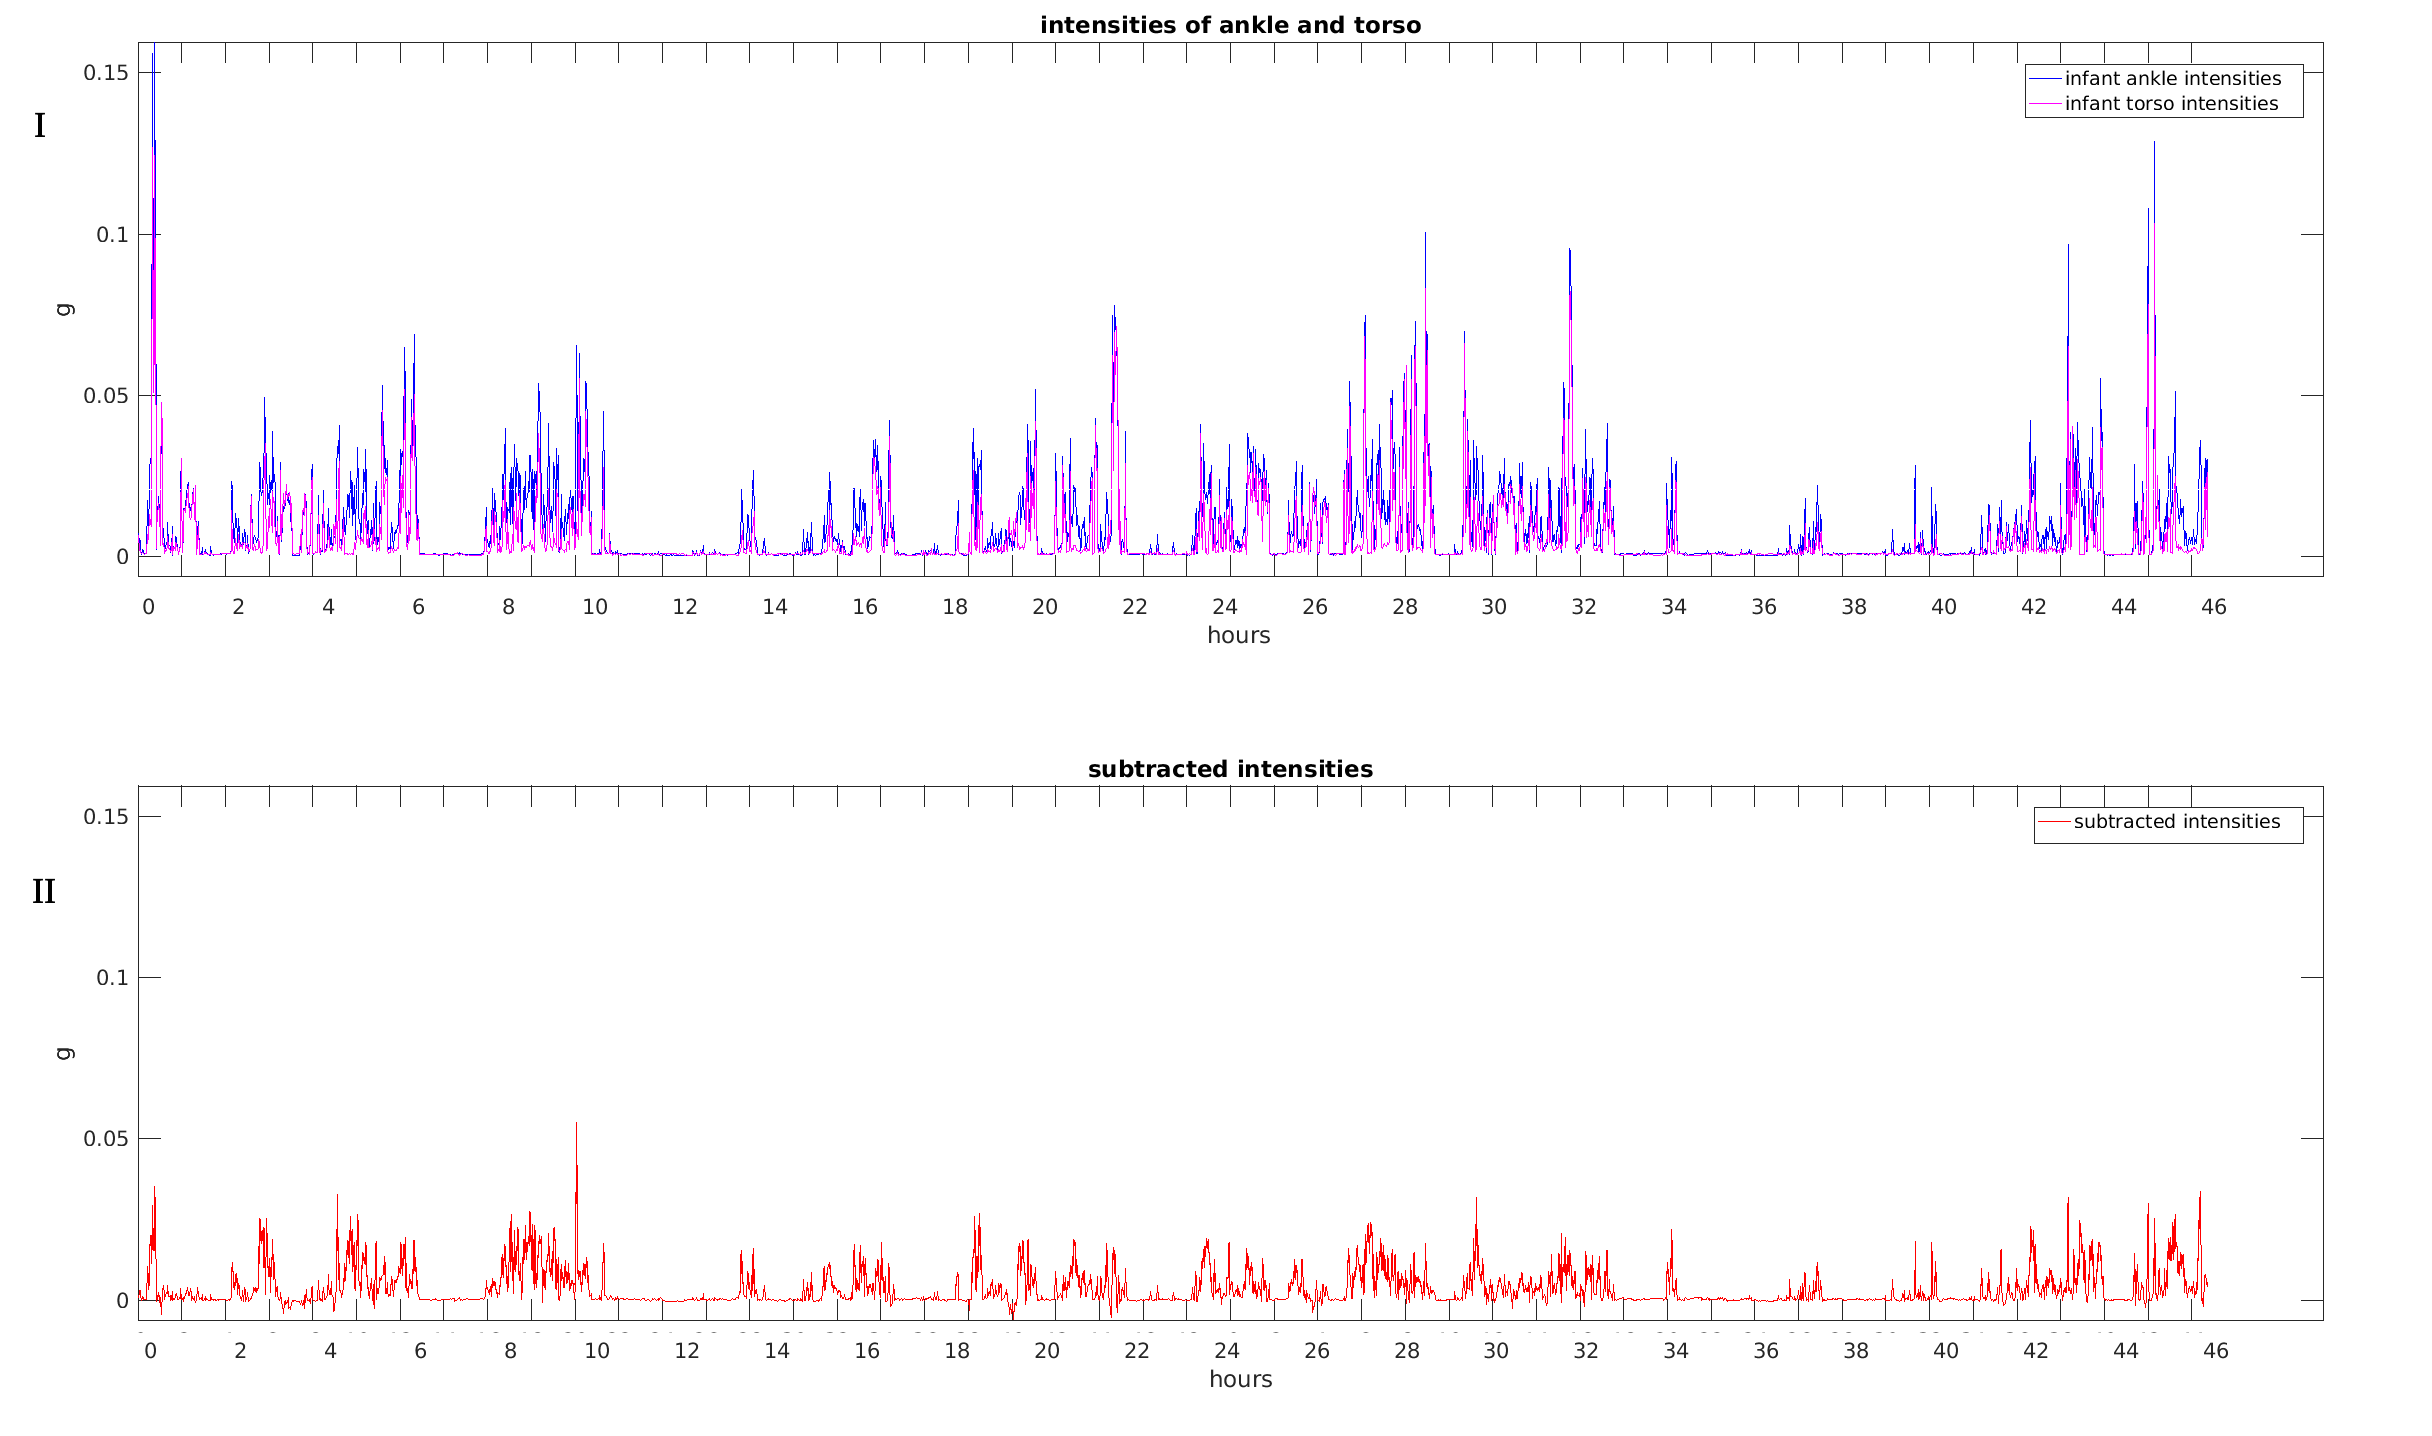
\includegraphics[width=15cm, height=6.5cm]{subtractedIntensities.png}
\caption{A plot exhibiting the result of subtracting the windowed intensities of the torso placed measurement from the ankle placed measurement.}
\end{figure}
\\
In the approach \textbf{C}, the ratio between the ankle intensity and torso intensity in each window is used to reduce each point in the ankle measurement in the corresponding widow. For example, if the torso intensity is half the ankle intensity, all the points in the window are reduced for half of their size, example in Figure 8.
\begin{figure}[h]
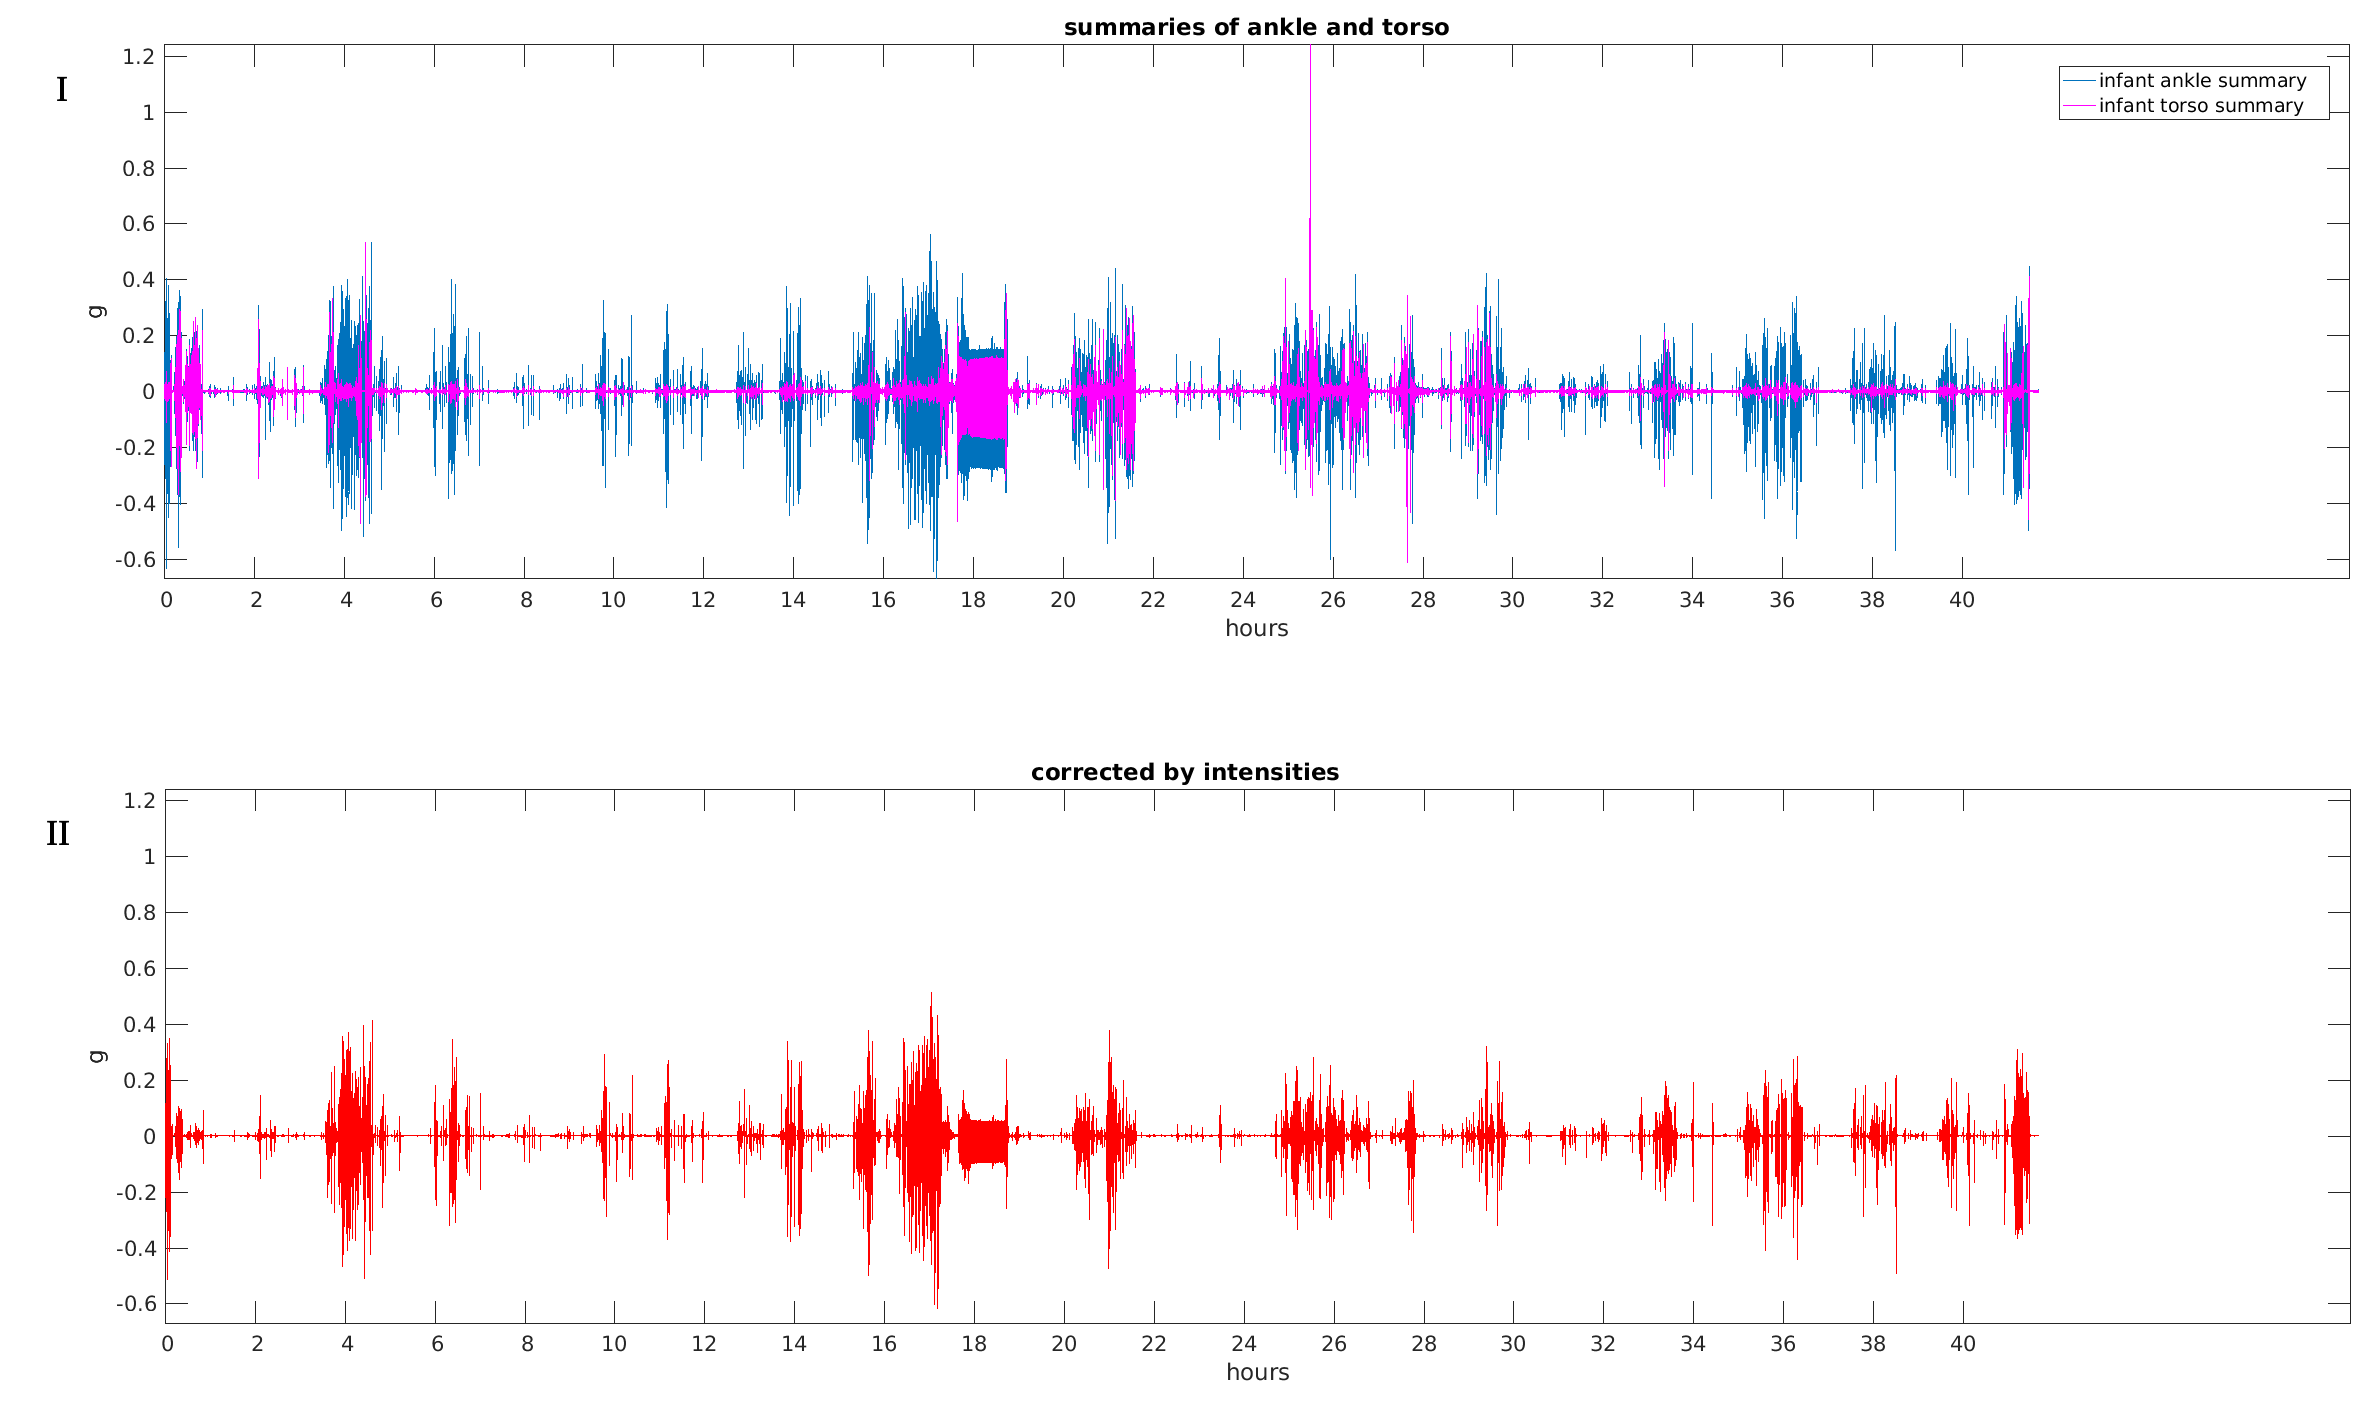
\includegraphics[width=15cm, height=6.5cm]{correctingIntensities.png}
\caption{A plot exhibiting the result of correcting the ankle placed measurement based on the ratio between the windowed intensities.}
\end{figure}
\\
In both approaches, the measurement is even further summarized and again the parameter representing the length of the window influences the final result. Short windows might preserve the local differences between the two monitors, while long windows might over summarize the data, especially if used further for PA extraction. Since training data is not present, such parameters have to be set by trial and examination, which is time consuming and the quality of the result is subjective. \\
In approach \textbf{B}, the outcome used for future PA extraction is more summarized then in other approaches.
This could influence the result of the extraction, since PA detection is limited down to a summary of a minute which makes it less accurate. This is avoided in the approach \textbf{C}, which in compare to approach \textbf{A}, decreases the average SD and absolute intensity of the apparent \textit{infant being moved} blocks by average of 43.9\% and 47.3\% of the original SD and original intensities respectively. Although both approaches reduce SD and absolute intensity they do not completely correct the ankle placed measurement, as left overs of the contributing accelerations are clearly visible in both cases, while one can also observe negative intensities due to the fact that the torso placed monitor can obviously also record more intensive accelerations than the ankle placed one. Since it had been shown that the same activity performed by the caretaker with the infant is recorded differently by differently placed monitors, there should be a scaling factor involved when doing such subtractions or corrections. Obtaining such a scaling factor might be problematic, since it had also been shown that different activities result in different ratios between the differently placed monitors, as well as that there is a high variability between the subjects. Things get even more complicated if considering the fact that the two monitors will also pick up other accelerations, mainly infants own accelerations which are unique for that specific body part, like for example accelerations due to crying, breathing, heart beat or kicking. Without having a well defined training dataset it is difficult to tell which of the remaining accelerations left after approaches \textbf{B} and \textbf{C} are due to the excessive detection of contributing accelerations on the ankle placed monitor or due to infants PA. Nevertheless, the approaches can be improved. The overall concept of subtracting implies that the torso placed monitor will record accelerations equal or smaller then the ankle placed one, as well as that the degree of correction is dependent on the ratio of intensity instead of similarity. If similarity between the intensities is obtained, it can be used as an approximation of the true scaling factor needed to accurately correct the ankle placed monitor. \\
In the approach \textbf{D}, an attempt is made to obtain signal similarities based on the similarity of windowed intensities, using Pearsons correlation coefficient. The goal of the approach is to find similar patterns between the two measurements and then decrease the ankle placed measurement based on the degree of similarity. The idea behind this is that even though the two differently placed monitors might record the same activity different, there should be an underlying pattern in both, at least on a large enough window scale over the absolute intensities. For example some windows might exhibit similarity only in the rough changes as in Figure 9, while others might be more overall similar even on the local scale as in Figure 10.
\begin{figure}[h]
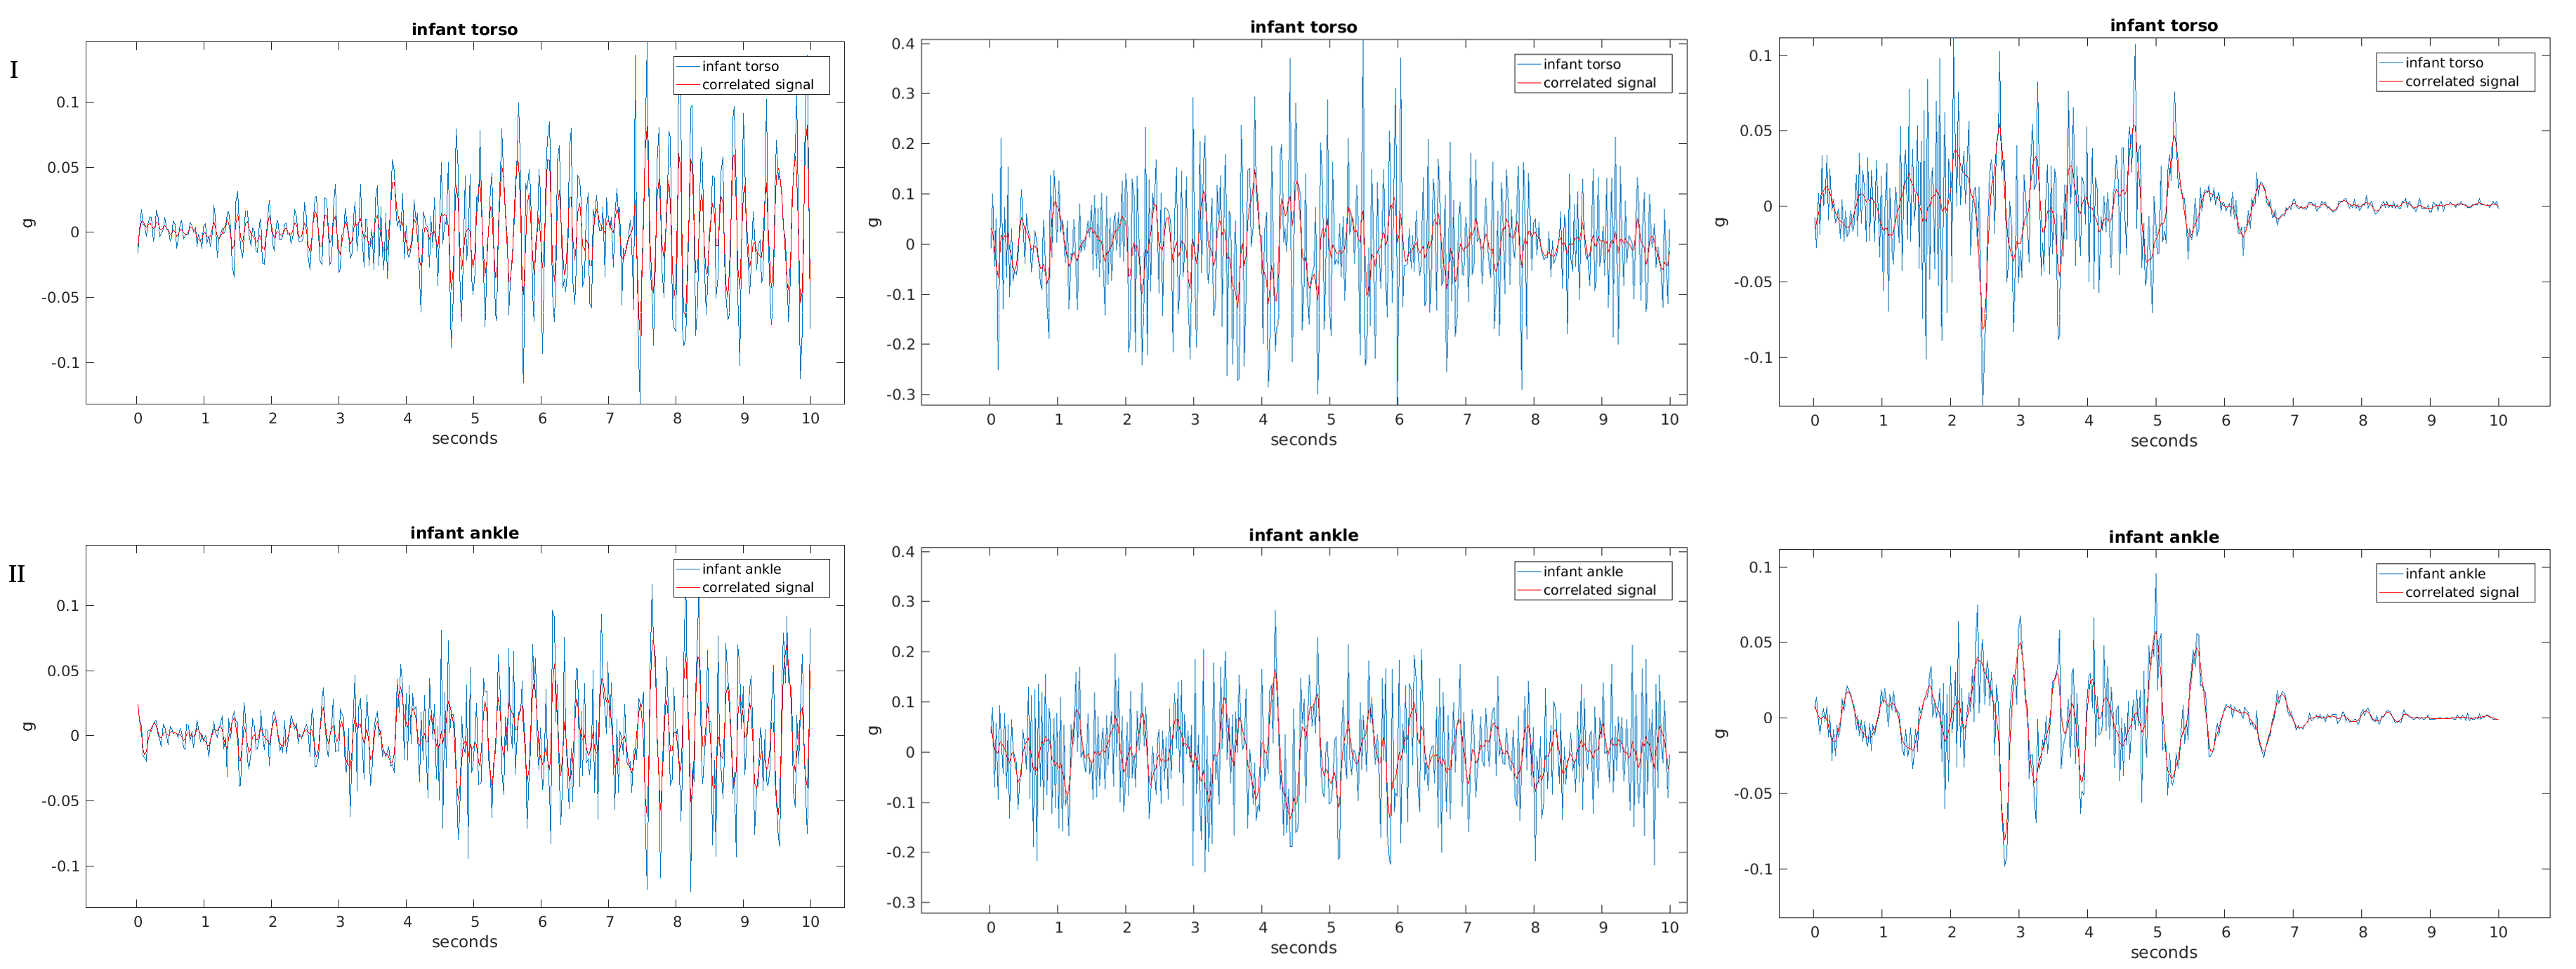
\includegraphics[width=15cm, height=6.5cm]{roughSimilar.png}
\caption{A plot showing a few examples of rough similarities between torso and ankle placed measurement.}
\end{figure}
\begin{figure}[h]
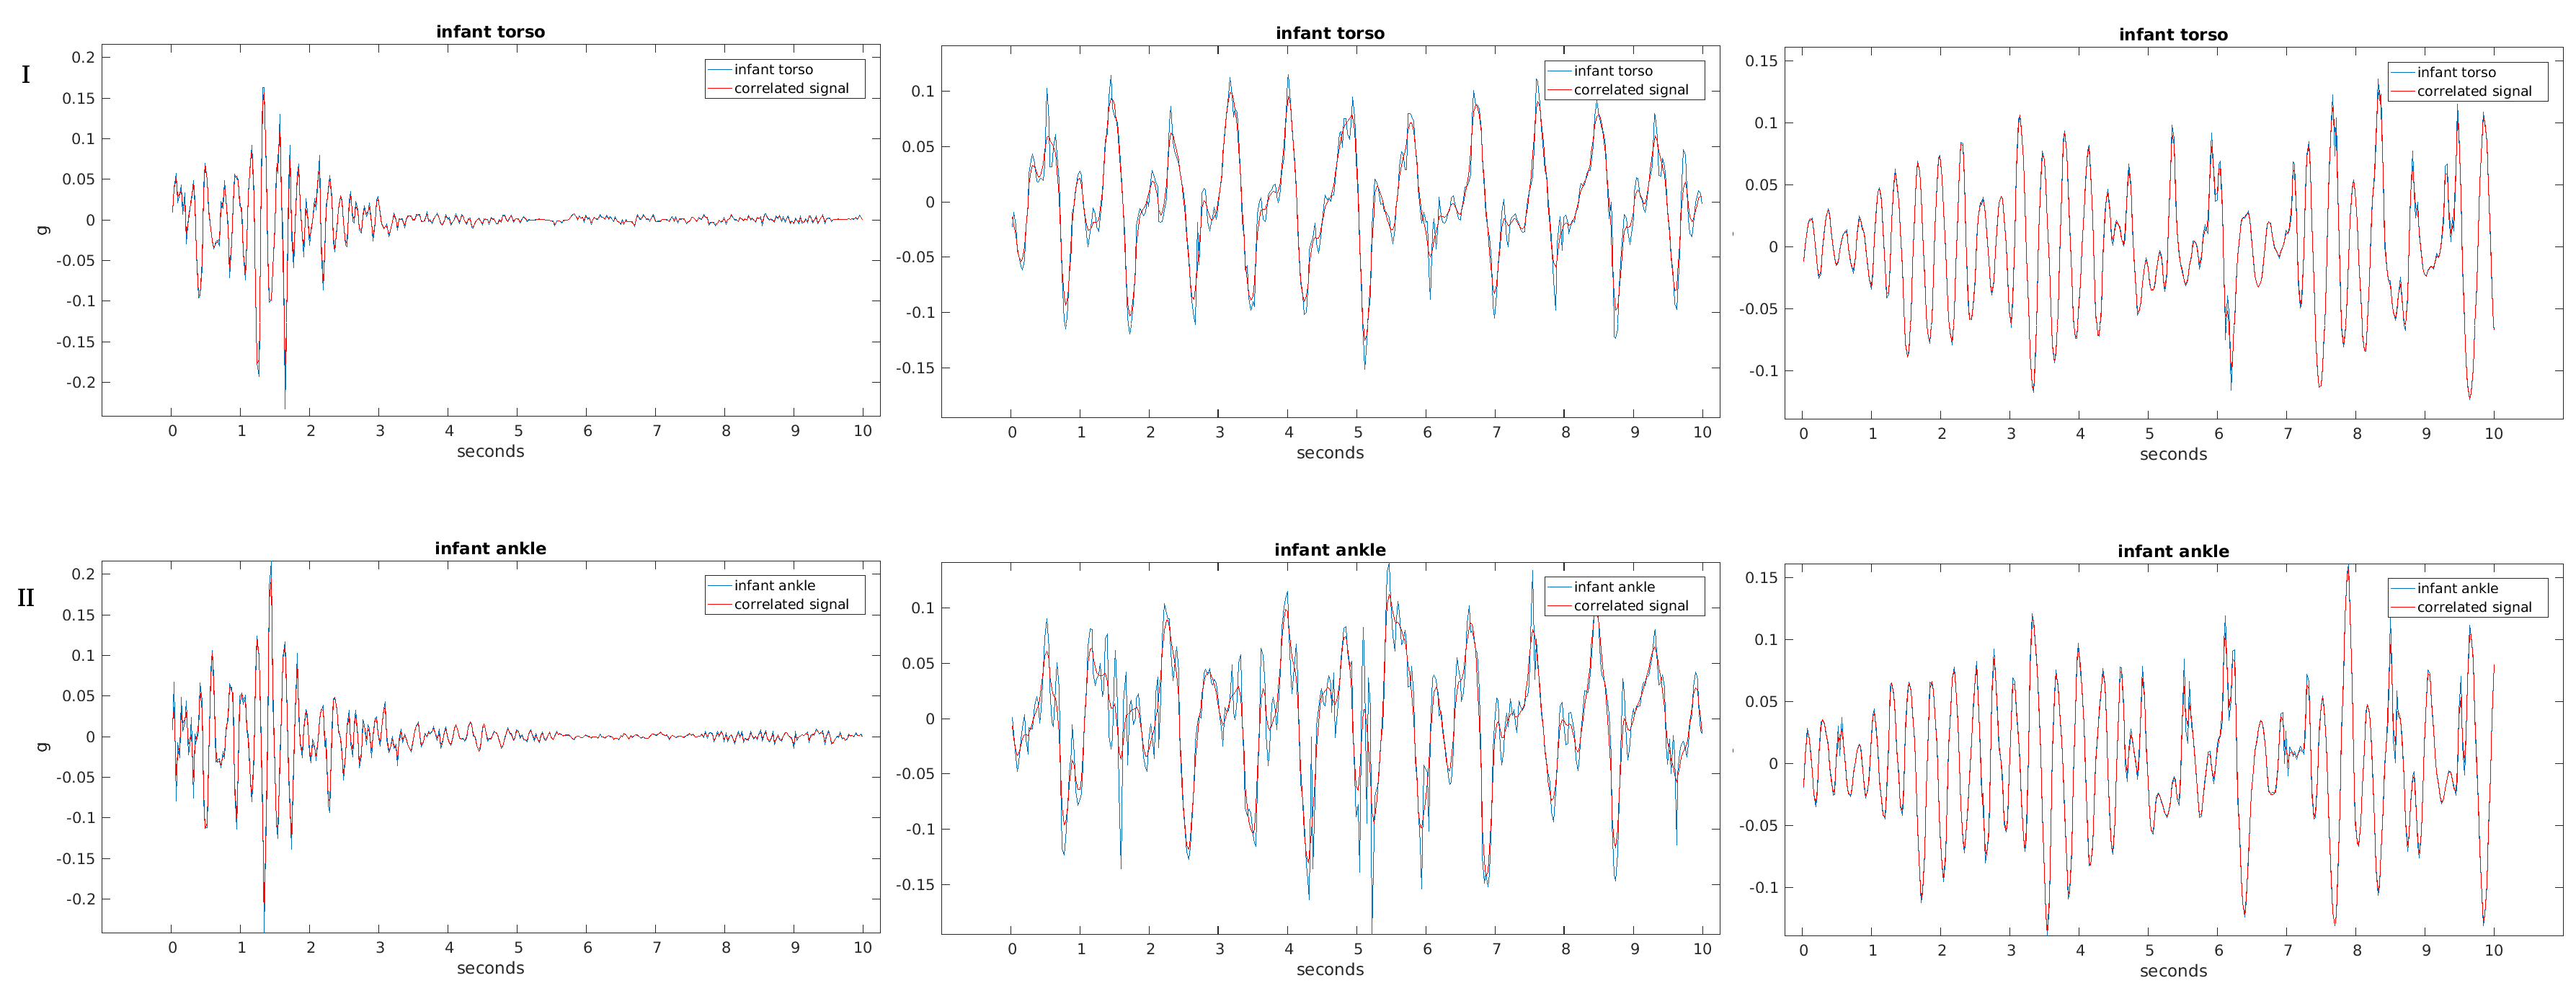
\includegraphics[width=15cm, height=6cm]{localSimilar.png}
\caption{A plot showing a few examples of precise similarities between torso and ankle placed measurement.}
\end{figure}
\\
The main issue with previous approaches \textbf{A}, \textbf{B} and \textbf{C} are the local point to point differences between the two differently placed monitors recording the same activity. These differences are in a form of larger intensities on one of the monitors, presence of other accelerations or noise in one or both monitors or in a form a time lag, examples in Figure 11.
Taking these differences into account, we would still like to determine if the two measurements in a given window are changing together due to being under the influence of the same activity, which is why calculating their covariance is of interest. Pearson correlation is obtained by dividing the covariance of the two variables by the product of their standard deviations and is a common correlation used for comparing signal similarities, especially in alignment[9]. The fact that it is invariant to separate changes in location and scale in the two variables being compared, gives it potential to expose the underlying similarities of the two differently placed monitors.
\begin{figure}[h]
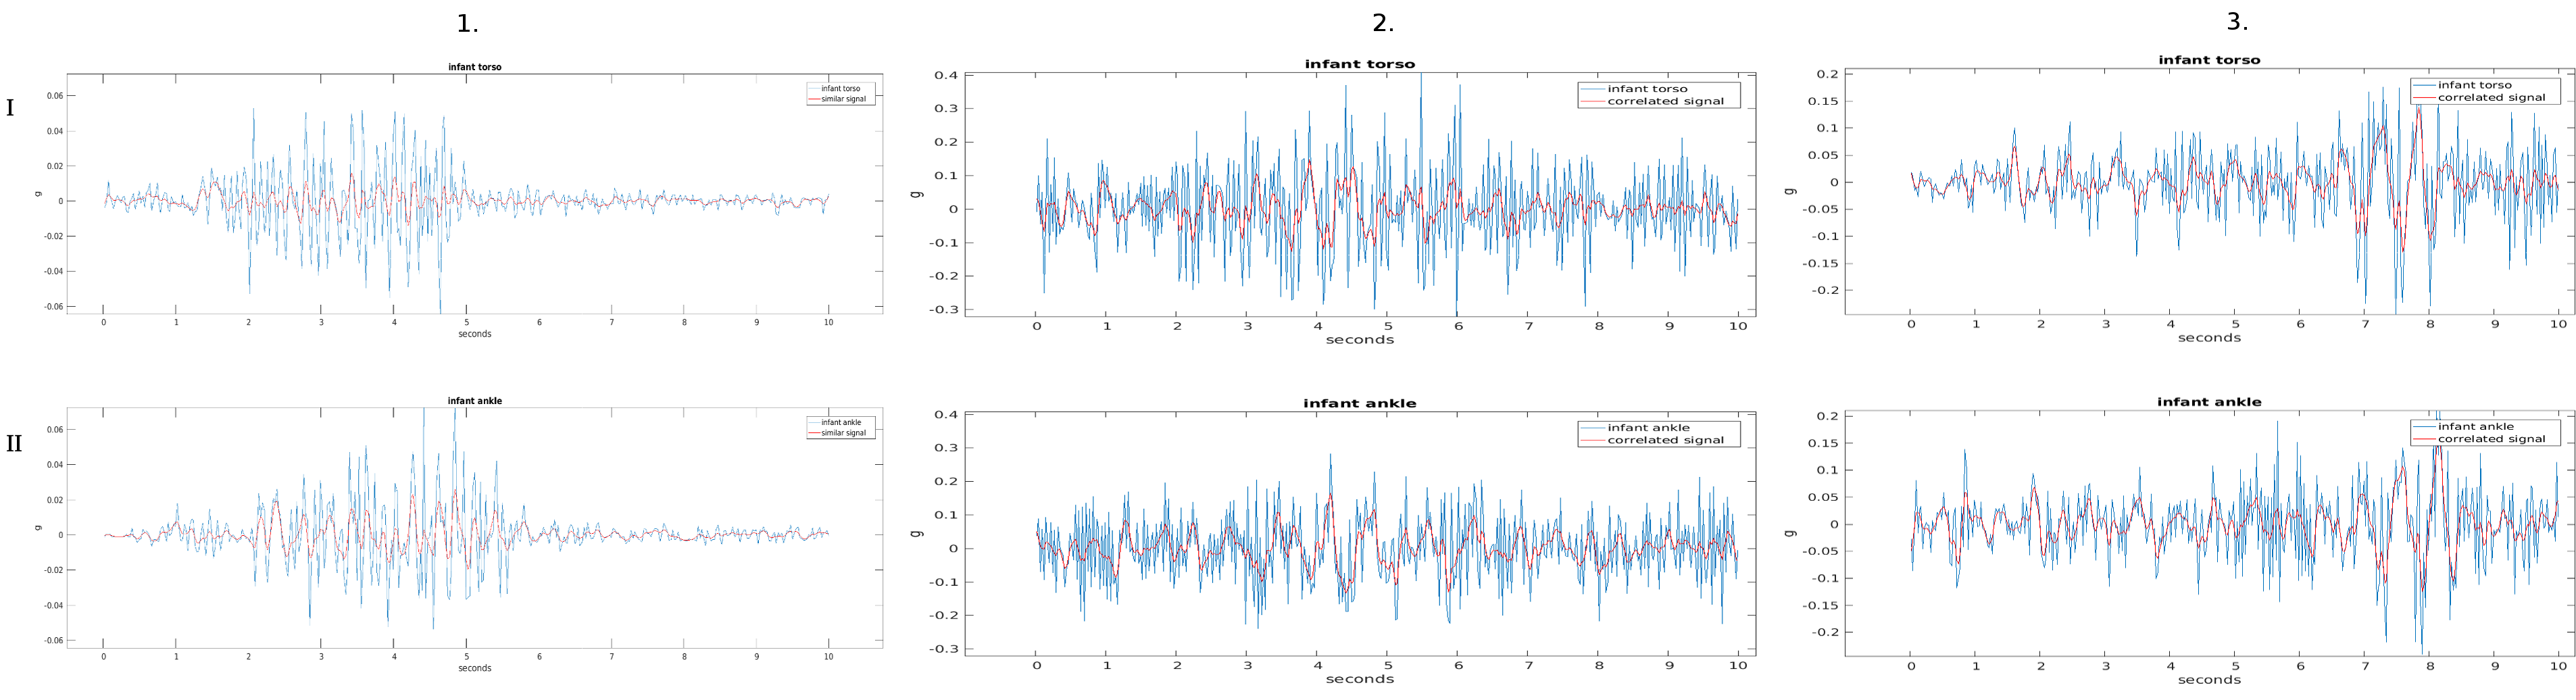
\includegraphics[width=15cm, height=6cm]{differences.png}
\caption{First plot showing a slight time lag, second plot showing larger intensities on the torso placed monitor and the third plot showing the presence of other accelerations and noise.}
\end{figure}\\
One of the basic issues with such an approach is that without a well defined training data set, we can not be certain that the underlying similarity between the measurements is due to contributing accelerations from the caretaker. The vibrations from infants kicking movement could be picked up by the torso placed monitor and might exhibit similarity with the ankle placed monitor although the least will have a substantial amount of additional accelerations. Second, we can not be sure whether in windows, where the two measurements would appear to be uncorrelated, there is an absence of contributing accelerations from the caretaker or these were just recorded so significantly different. A methodological issue is also presented by the estimation of significance and validity of the derived Pearsons correlation coefficient. Statistical inference tests, for Pearson's correlation coefficient commonly used in population studies, require a few assumptions to be met. Principally they are sensitive to the data distribution and require the data to be normally distributed, otherwise the results could be misleading. With each window of a windowed measurement, we are only interested in that particular window and no general hypothesis is attempted to be proven about the data from which the sample was taken from, but rather just the descriptive statistics are being compared. For that reason, a simple permutation test should be a better estimation rather than using the Fisher transformation, which is most used in practice and in computer languages as well as statistics tools. For such reason, the necessary prior testing for the assumption of normality can be left out, as it is unlikely that it will be met by the accelerometer data distribution, which is skewed and distorted most of the time. While one would commonly use a Spear mans rank-order correlation in cases where the data is not normally distributed, this is not appropriate in the case of comparing the similarity of two time-series as comparing the orders of ranked time points would not make sense. Nevertheless, simple Pearsons correlation coefficient and the corresponding level of significance derived with the permutation test will not always be as accurate as desired, especially in the presence of substantial additional accelerations and time lags in each of the two variables. Better methods around these issues had been developed and purposed[11][12][13], but the level of complexity exceeds the one set for this project. 
\\As large differences, additional accelerations and time lags can still influence the correlation coefficient, one has to consider the degree of measurement summarization, before calculating the correlation coefficient. Even though Figure 8 and 9 exhibit similar patterns in the original summaries of the torso and ankle placed measurement, the overall proportion of windows, where the correlation coefficient is large enough and significant, turns out to be very small. To get the desired results in approach \textbf{D}, the summarized measure of absolute intensities has to be used, as in approaches \textbf{B} and \textbf{C}.\\ 
Absolute intensities were calculated for windows of 200 points, which corresponds to 5 seconds. Correlation coefficient is obtained with the build-in function \textit{corr}, for windows of 24 absolute intensities, which corresponds to 2 minutes, sliding with a step size 12, which corresponds to 1 minute. P-value is obtained using the permutation test with 10 repetitions. If p-value is insignificant, correlation coefficient is set to 0. While sliding, the first half will overlap with the previous window. Therefor, previous correlation coefficient is compared with the current and the biggest is used for correction of the first half of the current window, while the second half is corrected with the current correlation coefficient. The final result is the ankle placed measurement, where windowed accelerations were decreased by the correlation coefficient of absolute intensities. Average SD of the apparent \textit{infant being moved} blocks is decreased by an average of 57.9\% and the average absolute intensity by an average of 58.5\%. Figure 12 shows how the result is different from the approach \textit{B} and figure 13 shows how the result is different from the approach \textit{C}.
\begin{figure}[h]
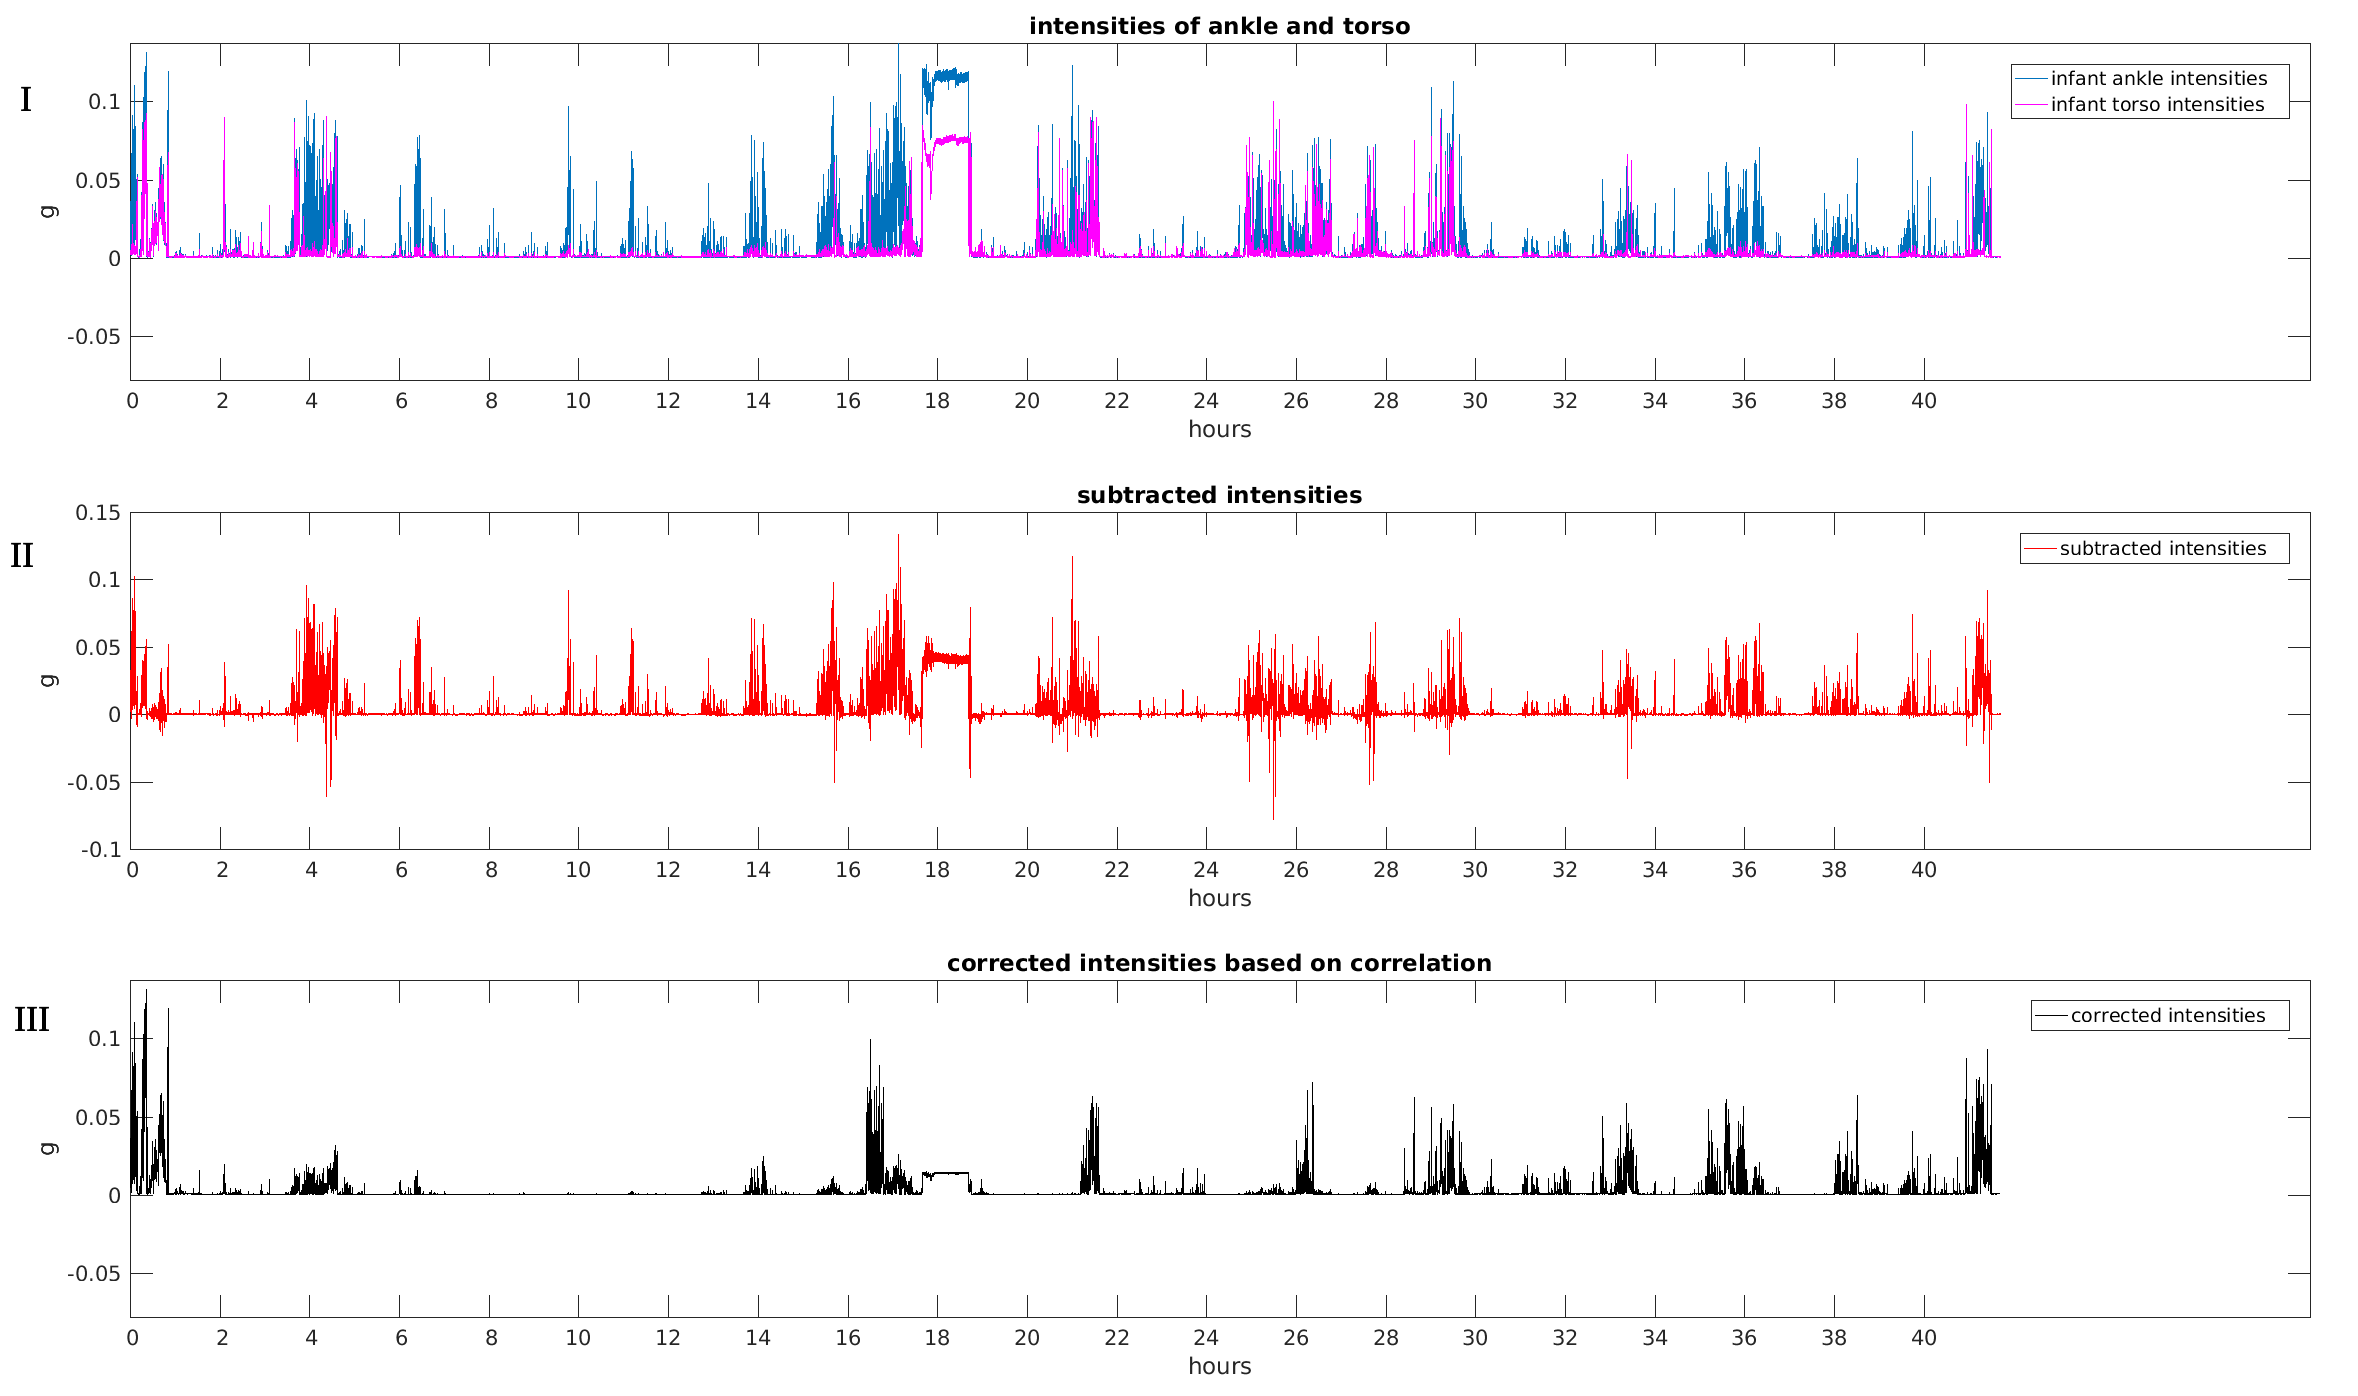
\includegraphics[width=15cm, height=6.5cm]{CorrectedIntensitiesCorrelation.png}
\caption{Example of the different results from approach \textbf{B} and \textbf{D} regarding the absolute intensities, which are no longer negative in approach \textbf{D}.}
\end{figure}

\begin{figure}[h]
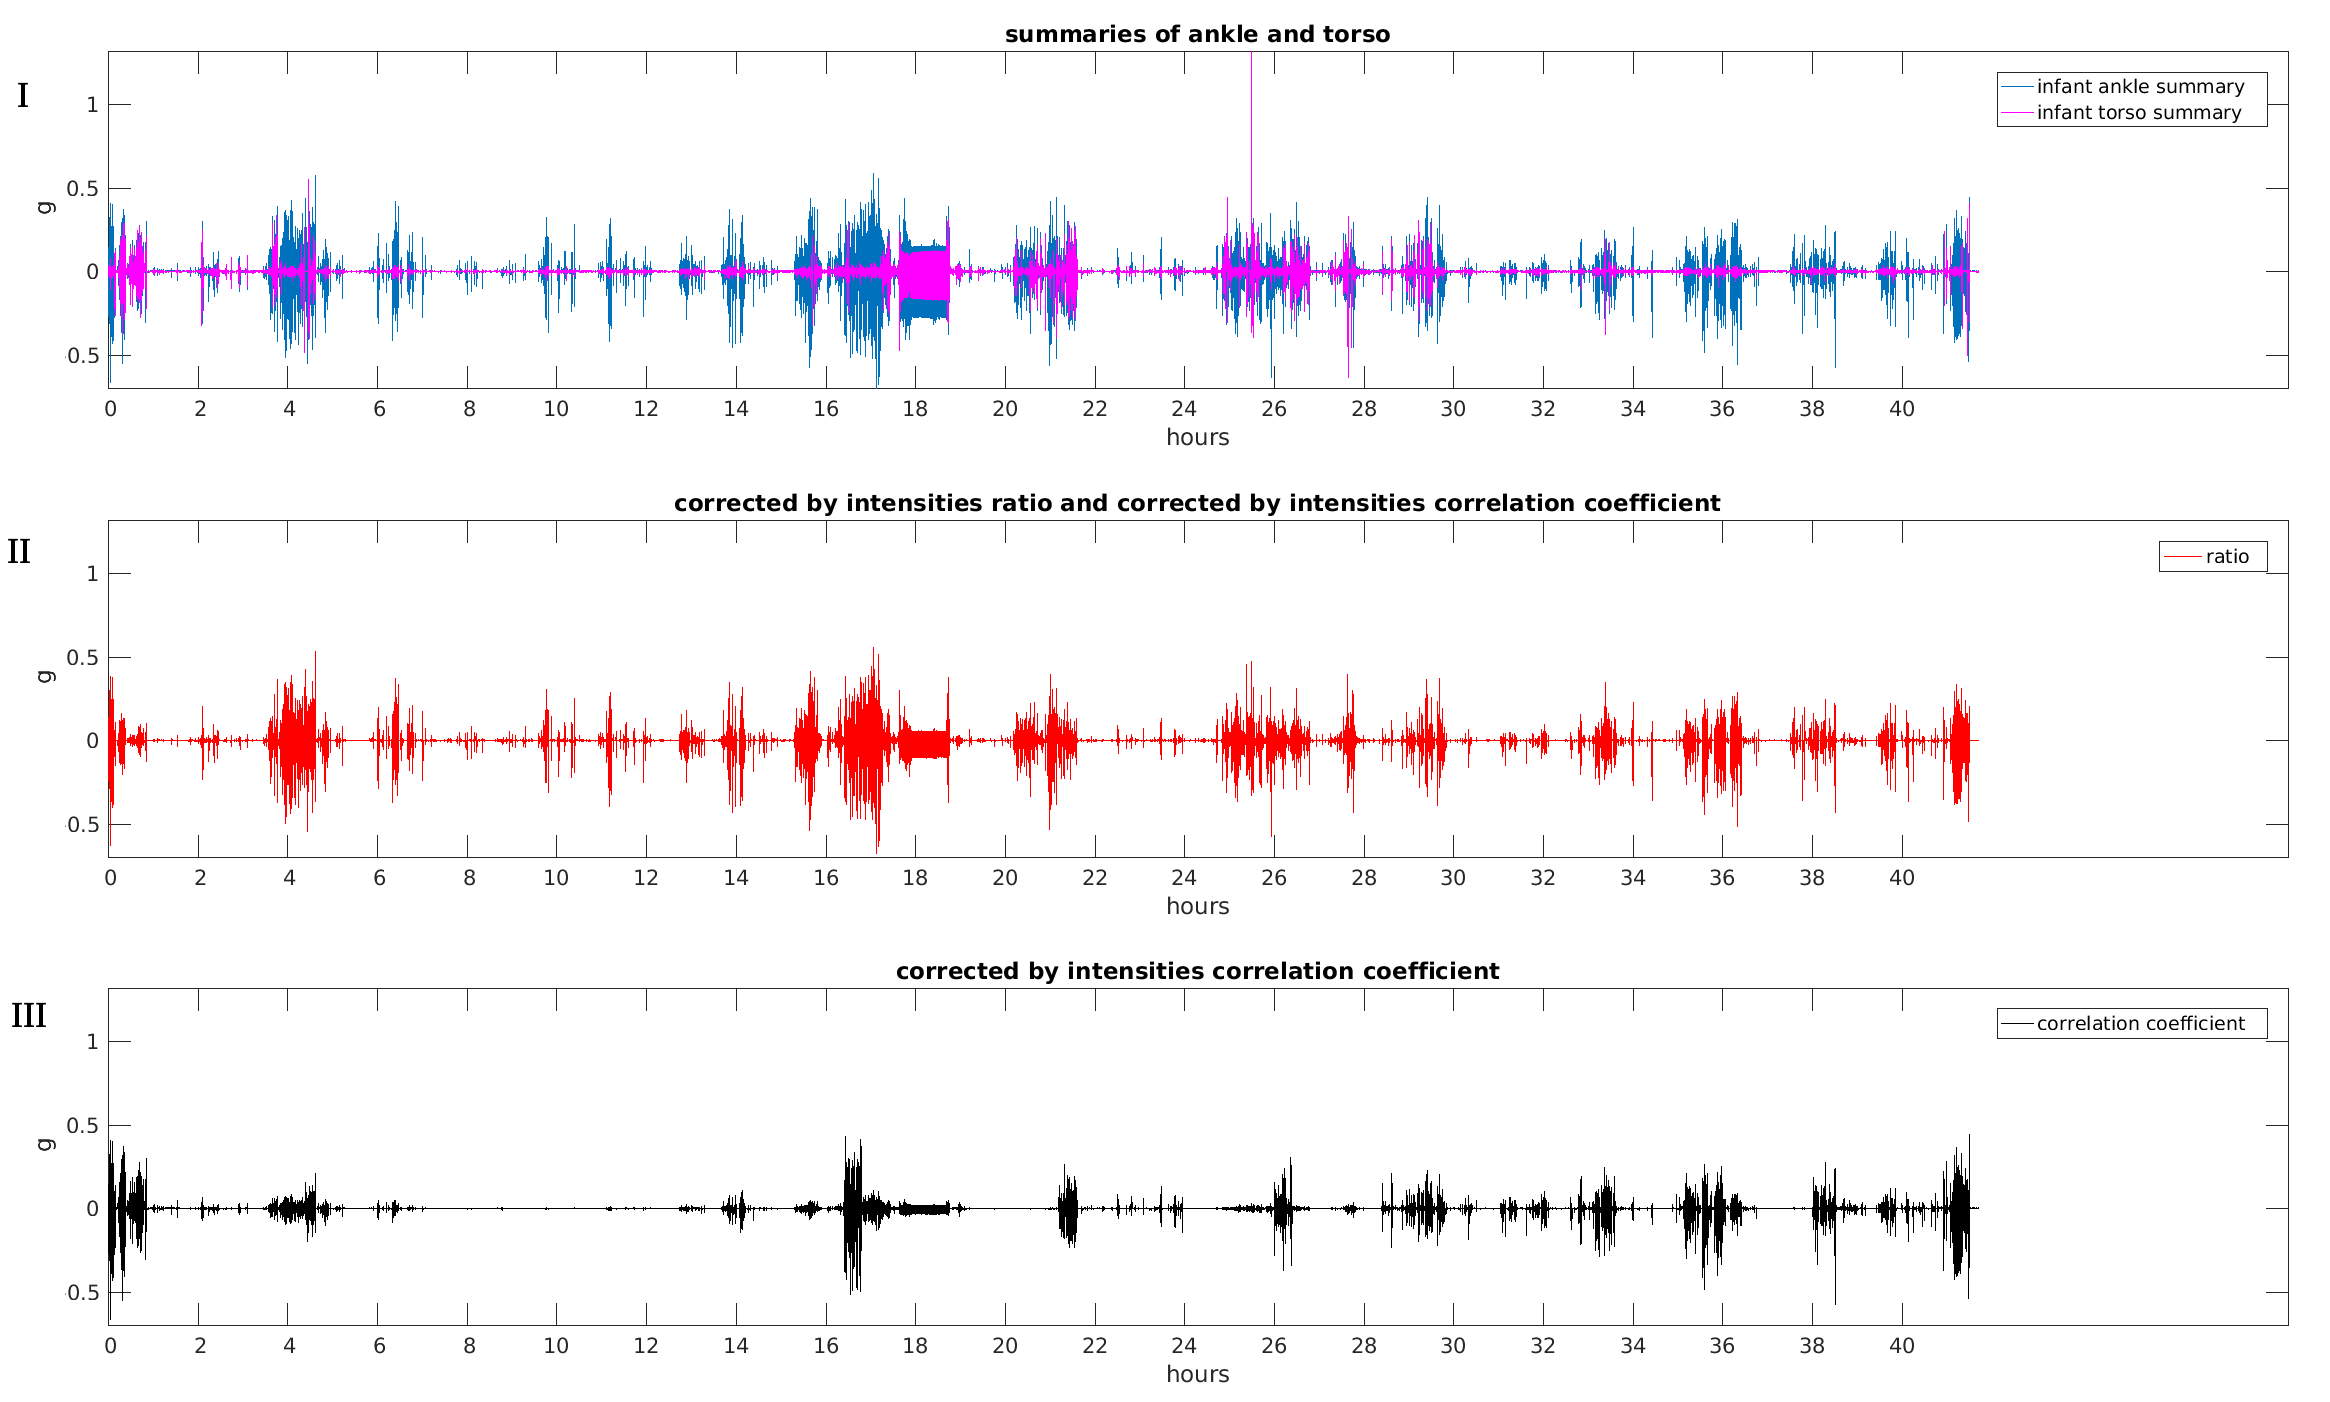
\includegraphics[width=15cm, height=7cm]{CorrectedIntensitiesCorrelation_result.png}
\caption{Example of the different results from approach \textbf{C} and \textbf{D}. One can see substantially less left-overs from the contributing accelerations in the approach \textbf{D}.}
\end{figure}
\\
In approach \textbf{D} even more parameters had to be set, whose values have a great effect on the final outcome. Without a training data set, these parameters were again set by trial and examination and their optimum is uncertain.
Along with the basic issues present, approach \textbf{D} is still not certain enough and one would like to extract PA without having to consider whether the correction for the contributing accelerations was accurate enough. This leads to the final approach \textbf{E}, where all the blocks detected as \textit{infant being moved} are simply removed from the measurement and are therefore excluded from the future extraction of PA. Example of these blocks in Figure 5.
\\Each approach results in an ankle placed measurement, where the contributed accelerations were attempted to be removed. Those results are used for PA extraction, where further comparison and assessment of the different approaches can be made.
}

%------------------------------------------------

\section{Physical activity}
\fontsize{11.25pt}{11.1pt}\selectfont {
Mothers characteristics in pregnancy, along with the infants characteristics post-partum, can provide significant information when studying fetal programming[14][15][16]. Infants at 4 months post-partum will not yet have been substantially exposed to and influenced by the environment outside the intrauterine environment, especially when it comes to PA, which is still completely instinct at that point and can there for be considered \textit{pre-programmed}.
By being able to accurately estimate infants PA, many research questions could be addressed. 
\\Although accelerometers are commonly used to estimate subjects PA, there are several issues that can lead to incorrect or uncertain results that disable further analysis. When estimating infants PA with accelerometers, the major issue is represented by the contributing accelerations of the infants caretaker. In this project, several approaches to correct for these contributions were implemented and analyzed. Different outcomes of different approaches are used to extract PA and the results are compared and further analyzed.
\subsection{Extraction}
PA was extracted from the corrected or remaining measurements, after removal of data points of non-wear time, summarization, correction for the gravitational component and the correction for \textit{infant being moved}. In approaches where the result of the \textit{infant being moved} correction is in the form of the original summary, PA is extracted based on the increased SD in a windowed measurement. Window size was set to 10 seconds, which corresponds to 400 data points and the step size was set to 1 seconds, which corresponds to 40 data points. SD threshold was set to 0.005 g. The results from the approach \textbf{A} are not used for PA extraction, as they are  obviously not suitable. In the approach \textbf{B}, the result is in a form of subtracted absolute intensities, which can be negative due to inadequacy of the approach. Extracting PA from the intensities can be done by setting a threshold for the intensity size, defining all intensities over that threshold as due to PA. When extracting PA based on the results from approach \textbf{B}, one can observe the results are not going to be accurate, example Figure 14. There are obvious left-overs from the contributing accelerations, which are now detected as infants PA, while the negative intensities disrupt the PA blocks.
\begin{figure}[h]
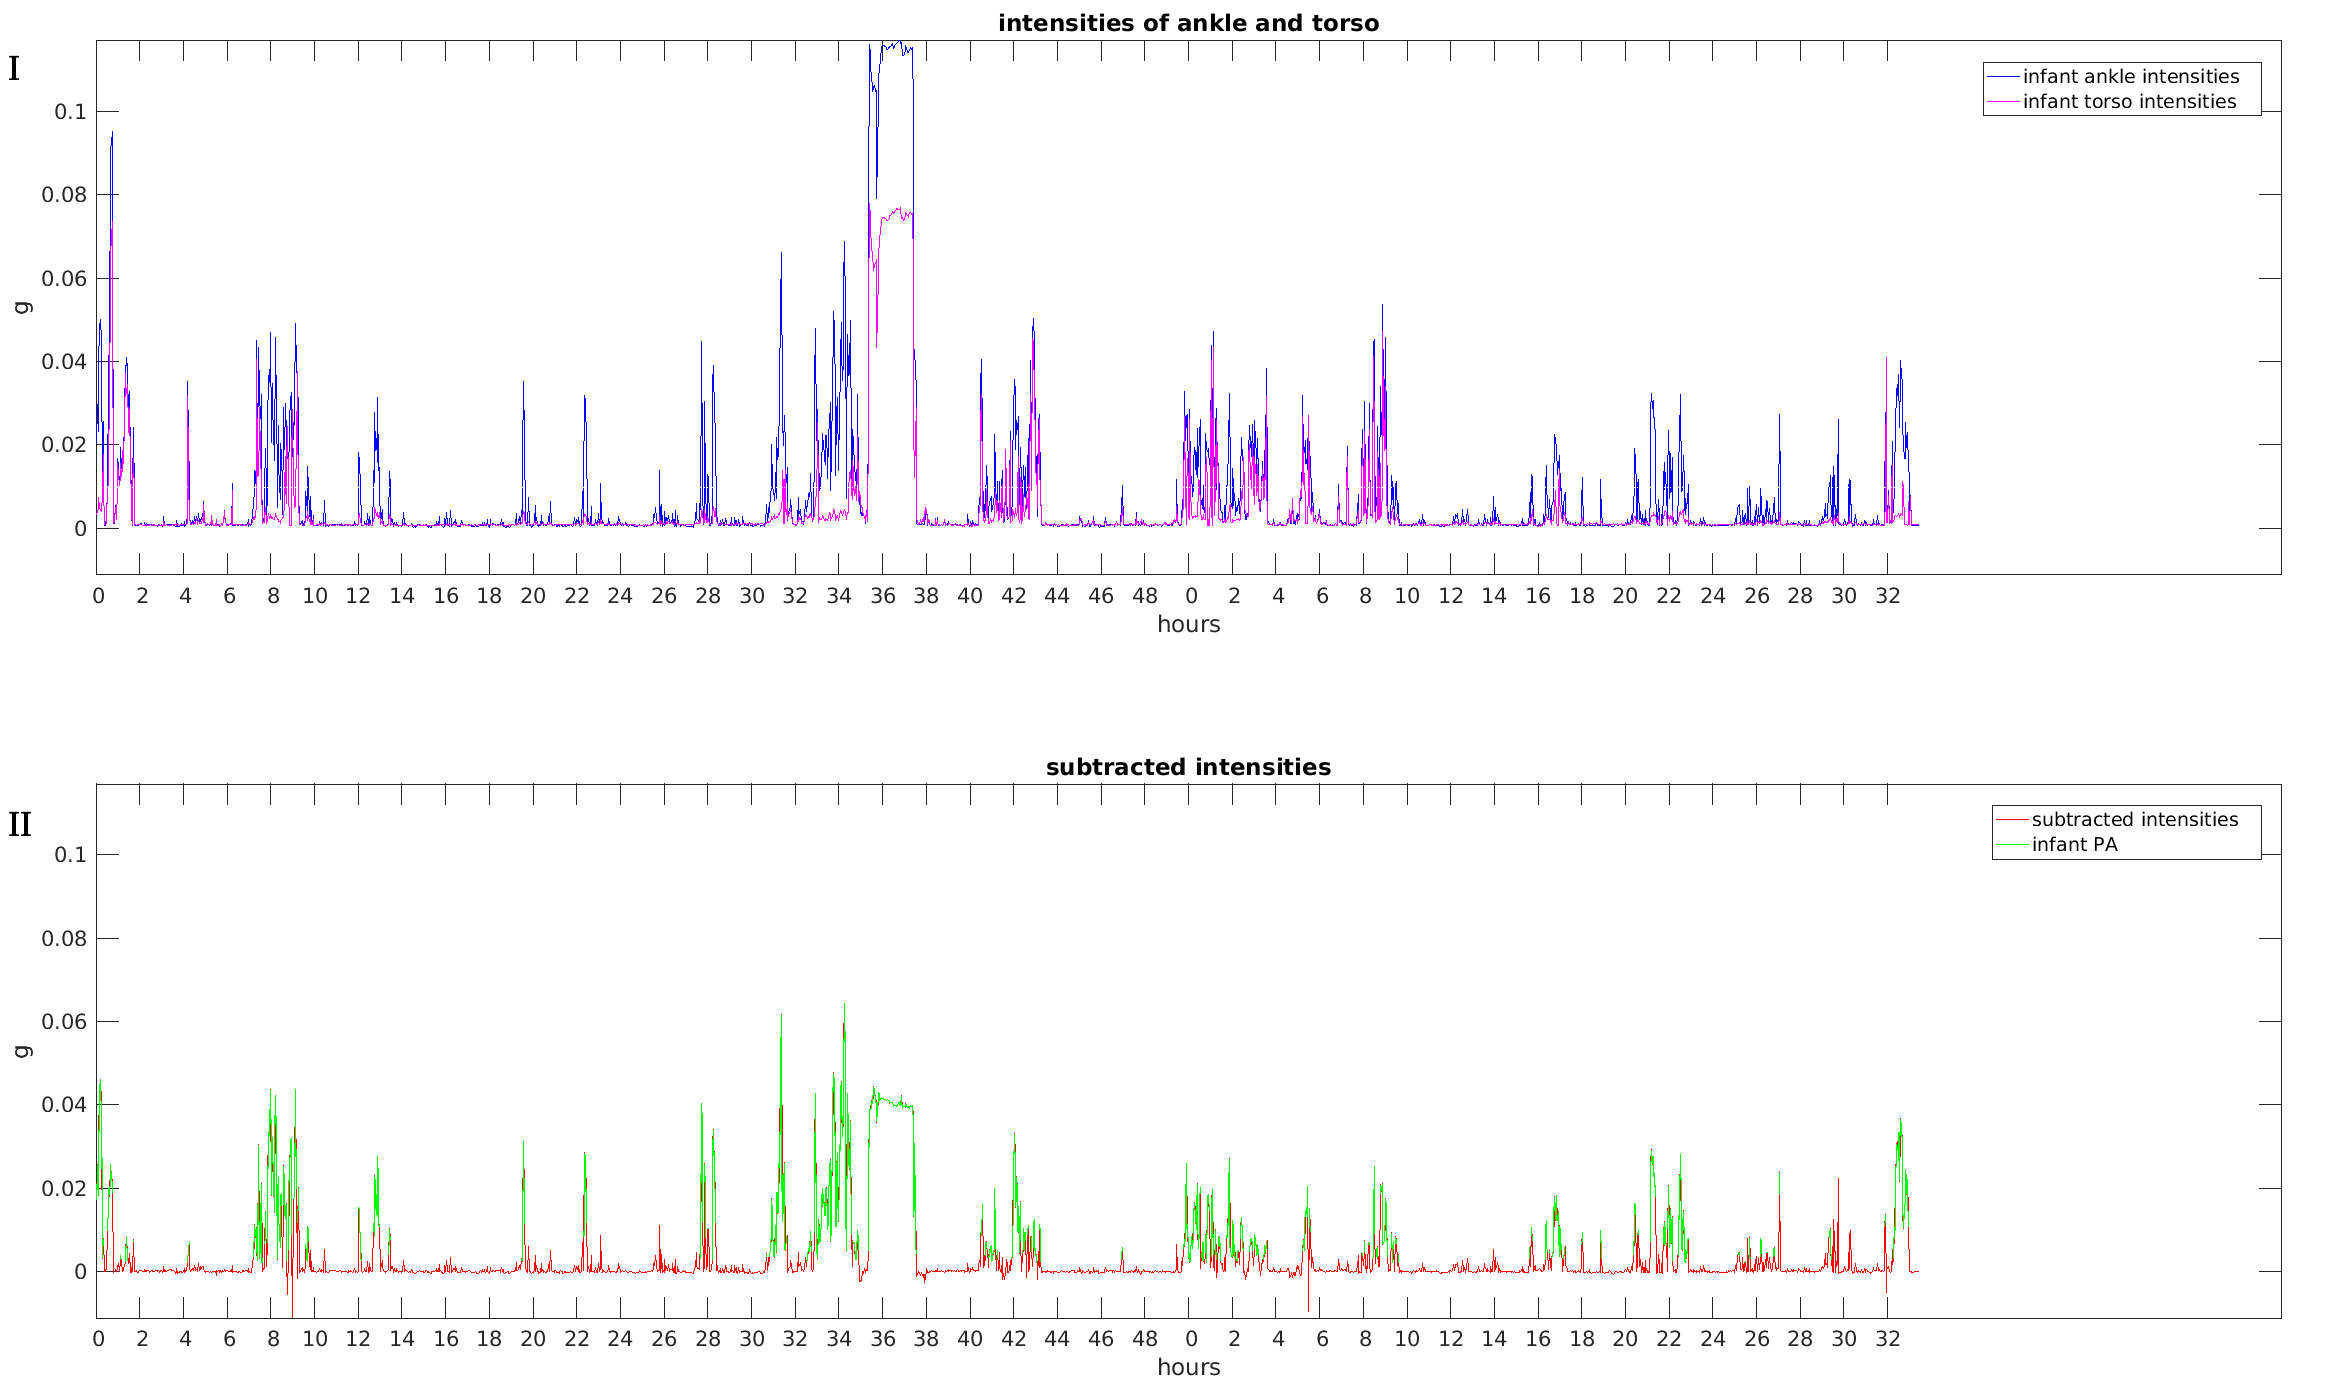
\includegraphics[width=15cm, height=7cm]{SubtractedIntensitiesPA.png}
\caption{PA extraction after approach \textbf{B} exhibits the consequences of the negative features of the approach.}
\end{figure}
\\
Since approach \textbf{C} is based on the same principle as \textbf{B}, they will possess the same degree of inaccuracy on a certain level. The difference is, that in approach \textbf{C}, PA extraction can be done with more precision as the measurement is not summarized into intensities and even though, subtractions causing negative intensities, have the same inaccurate effect, PA extraction might not be so influenced by it, as it might not contribute so substantially to the SD of a certain window. Results of PA extraction based on the approach \textbf{C} in Figure 15.
\begin{figure}[h]
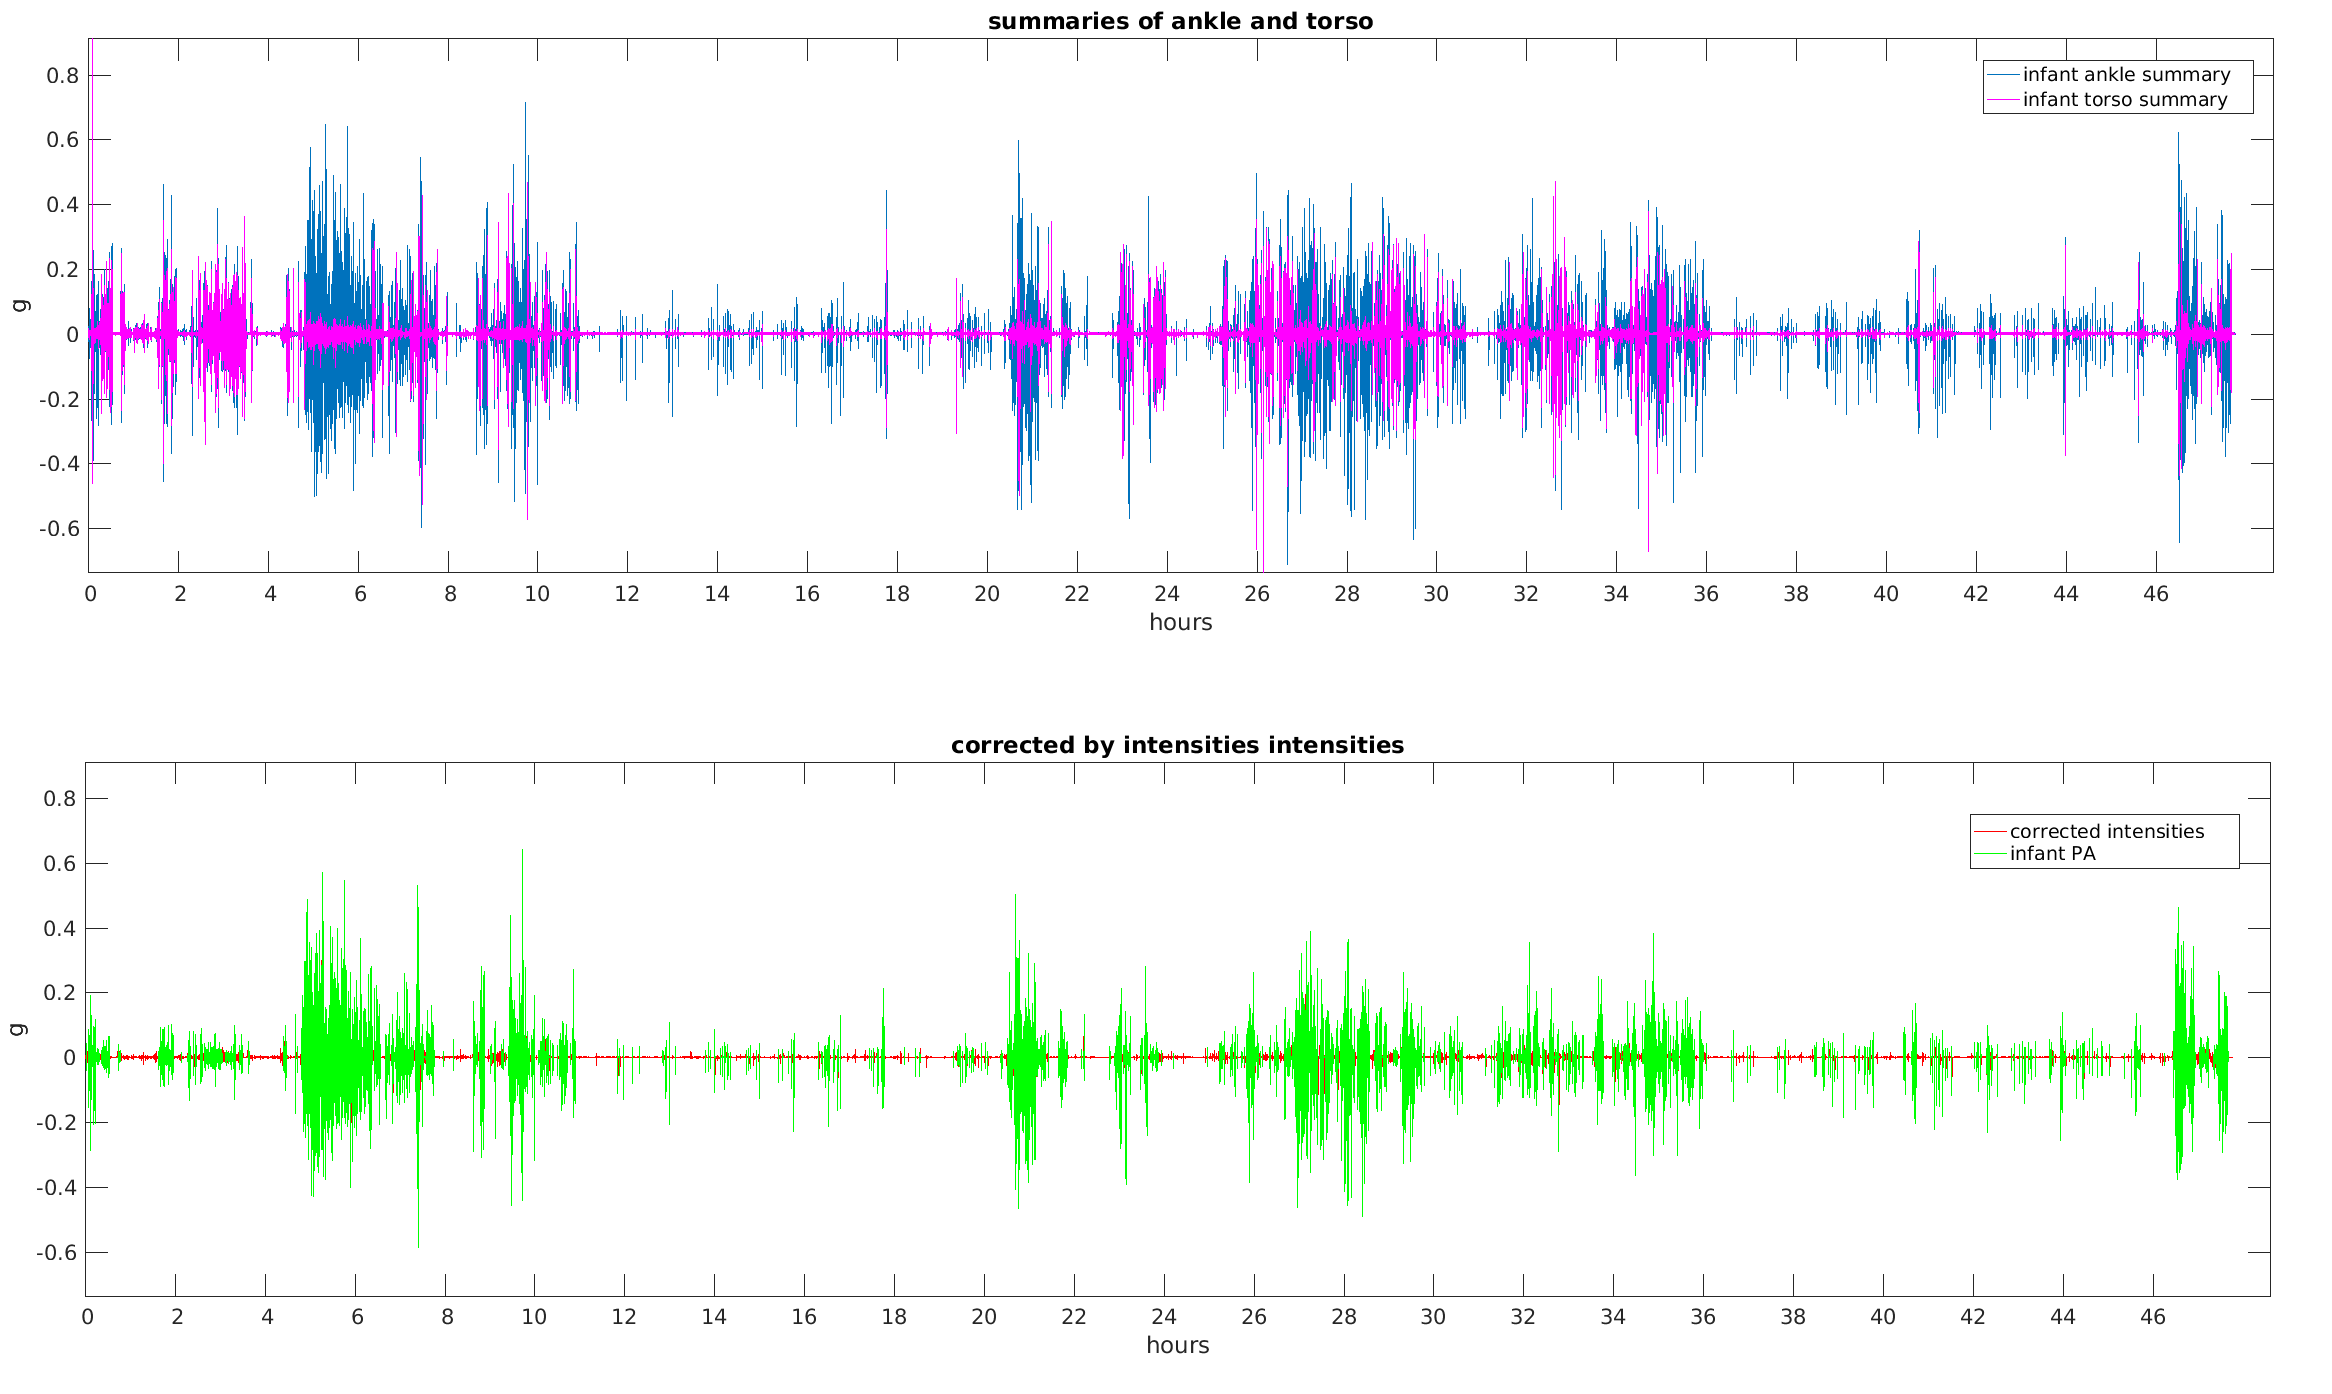
\includegraphics[width=15cm, height=7cm]{CorrectedIntensitiesPA.png}
\caption{PA extraction after approach \textbf{C}.}
\end{figure}
\\
Based on approach \textbf{D}, PA can be extracted from the measurement in a form of absolute intensities or in a form of the original summary. Example of PA extraction from absolute intensities based on approach \textbf{D} in Figure 16 and example of PA extraction from the original summary in Figure 17. 

\begin{figure}[h]
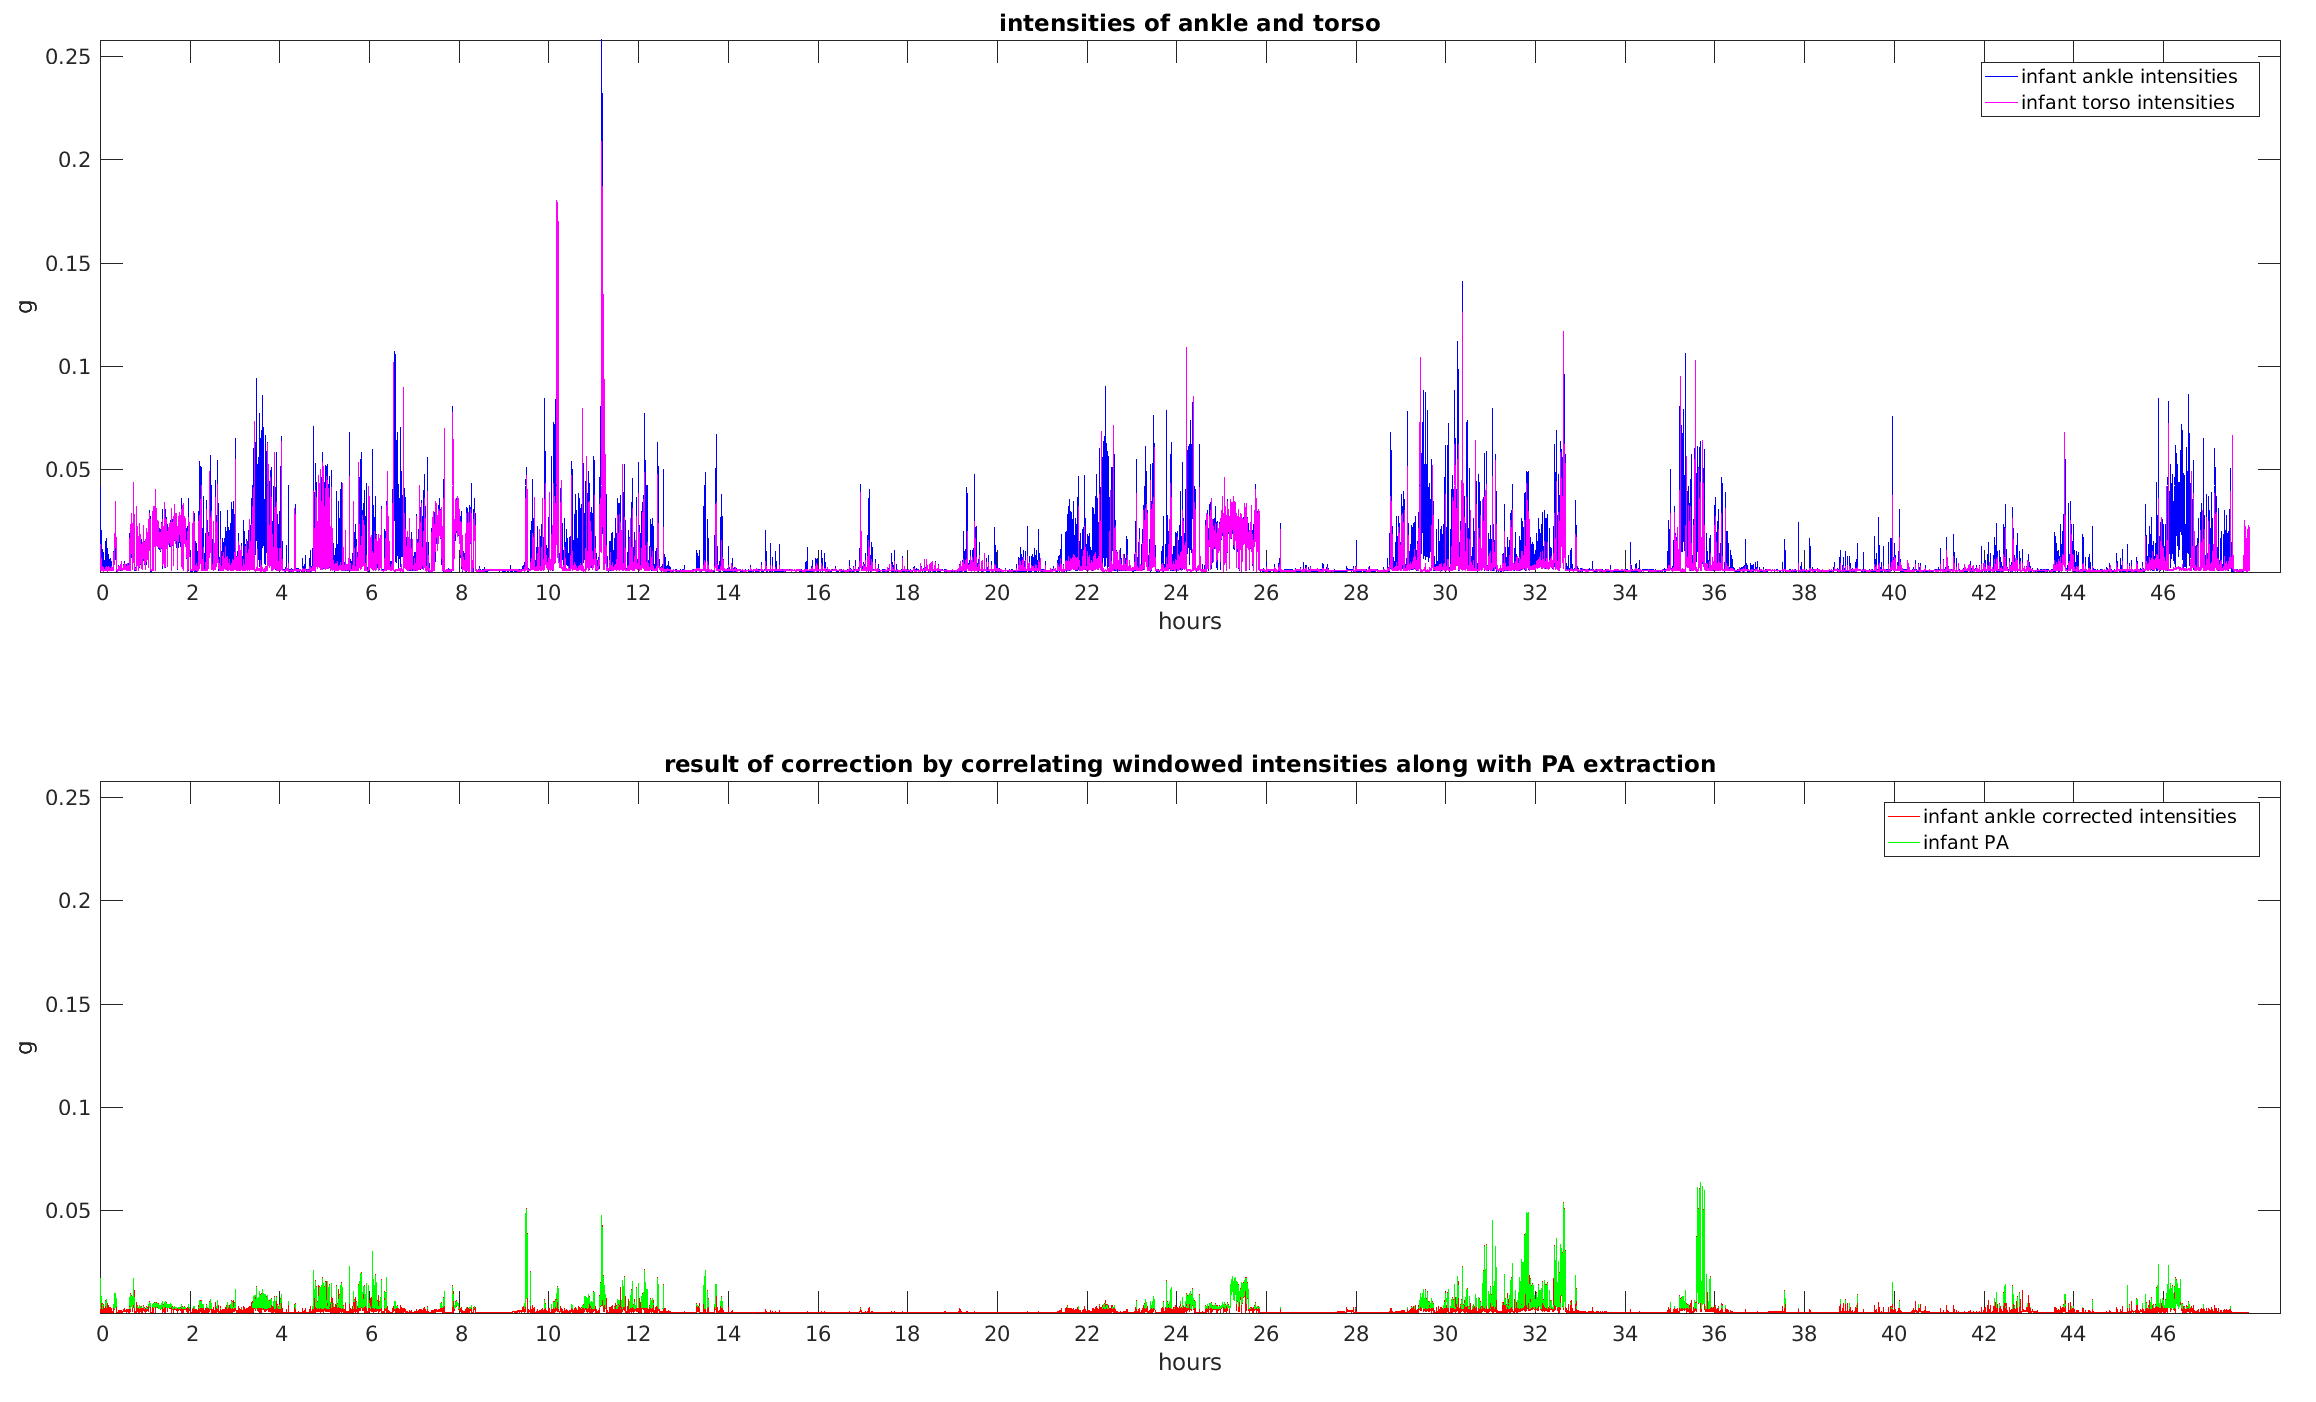
\includegraphics[width=15cm, height=7cm]{CorrectedIntensitiesCorrelationResultPA.png}
\caption{PA extraction from absolute intensities, based on approach \textbf{D}.}
\end{figure}

\begin{figure}[h]
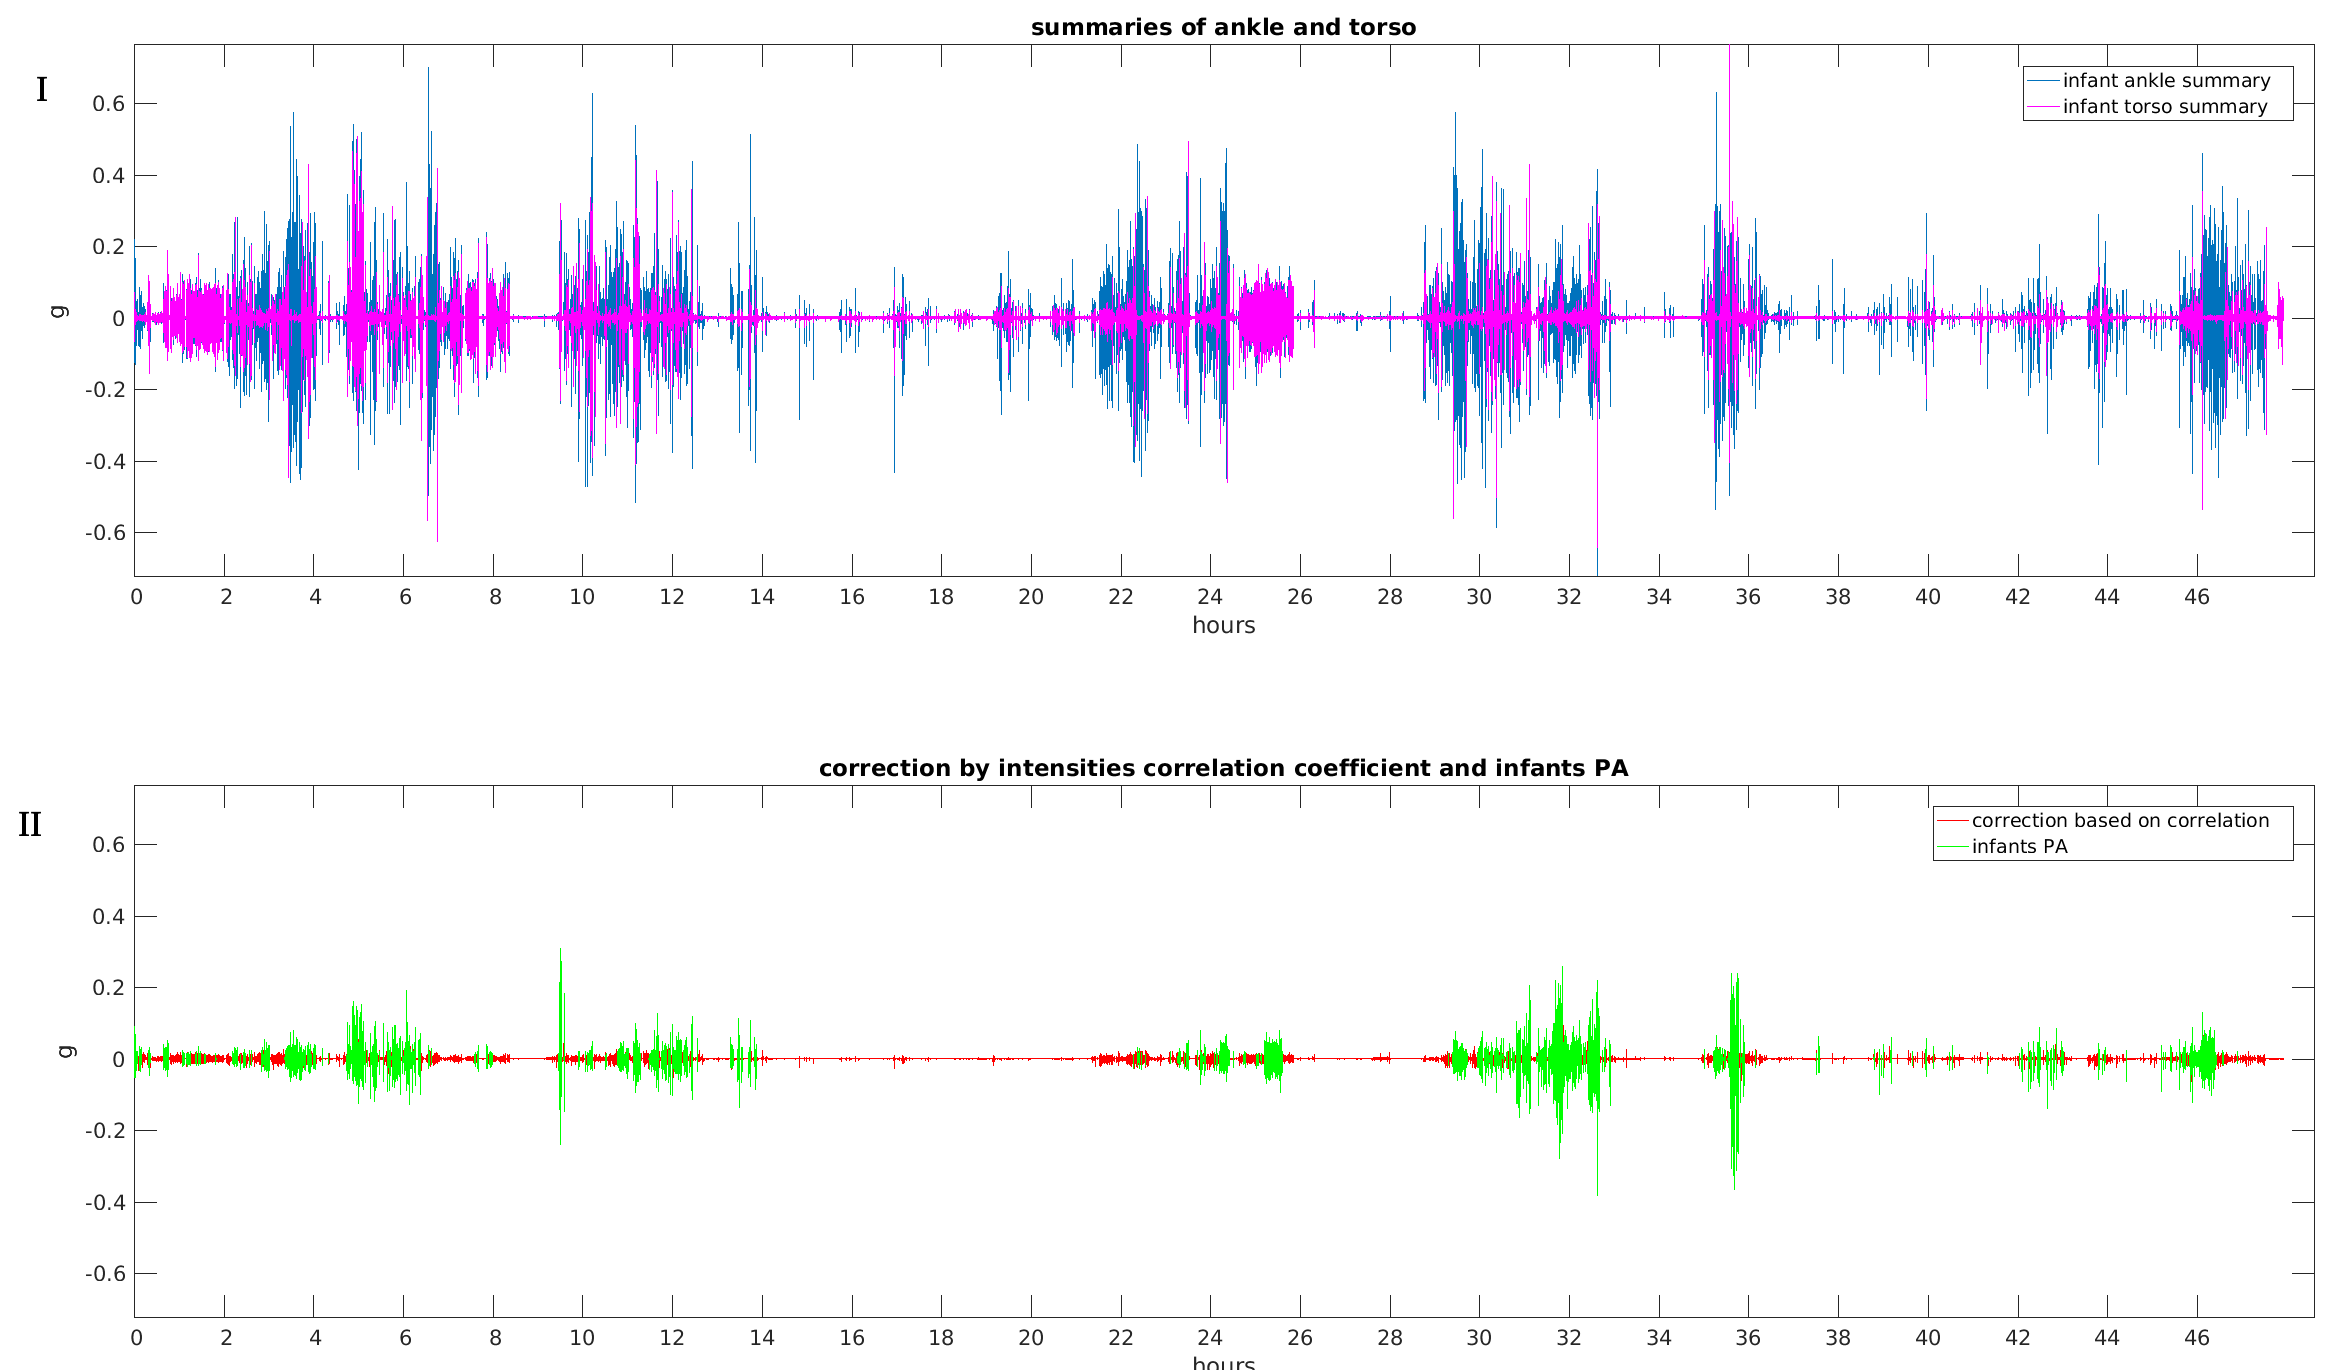
\includegraphics[width=15cm, height=7cm]{CorrectedCorrelationResultPA.png}
\caption{PA extraction from the original summary, based on approach \textbf{D}.}
\end{figure}

In both cases, one can observe less left overs of the contributing accelerations and in the first case PA is extracted more accurately than in approach \textbf{B} since there are no more negative subtracted intensities left. Nevertheless, PA can be extracted with more precision when the measurement is in the form of the original summary, so when considering approach \textbf{D}, only that result will be further analyzed.
Last approach is approach \textbf{E}, where all the apparent blocks of \textit{infant being moved} are simply removed from the measurement and only the rest is used to extract PA. Example of the result in Figure 18, where the \textit{infant being moved} blocks are marked red and the infant PA green.
\begin{figure}[h]
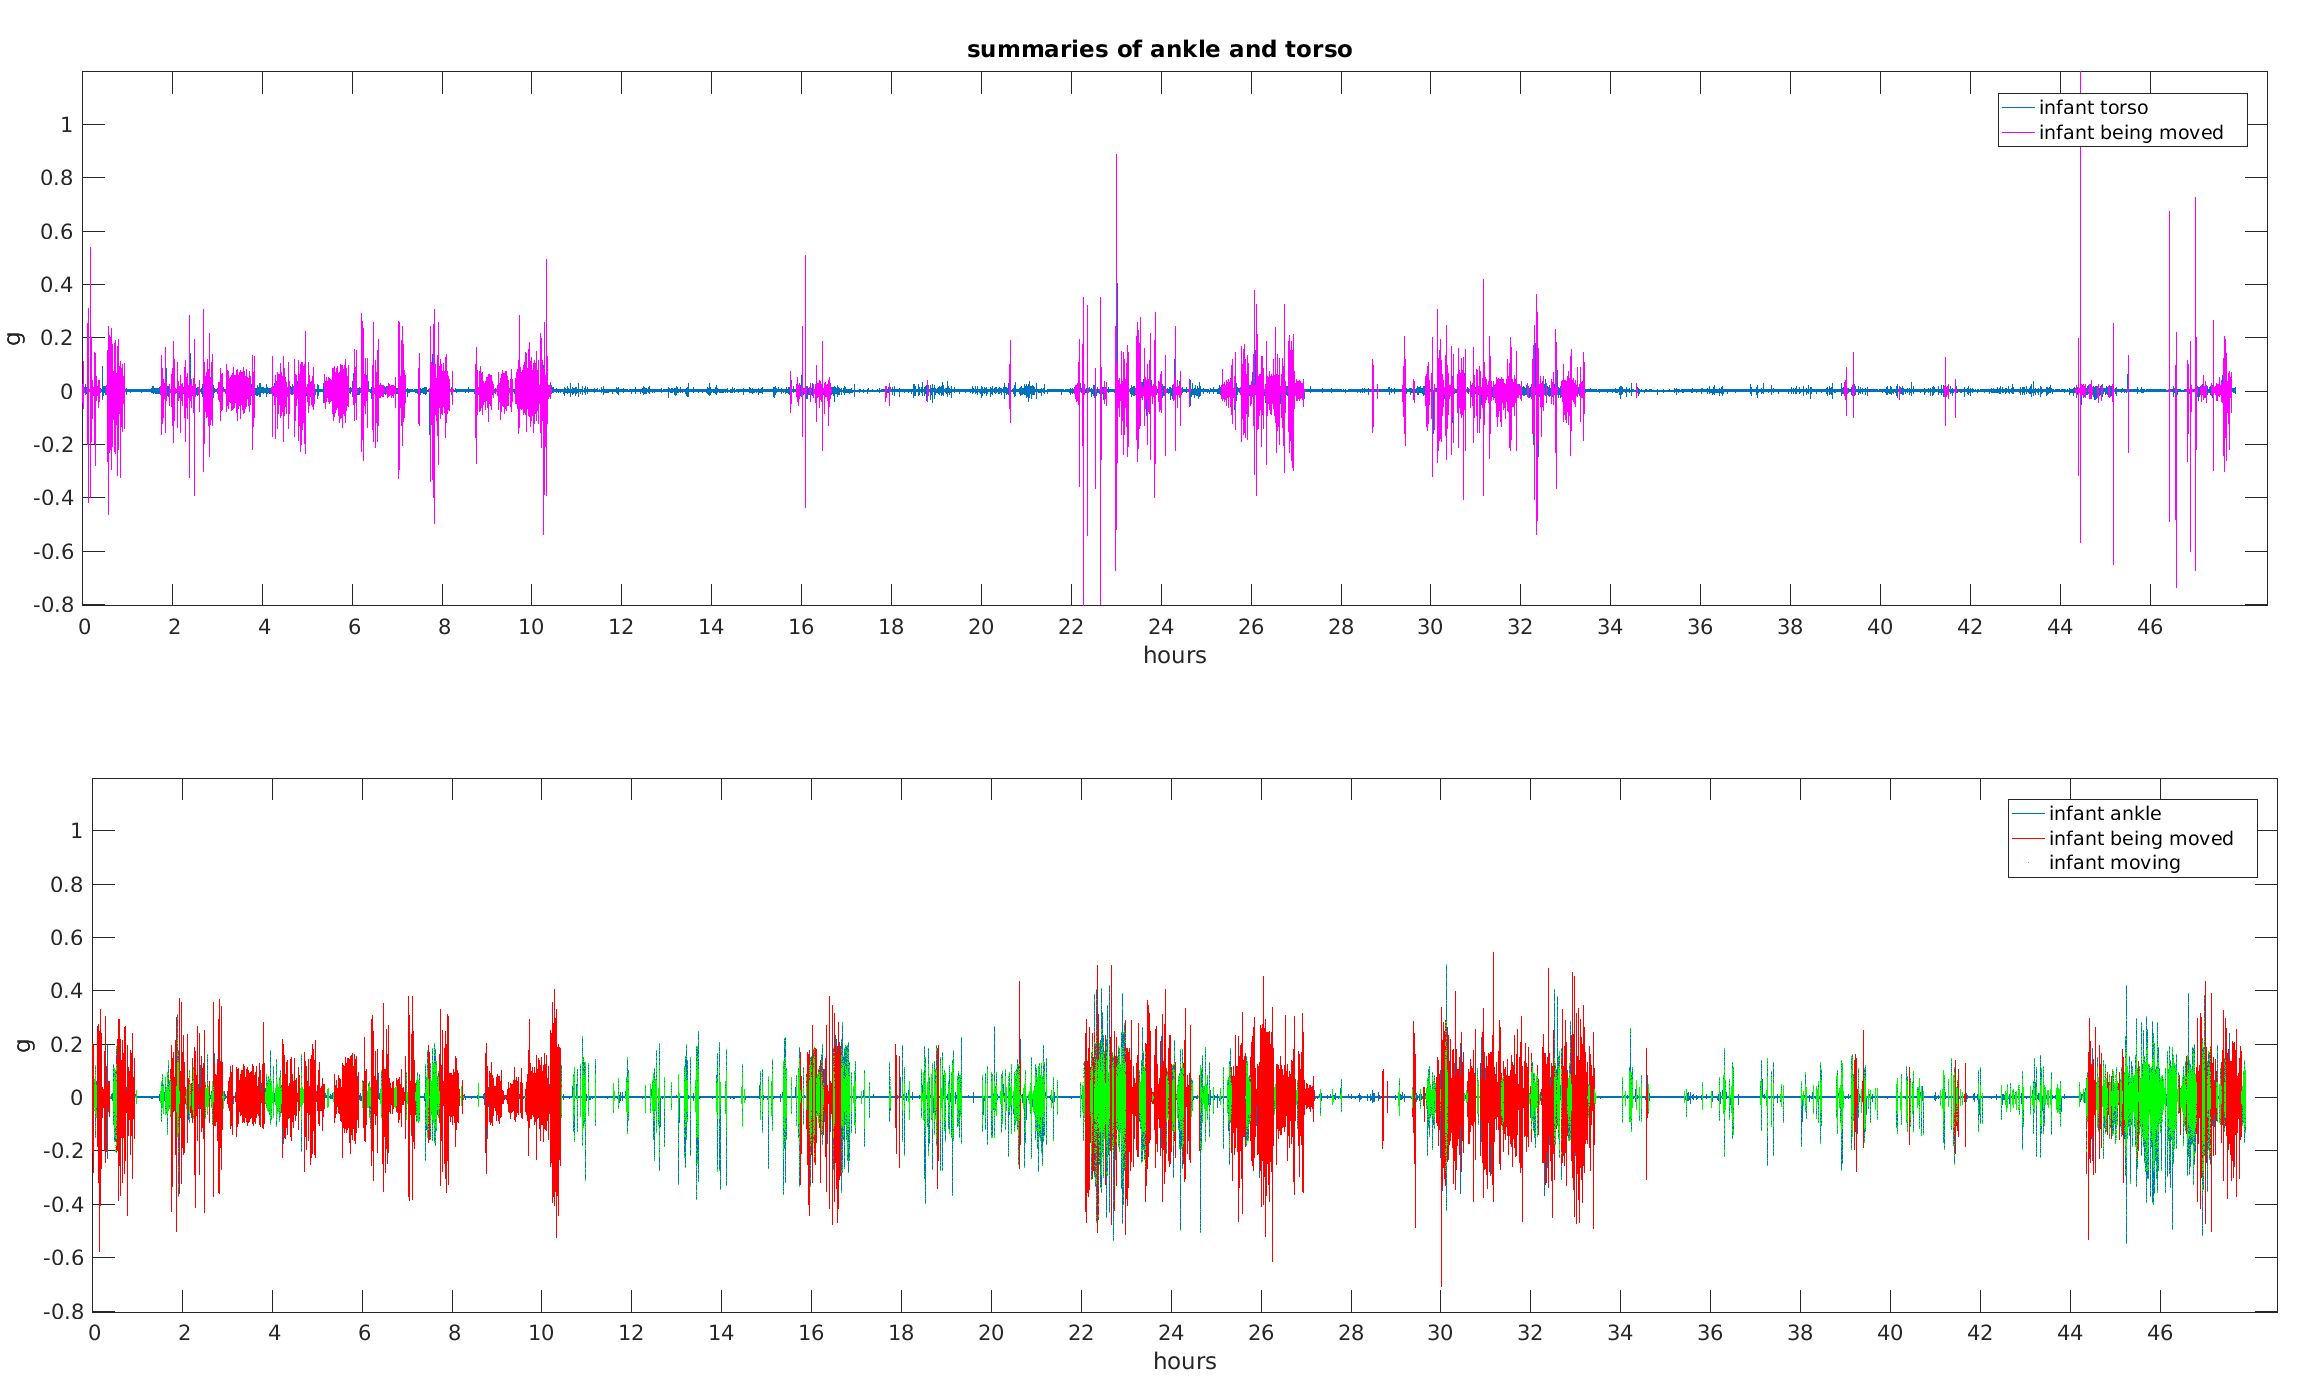
\includegraphics[width=15cm, height=6.5cm]{approachEPA.png}
\caption{PA extraction from the remaining original summary, where all the \textit{infant being moved} blocks had been removed.}
\end{figure}

\subsection{Analysis}
Overall, the proportion of time the infant was in PA differed between the various approaches. One could already expect that extracting and analyzing PA based on the approach A will be meaningless, as the majority of accelerations present are still due to infant being moved. In fact, when comparing the proportion of time infant is supposed to spent in PA based on approach A, to the proportion of time the infant was being moved, over all subjects, Spearmans rank correlation coefficients results in 0.84 with p-value 0, example in Figure 19.
\begin{figure}[h]
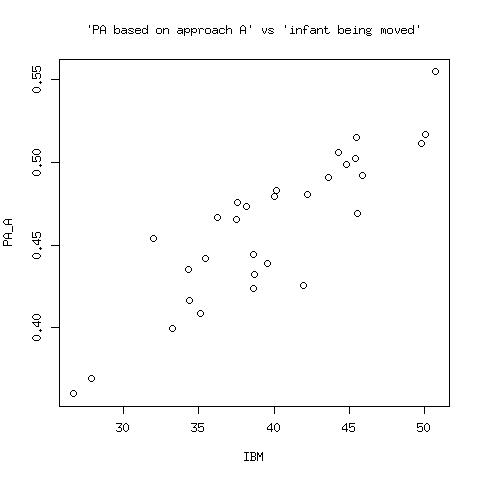
\includegraphics[width=9cm, height=9cm]{PAAIBM.jpg}
\caption{Comparing the proportion of time in PA after approach \textbf{A} and proportion of time infant was being moved, over all subjects.}
\end{figure}
\\
This makes sense, as PA and \textit{infant being moved} blocks are extracted with the same procedure, using a slightly different SD cutpoint. Considering this, along with the observation, that subtraction does not remove contributing accelerations, but in fact enhances them, it is not surprising these proportions end up being very similar. With approaches \textbf{B} and \textbf{C} better results can be expected. PA extraction based on approach \textbf{B} resulted in infant being in PA on an average of 34.3\% of his 'own time', with min 23.0\%, max 45.0\% and SD 5.4\%, while based on approach \textbf{C}, infant was in PA on an average 32.5\% of his 'own time', with min 21.9\%, max 42.0\% and SD 4.8\%. \\These numbers are similar, although one would expect them to differ more, since first approach extracts PA from subtracted absolute intensities that can be negative. One explanation could be that these errors even out and by averaging over the subjects, the final outcome will be similar, example of a boxplot of the two extracted PA values over all subjects in Figure 20.
\begin{figure}[h]
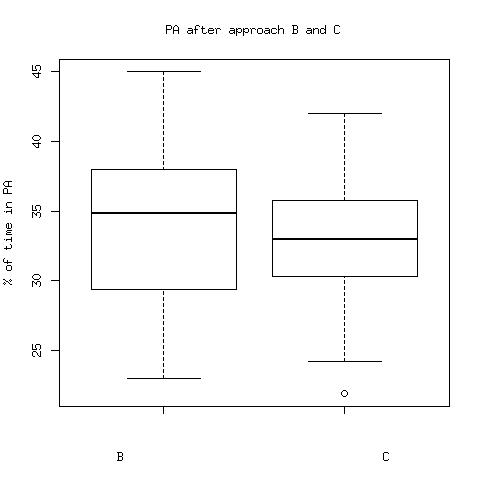
\includegraphics[width=7cm, height=7cm]{boxplotPABC.jpg}
\caption{Comparing the proportion of time in PA between approaches \textbf{B} and \textbf{C}, over all subjects.}
\end{figure}
\\
 When examining these numbers along with the proportion of time the infant was being moved, plots still exhibit slight correlation between the two variables, with exception of a few outliers, example in Figure 21. 
\begin{figure}[h]
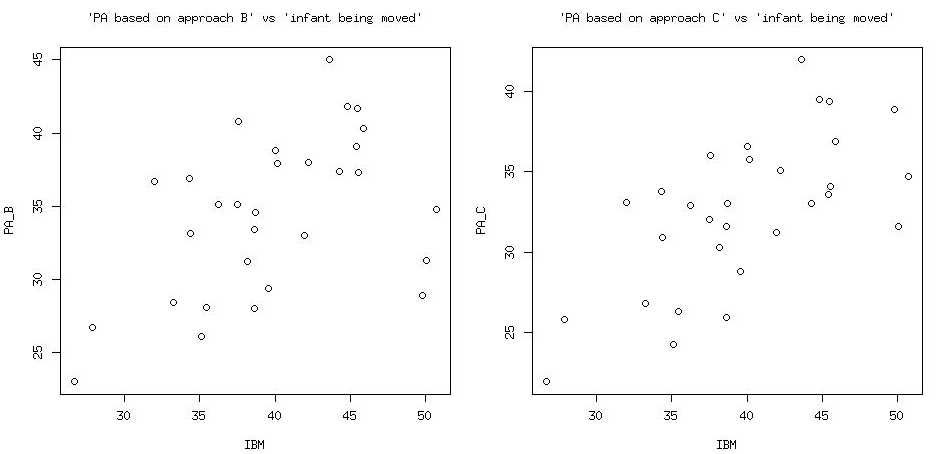
\includegraphics[width=14cm, height=7cm]{corrPABPACIBM.png}
\caption{Comparing the relationship between the proportions of infants PA and being moved time.}
\end{figure}
\\
Over all subjects, the proportion of time in PA after approach \textbf{B} and the proportion of time the infant was being moved produced a Spearmans rank correlation coefficient of 0.48 with p-value 0.0072, while with the proportion of time in PA after approach \textbf{C} the coefficient was 0.64 with p-value \textit{2e-04}. One could speculate that such correlation is due to the left overs of the contributing accelerations, although there is a chance that caretakers influence infants own PA by interaction.
Moving on to approach \textbf{D}, PA extraction resulted in an average of 25.5\% of infants 'own time', with min 12.3\%, max 47.6\% and SD 0.09\%. Spearmans rank correlation coefficient for the comparison of the proportion of time in PA after approach \textbf{D} and the proportion of time the infant was being moved resulted in 0.41 with a p-value 0.0236. Scatterplot of proportion of time in PA vs. proportion of time being moved in Figure 22.\\
\begin{figure}[h]
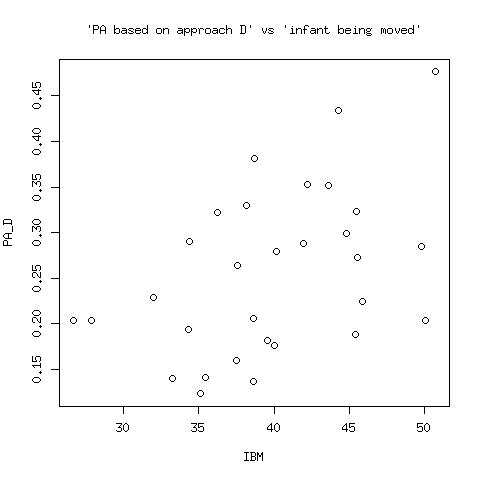
\includegraphics[width=7cm, height=7cm]{scatterplotPADIBM.jpg}
\caption{Comparing the proportion of time in PA after approach \textbf{D} and the proportion of time the infant was being moved, over all subjects.}
\end{figure}

Although there is less significant correlation then in previous approaches, there is still a substantial amount, but again with uncertainty, whether this due to the contributing accelerations, same procedure of extraction, or caretakers interference. So far, all the extracted PA variables were liable to be confounded by the contributing accelerations. With the last approach, one would expect to have no correlation with the proportion of the time infant was moved, since it had all been removed and the final PA variable should not be confounded. \\
While the resulting proportion of time the infant was in PA, based on approach \textbf{E}, was on average 19.4\% with minimum 12.8\%, maximum 26.0\% and SD 3.2\%, when correlating the proportion of time in PA with the proportion of time being moved, Spearmans rank correlation coefficient results in -0.42 with p-value 0.0218. The sign and quantity of correlation imply that there is a negative relationship between the two. Scatterplot of the proportion of time in PA vs. proportion of time being moved in Figure 23. Considering only the methodological reasons for this implication, one could speculate that by removing all the parts where the infant was being moved, in a short time period of 48 hours, will result in very little measurement left for the infants PA to be detected. Keeping in mind the infants at 4 month old age are very dependent on the caretaker, especially while awake, one can also speculate, the majority of measurement left after approach \textbf{E} will belong to the time when infant was sleeping. Such interference could leave consequences, even if the final PA variable is normalized with the amount of time left after the approach. More can be explored and validated with the help of diaries, kept by the infants mothers. This is discussed in the next chapter, where the rest of the extracted variables are also analyzed. 
 \begin{figure}[h!]
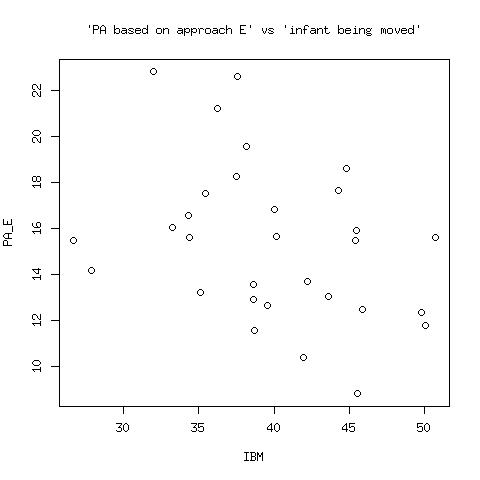
\includegraphics[width=6.7cm, height=6.7cm]{scatterplotPAEIBM.jpg}
\caption{Relationship between the proportion of infants PA after approach \textbf{E} and proportion of being moved time.}
\end{figure}
\\
}
\section{Validation against sleeping and feeding diary}
\fontsize{11.25pt}{11.1pt}\selectfont {
During the free living experiment, the mothers were instructed to keep a diary of the infants feeding and sleeping habits, along with other valuable information regarding the experiment, like for example removal and reattachment of the accelerometer. All subjects had the diary data available, except one, where the diary was missing. The diary consisted of printed forms, example in Supplements. Besides a few exceptions, the mothers started keeping diary notations on the second day, from midnight on. This already presents a drawback, since the accelerometer data was recorded only for 48 hours from the morning of the first day on, meaning that out of those 48 hours, approximately 15 hours will not have corresponding diary notations. \\Since the diaries were filled by handwriting, the notations inside had to be digitized, to enable automatic comparison and validation. Although one could attempt to achieve this automatically by document scanning and image analysis, such approach would be too complicated and time-consuming for the needs of this project, where only 30 documents had to processed. Therefor these documents were examined manually, which was nevertheless still very time consuming and error prone. For several reasons, a substantial amount of error was also introduced by the mothers keeping the notations. Mainly this was due to rounding up the noted time, having trouble keeping up with notations and then not being able to recall the time of certain occurrences.\\
First, the diary forms enabled notation of accelerometer removal and reattachment, where the mothers had to note which of the accelerometers is being taken off, corresponding comments and the absolute time of removal and reattachment. Frequently, the mothers commented that the accelerometer was forgotten to be put back on after removal and the times noted are therefor approximate. Secondly, the diary forms included a schedule over 24 hours, over a week, where the mothers were instructed to note the infants sleeping time with a stroke. As one can see in the Supplements, the sleeping schedule is not so big, meaning that the space for one hour is very small. Consequently, it was difficult for the mothers to keep accurate and consistent notations of infants sleeping time. The noted times became even less accurate, when the mothers forgot to note regularly and had to therefor recall the approximate times of sleeping. For the validation and comparison of data analysis, absolute timestamps were needed and had to be therefor created manually, by examining these schedules, which introduced even more error. The final timestamps were therefor liable to be very approximate and error prone and one should begin to question whether comparison and validation against such timestamps is useful and valid itself. Last, mothers were instructed to keep a diary of infants feeding time, by noting down the begin time and duration of feeding, along with a few other comments, not relevant for this project. Feeding notations had to be transformed into begin and end timestamps, to enable validation and comparison. Example of the final data table, created manually based on a diary in Table 1.

\begin{table}[h]\tiny
\begin{tabular}{|l|l|l|l|l|l|}
\hline
feeding start       & feeding finish      & sleeping start      & sleeping finish     & torso monitor detached & torso monitor reattached \\ \hline
2009-02-10 08:20:00 & 2009-02-10 08:50:00 & 2009-02-10 00:00:00 & 2009-02-10 08:10:00 & 2009-02-09 11:30:00    & 2009-02-09 16:00:00 \\ \hline
2009-02-10 09:30:00 & 2009-02-10 10:00:00 & 2009-02-10 13:00:00 & 2009-02-10 13:40:00 & 2009-02-09 18:30:00    & 2009-02-09 20:00:00 \\ \hline
2009-02-10 10:00:00 & 2009-02-10 11:00:00 & 2009-02-10 15:00:00 & 2009-02-10 15:25:00 & 2009-02-10 21:10:00    & 2009-02-11 08:15:00 \\ \hline
2009-02-10 14:15:00 & 2009-02-10 15:00:00 & 2009-02-10 19:00:00 & 2009-02-10 19:40:00 &                        &                     \\ \hline
2009-02-10 15:50:00 & 2009-02-10 16:20:00 & 2009-02-10 22:20:00 & 2009-02-11 08:25:00 &                        &                     \\ \hline
2009-02-10 17:30:00 & 2009-02-10 17:45:00 & 2009-02-11 10:30:00 & 2009-02-11 11:40:00 &                        &                     \\ \hline
2009-02-10 20:00:00 & 2009-02-10 20:30:00 & 2009-02-11 13:25:00 & 2009-02-11 14:00:00 &                        &                     \\ \hline
2009-02-10 21:00:00 & 2009-02-10 21:15:00 & 2009-02-11 19:30:00 & 2009-02-11 20:05:00 &                        &                     \\ \hline
2009-02-11 08:20:00 & 2009-02-11 09:30:00 & 2009-02-11 22:00:00 & 2009-02-12 08:25:00 &                        &                     \\ \hline
2009-02-11 11:30:00 & 2009-02-11 11:45:00 &                     &                     &                        &                     \\ \hline
2009-02-11 14:15:00 & 2009-02-11 15:00:00 &                     &                     &                        &                     \\ \hline
2009-02-11 15:00:00 & 2009-02-11 16:00:00 &                     &                     &                        &                     \\ \hline
2009-02-11 16:50:00 & 2009-02-11 17:15:00 &                     &                     &                        &                     \\ \hline
2009-02-11 17:30:00 & 2009-02-11 17:45:00 &                     &                     &                        &                     \\ \hline
2009-02-11 19:15:00 & 2009-02-11 19:35:00 &                     &                     &                        &                     \\ \hline
2009-02-11 20:30:00 & 2009-02-11 21:00:00 &                     &                     &                        &                     \\ \hline
2009-02-11 21:15:00 & 2009-02-11 21:30:00 &                     &                     &                        &                     \\ \hline
\end{tabular}
\caption{Example of a data table, created manually based on a diary kept by the infants mother.}
\end{table}
Overall, the handwritten diaries were hard to examine, due to unclear handwriting and sloppy notes which often did not make sense. It became likely that the diaries will not provide the desired means for validation, especially if considering the amount of error along with the frequency of feeding and sleeping occurrences. Nevertheless, the diary timestamps were compared against the timestamps obtained through data analysis in an attempt to extract any kind of validating information. \\
First, timestamps obtained through automatic non-wear time detection were compared to the timestamps generated based on the diaries. The comparison was implemented in Python, with the help of modules \textit{pandas}, \textit{datetime} and \textit{dateutil}. Even though the exact time of the beginning and end of non-wear occurrences differed between the timestamps for an average of one hour, all the major non-wear occurrences were detected, with a few exceptions of either very short non-wear occurrences or occurrences where the accelerometer was noted as not being worn, but the measurement clearly showed movement. Based on the visual examination of plots with no-wear time marked, the timestamp differences were due to the errors in the diary based timestamps and not in the data analysis.
Second, the timestamps obtained through detection of infant being moved and the timestamps obtained through detection of infants PA were compared to the sleeping and feeding blocks noted in the diary. Ideally one would expect to have \textit{infant being moved} detected around the begin and end of sleeping blocks and all through out from begin to end of a feeding block, while there should be less \textit{infant being moved} detected, while the infant is sleeping, when there should also be substantially less infants PA. Considering the amount of error introduced with the diaries and the frequency of sleeping and feeding occurrences, it would be uninformative to compare the exact timestamps and their differences, instead, for all detected timestamps of \textit{infant being moved}, proportions of time were calculated regarding into which diary block the timestamps fell. Altogether, nine blocks were defined. A block of time where the infant was sleeping and feeding, sleeping only, feeding only, close/around of a sleeping and feeding block, close/around to sleeping only block, close/around to feeding only block, inside of a sleeping block, but also being close/around a feeding block, inside of a feeding block, but also being close/around a sleeping block and the final block being none of the above, meaning infants free awake time. Final proportions overall subject in Table 2.
\begin{table}[h]\tiny
\centering
\begin{tabular}{|p{0.5cm}|p{1cm}|p{1cm}|p{1cm}|p{1.5cm}|p{1.5cm}|p{1.5cm}|p{1.2cm}|p{1cm}|p{1cm}|p{1cm}|p{1cm}|p{1cm}|}
\hline
overall subjects & inside of a sleeping and feeding block & inside of a sleeping block only & inside of a feeding block only & close to start or end of a sleeping and feeding block & inside of a sleeping block but also close to the start or end of a feeding block & inside of a feeding block but also close to the start or end of a sleeping block & close to start or end of a sleeping block only & close to start or end of a feeding block only & not in or near feeding or sleeping block \\ \hline
mean & 0.69\%  & 38.10\%  & 3.49\%  & 2.88\%  & 2.79\%  & 0.65\%  & 16.45\%  & 5.52\%  & 29.39\% \\ \hline
min & 0\% & 26.40\%  & 0\% & 0\% & 0\% & 0\% & 8.41\% & 0.27\%  & 16.37\% \\ \hline
max & 4.77\%  & 59.02\%  & 23.87\% & 6.62\%  & 11.79\% & 3.36\%  & 27.81\%  & 16.64\%  & 45.61\% \\ \hline
SD & 1.18\% & 9.51\% & 6.98\% & 1.70\% & 2.98\%  & 0.85\%  & 5.00\% & 3.56\%  & 9.74\% \\ \hline
\end{tabular}
\caption{Table of timestamp proportions falling in certain diary blocks. }
\end{table}
\\
The biggest proportions are represented by the sleeping block only and infants free awake time, although the SD is very high with both. On average, SD is very high for all the defined blocks and the span between minimum and maximum is large, showing a substantial amount of variability between the subjects. In figures 24 and 25, examples of plots where the measurement is noted with \textit{infant being moved} blocks, sleeping and feeding blocks and night time, show the variability and the frequency of different occurrences, resulting in less informative validation. For more accurate results, the amount of day and night time should be taken into account as well, since the accelerometer data lacks 15 hours of diary data and the rest of the 33 hours will have two nights and only one day, which results in more \textit{sleeping} time.
\begin{figure}[h]
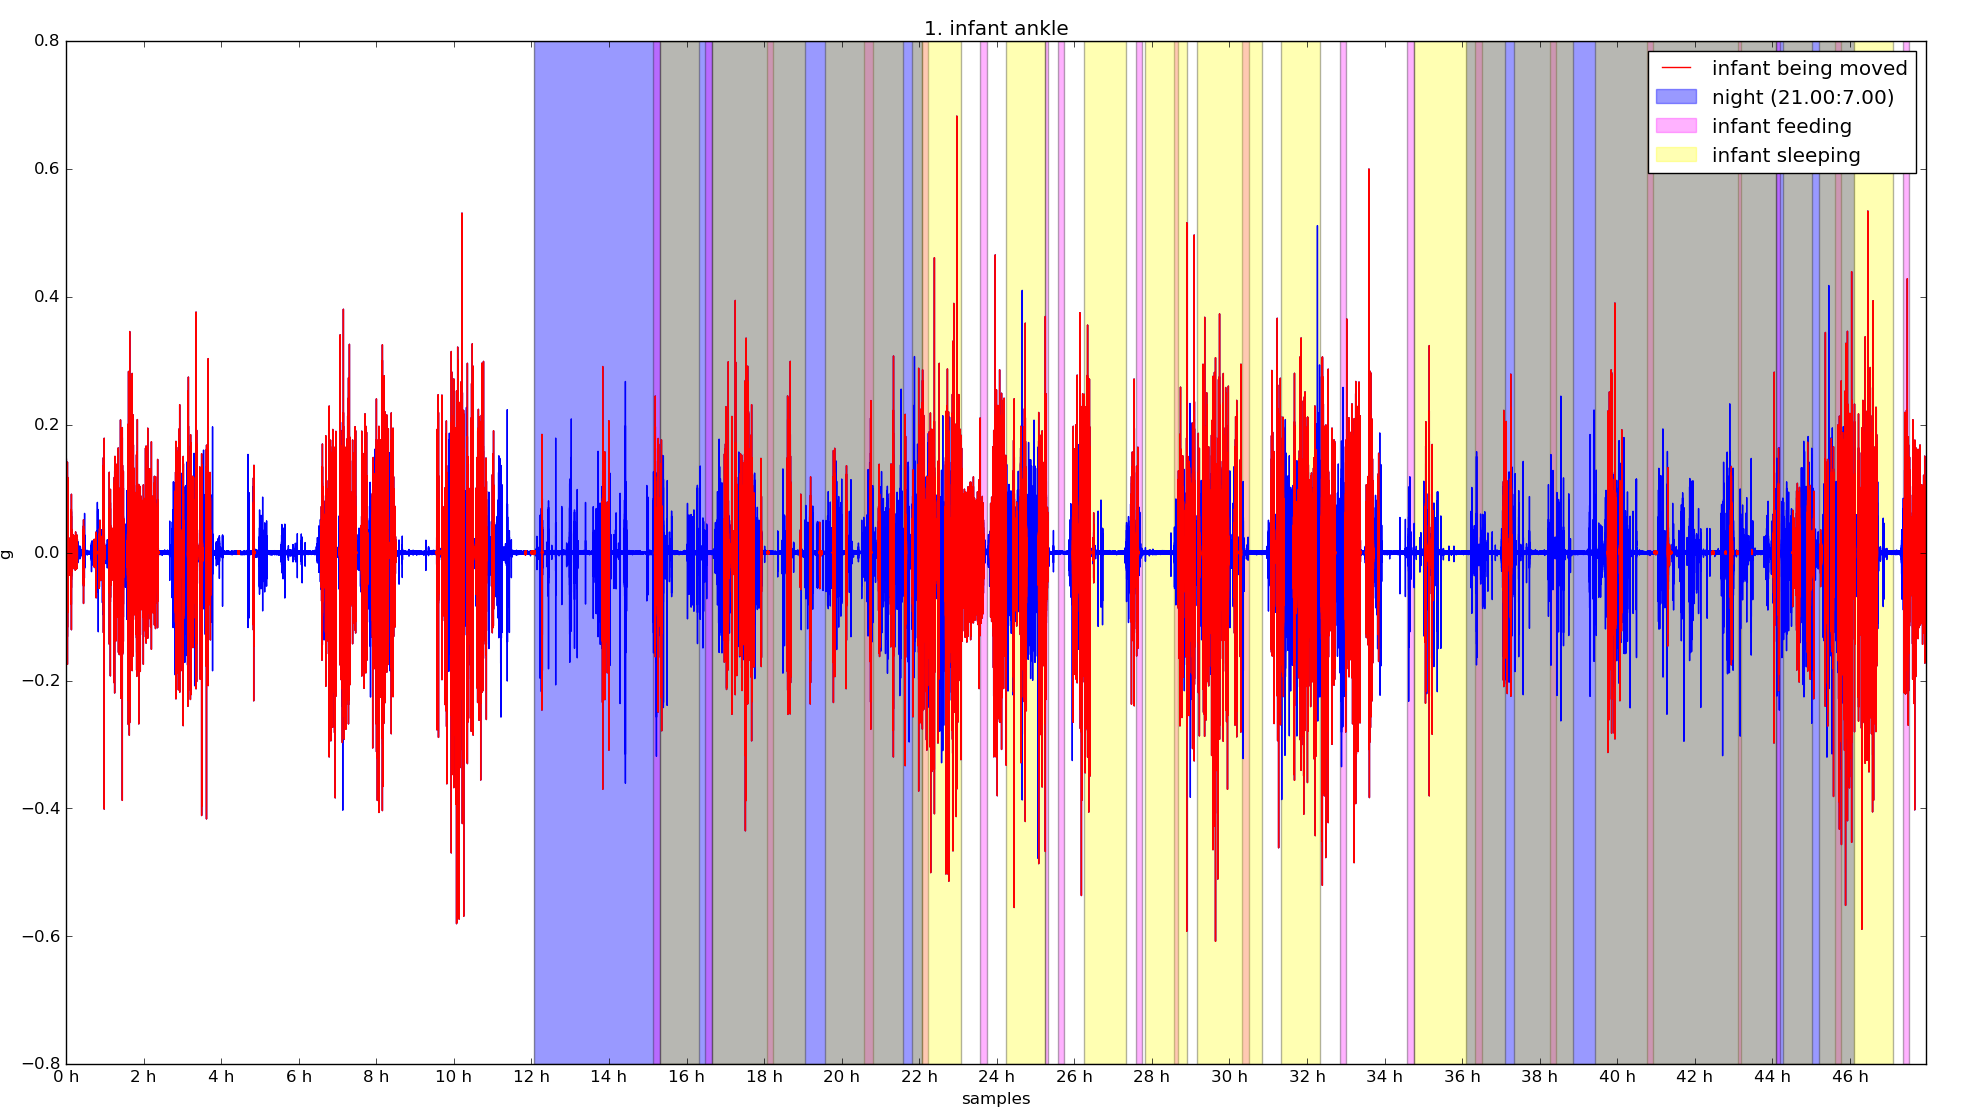
\includegraphics[width=15cm, height=6cm]{1moved.png}
\caption{The sleeping and feeding occurs in short blocks all through the experiment, night time is less expressed. }
\end{figure}

\begin{figure}[h]
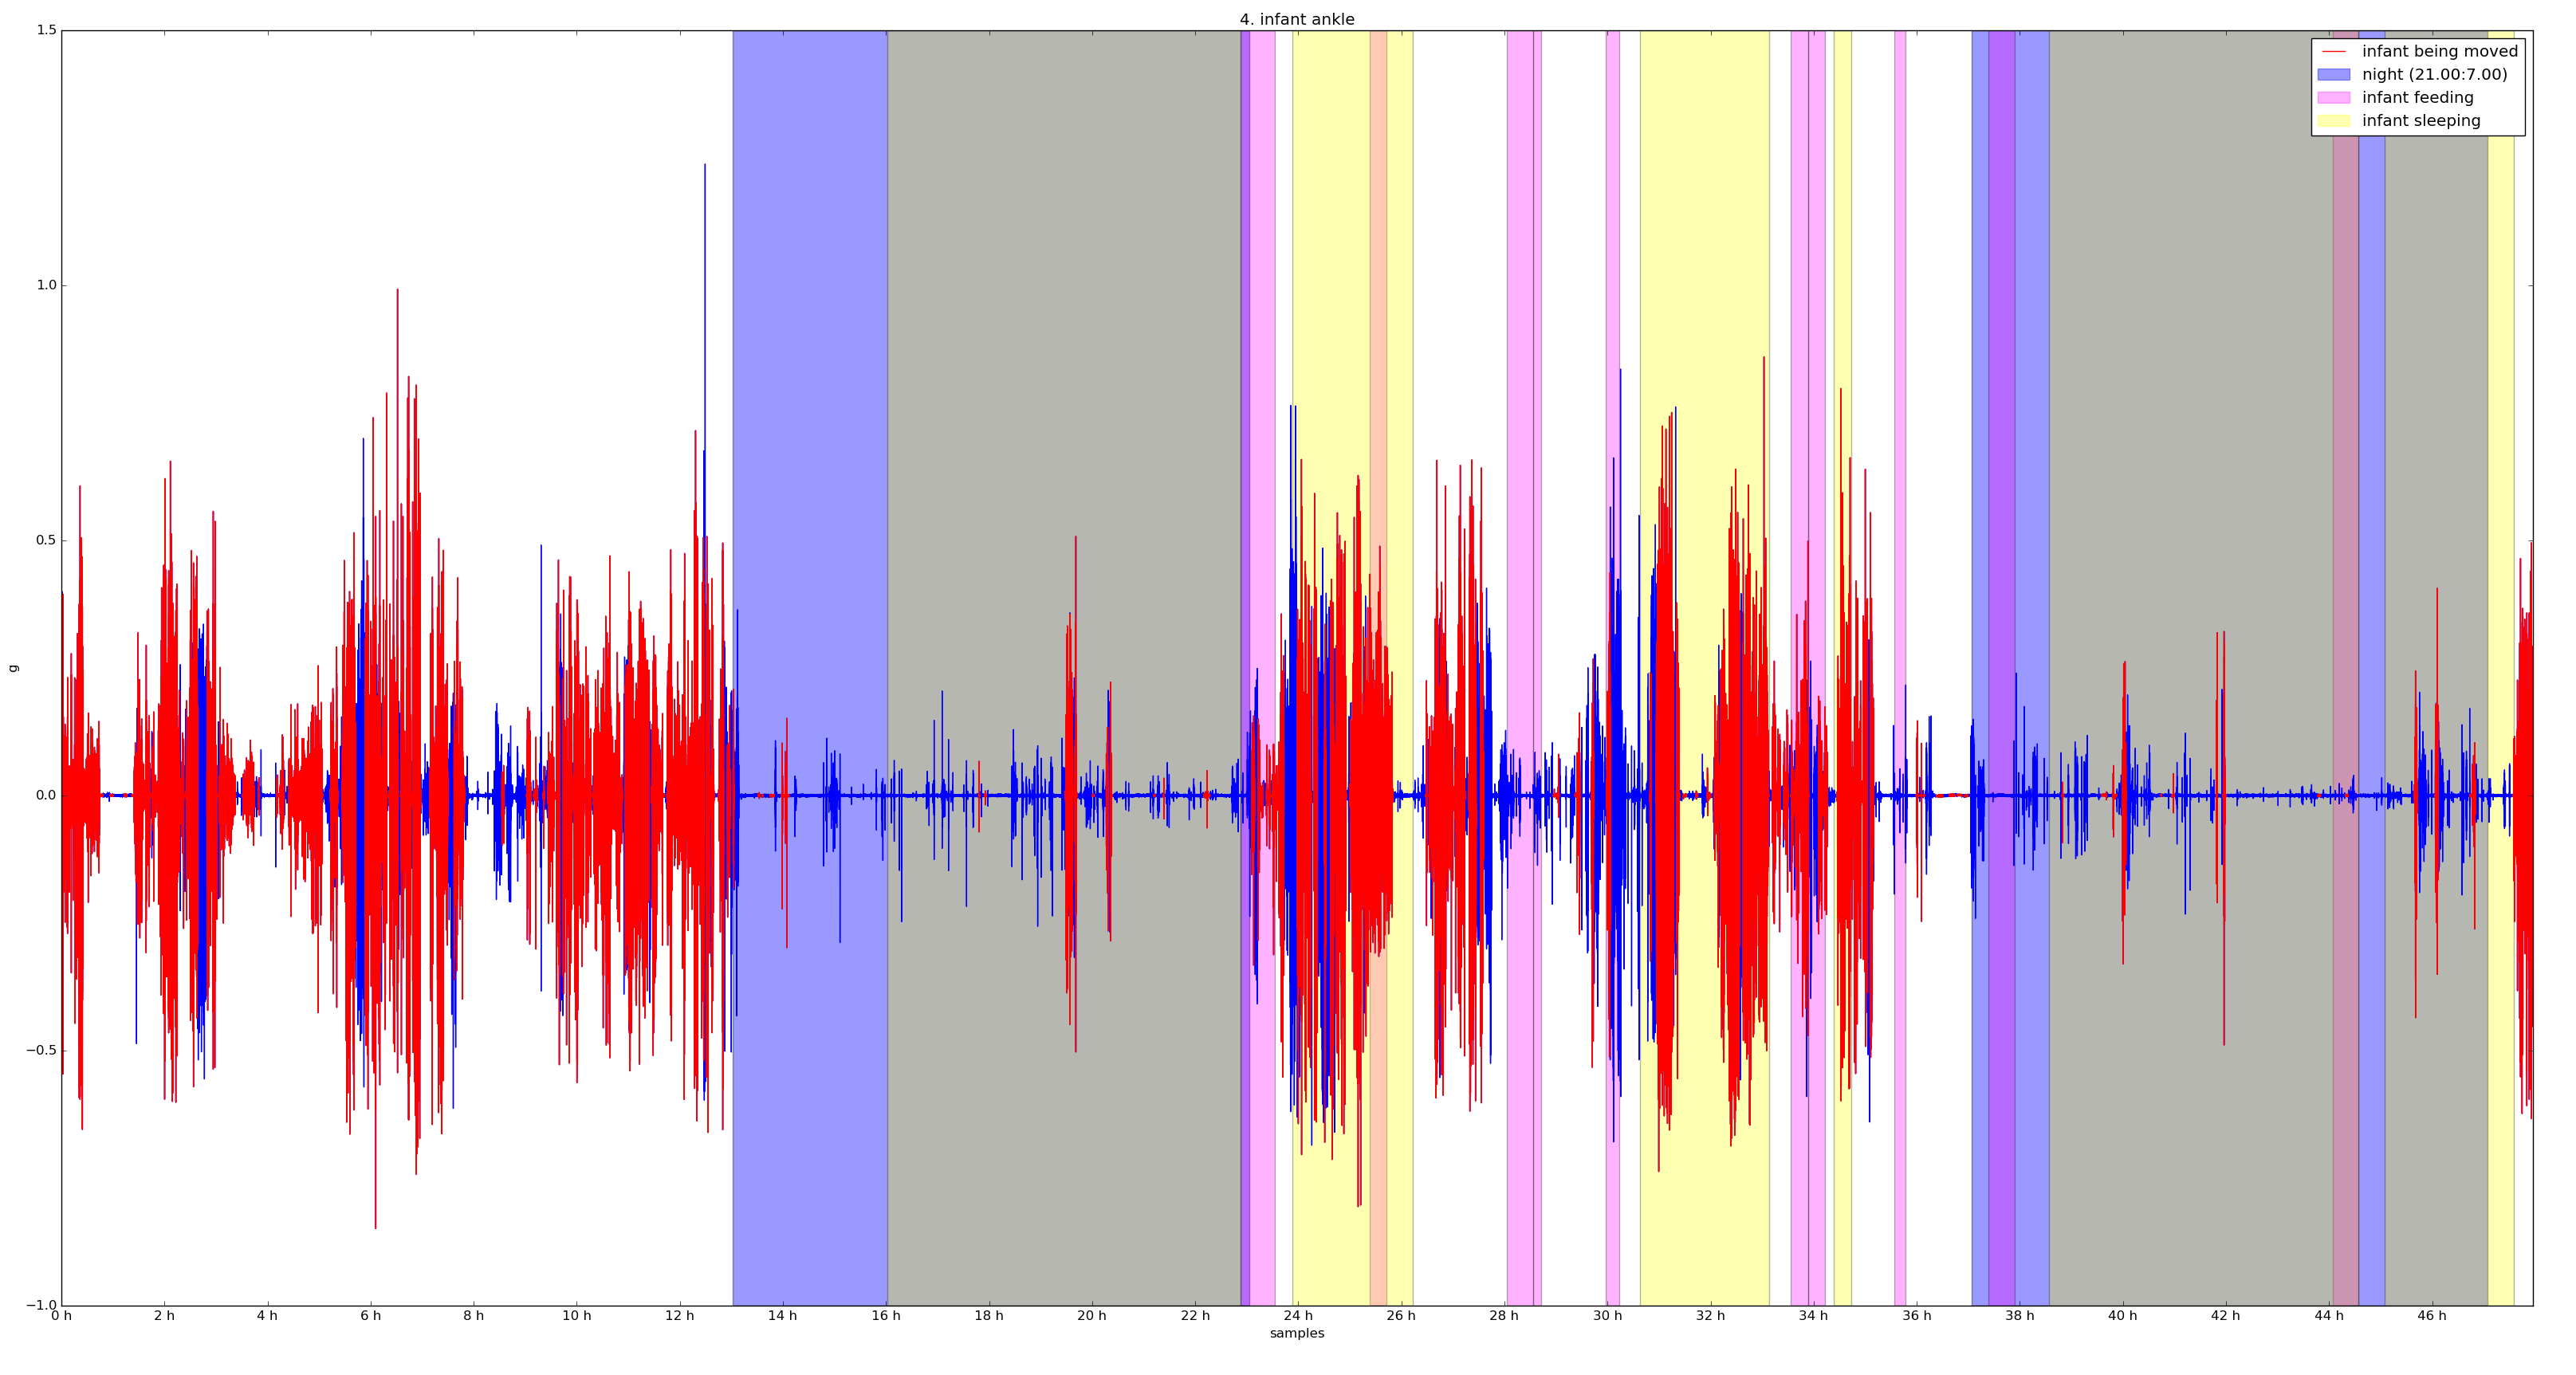
\includegraphics[width=15cm, height=7cm]{4moved.png}
\caption{The sleeping and feeding occurs in larger blocks, night time is more expressed with clearly less \textit{infant being moved} blocks.}
\end{figure}
Evidently, the diaries are not precise enough to validate the detection and correction of the contributing accelerations. Nevertheless, the extracted proportion of PA can be compared against the sleeping and awake blocks, in order to compare the amount of PA during sleeping and during awake time. Table 3 presents the proportion of time the extracted PA occurred while infant awake time.\\
\begin{table}[h]
\centering
\begin{tabular}{|l|l|l|l|}
\hline
     & approach C & approach D & approach E \\ \hline
mean & 48.12\%    & 45.87\%    & 35.48\%    \\ \hline
min  & 30.60\%    & 23.98\%    & 14.21\%    \\ \hline
max  & 61.51\%    & 61.13\%    & 59.02\%    \\ \hline
SD   & 10.83\%    & 09.02\%    & 12.71\%    \\ \hline
\end{tabular}
\caption{Proportions of PA occurring while infant awake, after different approaches.}
\end{table}
\\
In all approaches, the average proportion of PA occurring while infant sleeping is larger then expected, although the SD of the proportions is again very high, as is the span between the minimum and maximum and most importantly, the outcomes might not be accurate, since as previously mentioned, normalization with the total sleeping and awake time should had been done. Nevertheless, it is an approximation of the differences between the approaches. After approach \textbf{E} the average proportion of PA occurring during infant awake time is the smallest, implying as if the infant is more active during sleep. Considering previous observations regarding approach \textbf{E}, there is a chance that by removing all the blocks of \textit{infant being moved}, the extraction of PA becomes too limited on the time the infant was sleeping, example in Figure 26.
 \begin{figure}[h!]
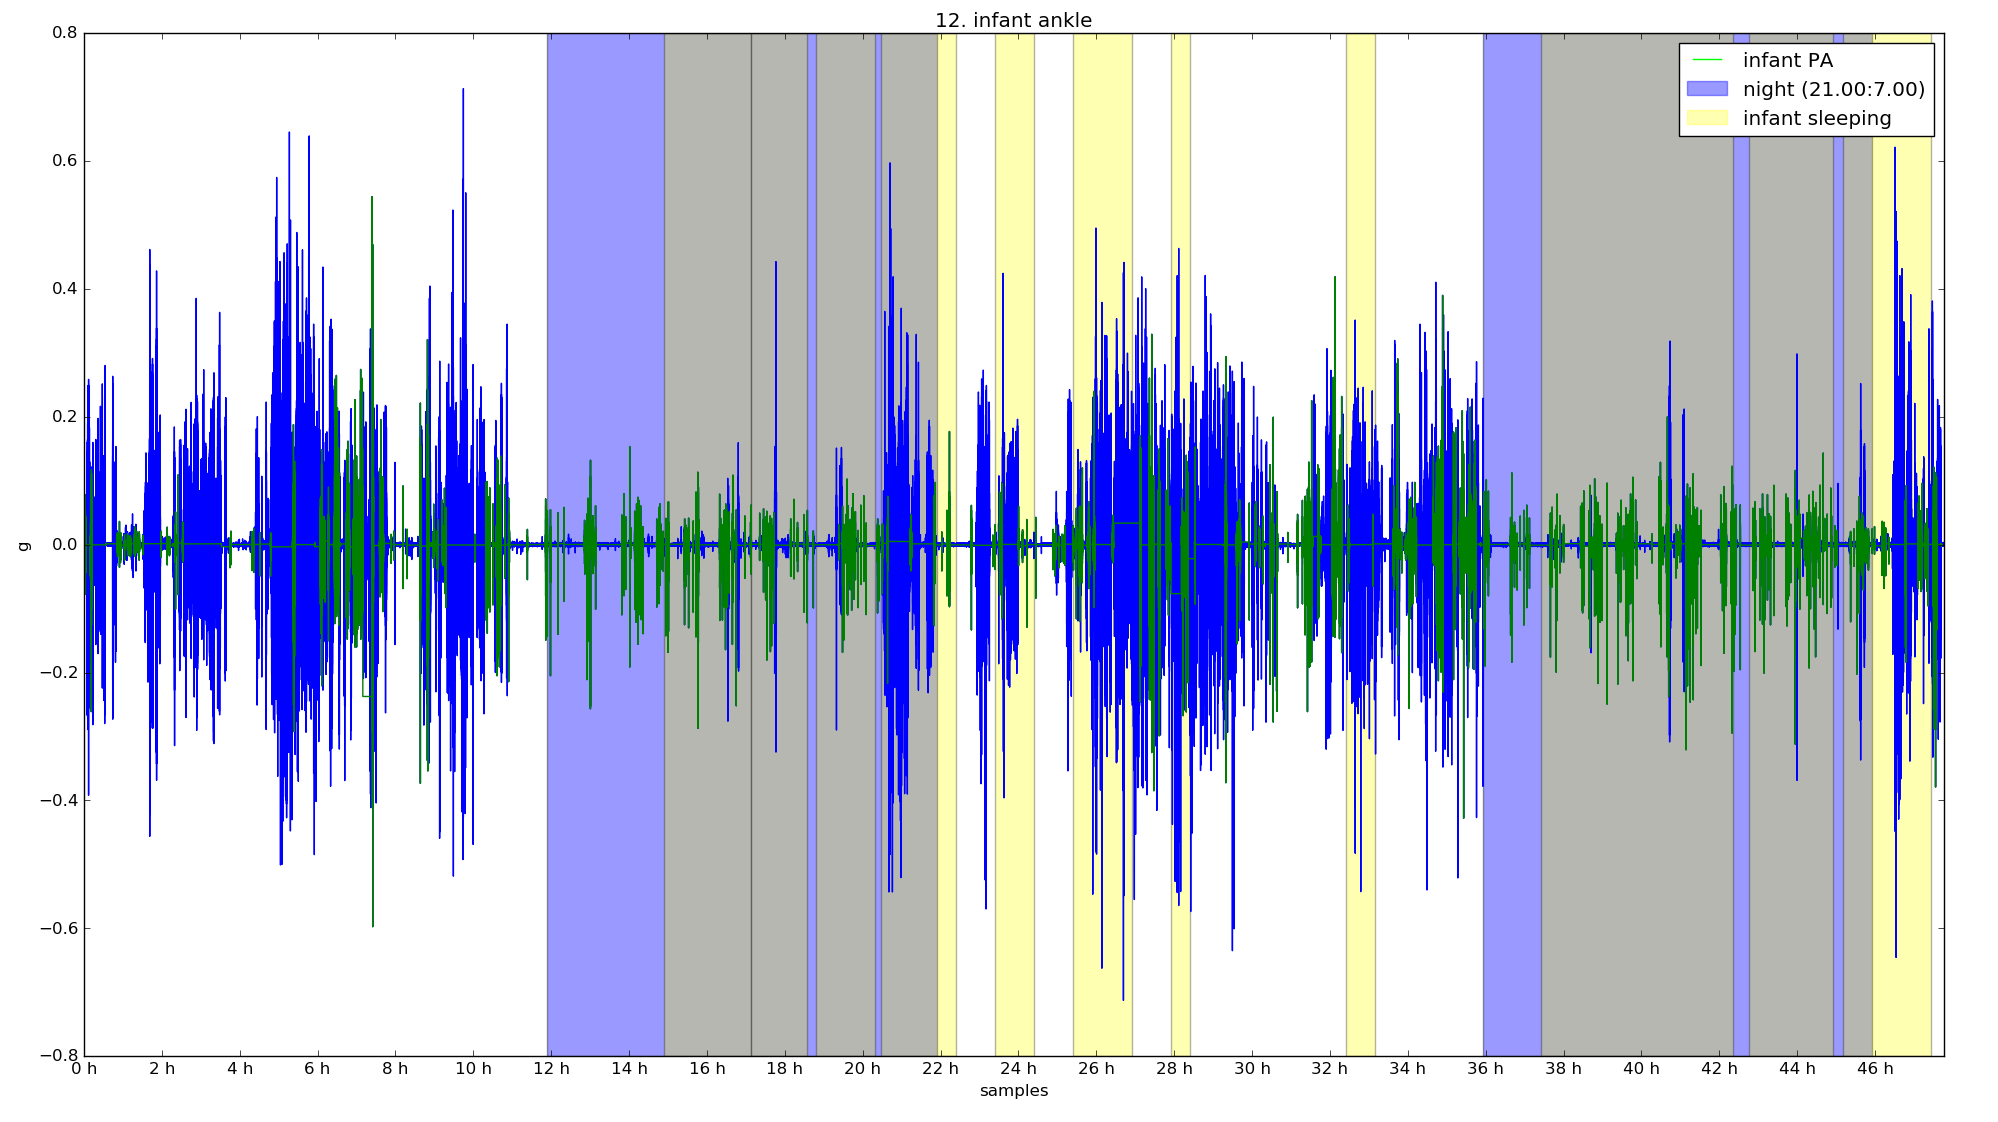
\includegraphics[width=15cm, height=7cm]{12PA.png}
\caption{Example of the extracted PA along with the diary noted sleep and night time according to the absolute timestamp.}
\end{figure}
\\Overall, the validation against the diaries did not provide the desired and planed validation due to the amount of error present in the diaries and introduced with digitization as well as due to fact that the accelerometer measurement and diary notations overlapped only for two nights and one day, which is not sufficient and biased to \textit{sleeping} time. Another issue is the high variability between the subjects, which was also observed in the previous steps of analysis. This overall high variability present between the subjects, between the activities and between the monitors might be too high for the size of the dataset. For example, the diary noted, sleeping and feeding proportions had high variability between the subjects, example in Table 4, raising doubt if validation over 29 subjects for 33 hours is possible.
\begin{table}[h]
\centering
\begin{tabular}{|l|l|l|}
\hline
over all subjects & sleeping time & feeding time \\ \hline
mean              & 63.00\%       & 9.63\%       \\ \hline
min               & 38.99\%       & 3.30\%       \\ \hline
max               & 81.60\%       & 27.01\%      \\ \hline
SD                & 9.39\%        & 6.01\%       \\ \hline
\end{tabular}
\caption{Proportion of sleeping and feeding time overall subjects with a diary available.}
\end{table}
\\One could also question whether the detection of contributing accelerations is possible with the size of the dataset and the amount of variability. This is discussed in the next chapter.
}


\section{Closure}
\fontsize{11.25pt}{11.1pt}\selectfont {

\subsection{Discussion}
None of the approaches resulted in a validated PA variable and now the question is, how feasible it is to estimate infants PA based on 30 subjects, using accelerometers in 48 hours.
Table 5 gives examples of variability present in a dataset of 30 subjects.
\begin{table}[h]
\centering
\begin{tabular}{|p{1cm}|p{4cm}|p{4cm}|p{4cm}|}
\hline
     & mean over all ankle summary & mean SD of infant being moved blocks & mean of the proportion of smaller torso placed measurement \\ \hline
mean & 2.0993e-12 g                & 0.013 g                              & 52.9\%                                                     \\ \hline
min  & -0.313 g                    & 0.0103 g                             & 47.8\%                                                     \\ \hline
max  & 0.355 g                     & 0.183 g                              & 62.3\%                                                     \\ \hline
SD   & 0.011 g                     & 0.002 g                              & 0.02\%                                                     \\ \hline
\end{tabular}
\caption{Examples of variability in the dataset of 30 subjects.}
\end{table}
\\With such high variability, one should consider the statistical power/sample size of the analysis, which will nevertheless, still have to be better than the approaches in this project. Even if having an appropriately sized dataset with a reasonable chance of finding the underlying similarities between torso and ankle placed measurements, there are still issues present. For example, in approach \textbf{E}, one would need to estimate for how long would one have to measure infants PA to avoid interfering with the final results by extracting PA mainly during when infant is sleeping, if that is even possible. In approach \textbf{D}, a better method for assessing similarity is necessary, while it would also be necessary to consider the amount of similarity when the infant is not being moved by the caretaker. Here, it might be useful to examine, whether the two signals were more correlated within the apparent \textit{infant being moved} blocks, compared to the rest of the measurement. Unfortunately, for this project, this analysis is yet to be performed as the necessary time exceeds the one intended for this project.
\subsection{Conclusions}
The torso and ankle placed measurements exhibit a substantial amount of similarity on a large scale, which implies contributing accelerations due to infant being moved by the caretaker. The overall presence of similarity and the amount of blocks with highly increased SD of the torso placed measurement, correspond to the previous reports regarding confounding accelerations due to infants caretaker[1][5][6]. High variability present between the subjects and their characteristics is also observed as in previous reports. To enable a valid extraction of infants PA, the contributing accelerations need to be removed. Based on the approaches developed and explored in this project, one has to consider:
\begin{itemize}
\item There is a substantial amount of difference between the torso and ankle placed measurements on a local scale, therefor a good enough summary of the measurement has to be derived,
\item The torso placed measurement is not necessary smaller then the ankle placed one, so any kind of subtracting might result in impaired further analysis,
\item Extracting signal similarities could be a potentially good approach to correct contributing accelerations,
\item Removing all the apparent blocks of \textit{infant being moved} might interfere with the extraction of PA,
\item With high overall variability, sample size must be considered
\item To obtain appropriate and valid means of validation.
\end{itemize}

}
%----------------------------------------------------------------------------------------
%	REFERENCE LIST
%----------------------------------------------------------------------------------------
\newpage
\begin{thebibliography}{99} 

\bibitem[1]{ref1}
Worobey J, Vetrini NR, Rozo EM (2009) Mechanical measurement of infant activity: A cautionary note.
\newblock \textit{Infant Behav Dev} 32(2):167-72.
\bibitem[2]{ref2}
van Hees VT, Renstrom F, Wright A, Gradmark A, Catt M, et al (2011) Estimation of Daily Energy Expenditure in Pregnant and Non-Pregnant Women
Using a Wrist-Worn Tri-Axial Accelerometer. PLoS ONE 6(7): e22922. doi:10.1371/journal.pone.0022922
\bibitem[3]{ref3}
van Hees VT, Gorzelniak L, Dean Leon EC, Eder M, Pias M, et al. (2013) Separating Movement and Gravity Components in an Acceleration Signal and
Implications for the Assessment of Human Daily Physical Activity. PLoS ONE 8(4): e61691. doi:10.1371/journal.pone.0061691
\bibitem[4]{ref4}
P.\ H.\ C.\ Eilers (2003) A Perfect Smoother.
\textit{Anal. Chem.} 2003, 75, 3631-3636
\bibitem[5]{ref5}
Spencer C, Taylor R, Gray A, Dale K, Taylor B. (2012) Use of accelerometer to measure physical activity in
6 month old infants. \textit{Australia New Zealand Obesity Society Conference} (ANZOS) 2012: \textit{For our
children's children}. Auckland, New Zealand.
\bibitem[6]{ref6}
Christine Moir (2014) Physical activity in infancy: assessment of an intervention to increase physical activity in infants.\\
A thesis submitted for the degree of Doctor of Philosophy at the University of Otago, Dunedin, New Zealand
\bibitem[7]{ref7}
Zhang S, Murray P, Zillmer R, Eston RG, Catt M, Rowlands AV (2012) Activity classification using the GENEA: optimum sampling frequency and number of axes.
\newblock \textit{Med Sci Sports Exerc.};44(11):2228-34. doi: 10.1249/MSS.0b013e31825e19fd.
\bibitem[8]{ref8}
Phan DH, Bonnet S, Guillemaud R, Castelli E, Pham Thi NY (2008) Estimation of respiratory waveform and heart rate using an accelerometer. Conf Proc IEEE
Eng Med Biol Soc 2008: 4916-4919.
\bibitem[9]{ref9}
Di Lena P, Margara L (2010) Optimal global alignment of signals by maximization of Pearson correlation. 
\textit{Information Processing Letters 110 (2010)}: 679-686
\bibitem[10]{ref10}
https://en.wikipedia.org/wiki/Pearson\_product-moment\_correlation\_coefficien-
t\#Using\_a\_permutation\_test
\bibitem[11]{ref11}
Perlin M, Bustamante DM (2014) A Robust Quantitative Comparison Criterion of Two Signals based 
on the Sobolev Norm of Their Difference.\\
arXiv:1412.6977 [physics.flu-dyn]
\bibitem[12]{ref12}
R.E.A. van Emmerik, S.W. Ducharme, A.C. Amado, J. Hamill (2016) Comparing dynamical systems concepts and techniques for biomechanical analysis\\ 
J Sport Health Sci, 5 (2016), pp. 3-13
\bibitem[13]{ref13}
Mudelsee M (2003) Estimating Pearsons Correlation Coefficient With Bootstrap Confidence Interval From Serially
Dependent Time Series\\
Mathematical Geology, Vol. 35, No. 6
\bibitem[14]{ref14}
Angela C. Estampador \textit{et al.} (2014), Infant Body Composition and Adipokine Concentrations in Relation to Maternal Gestational Weight Gain,
\newblock \textit{Diabetes Care, Volume 37}
\bibitem[15]{ref15}
Angela C Estampador, Paul W Franks (2014), Genetic and epigenetic catalysts in early-life programming of adult cardiometabolic disorders, Dovepress: \\http://dx.doi.org/10.2147/DMSO.S51433
\bibitem[16]{ref16}
Jeremy Pomeroy, Frida Renstrom, Paul W Franks \textit{et al.}, (2013) Maternal Physical Activity and Insulin Action in Pregnancy and Their Relationships With Infant Body Composition, Diabetes Care 36:267-269, DOI: 10.2337/dc12-0885
\end{thebibliography}
%----------------------------------------------------------------------------------------
\\
\\
\\
\\
\\
\\
\\
\\
\\
\Large{\textbf{Supplements}}
\\
\\
\normalsize Example of a diary kept by the infants mother.
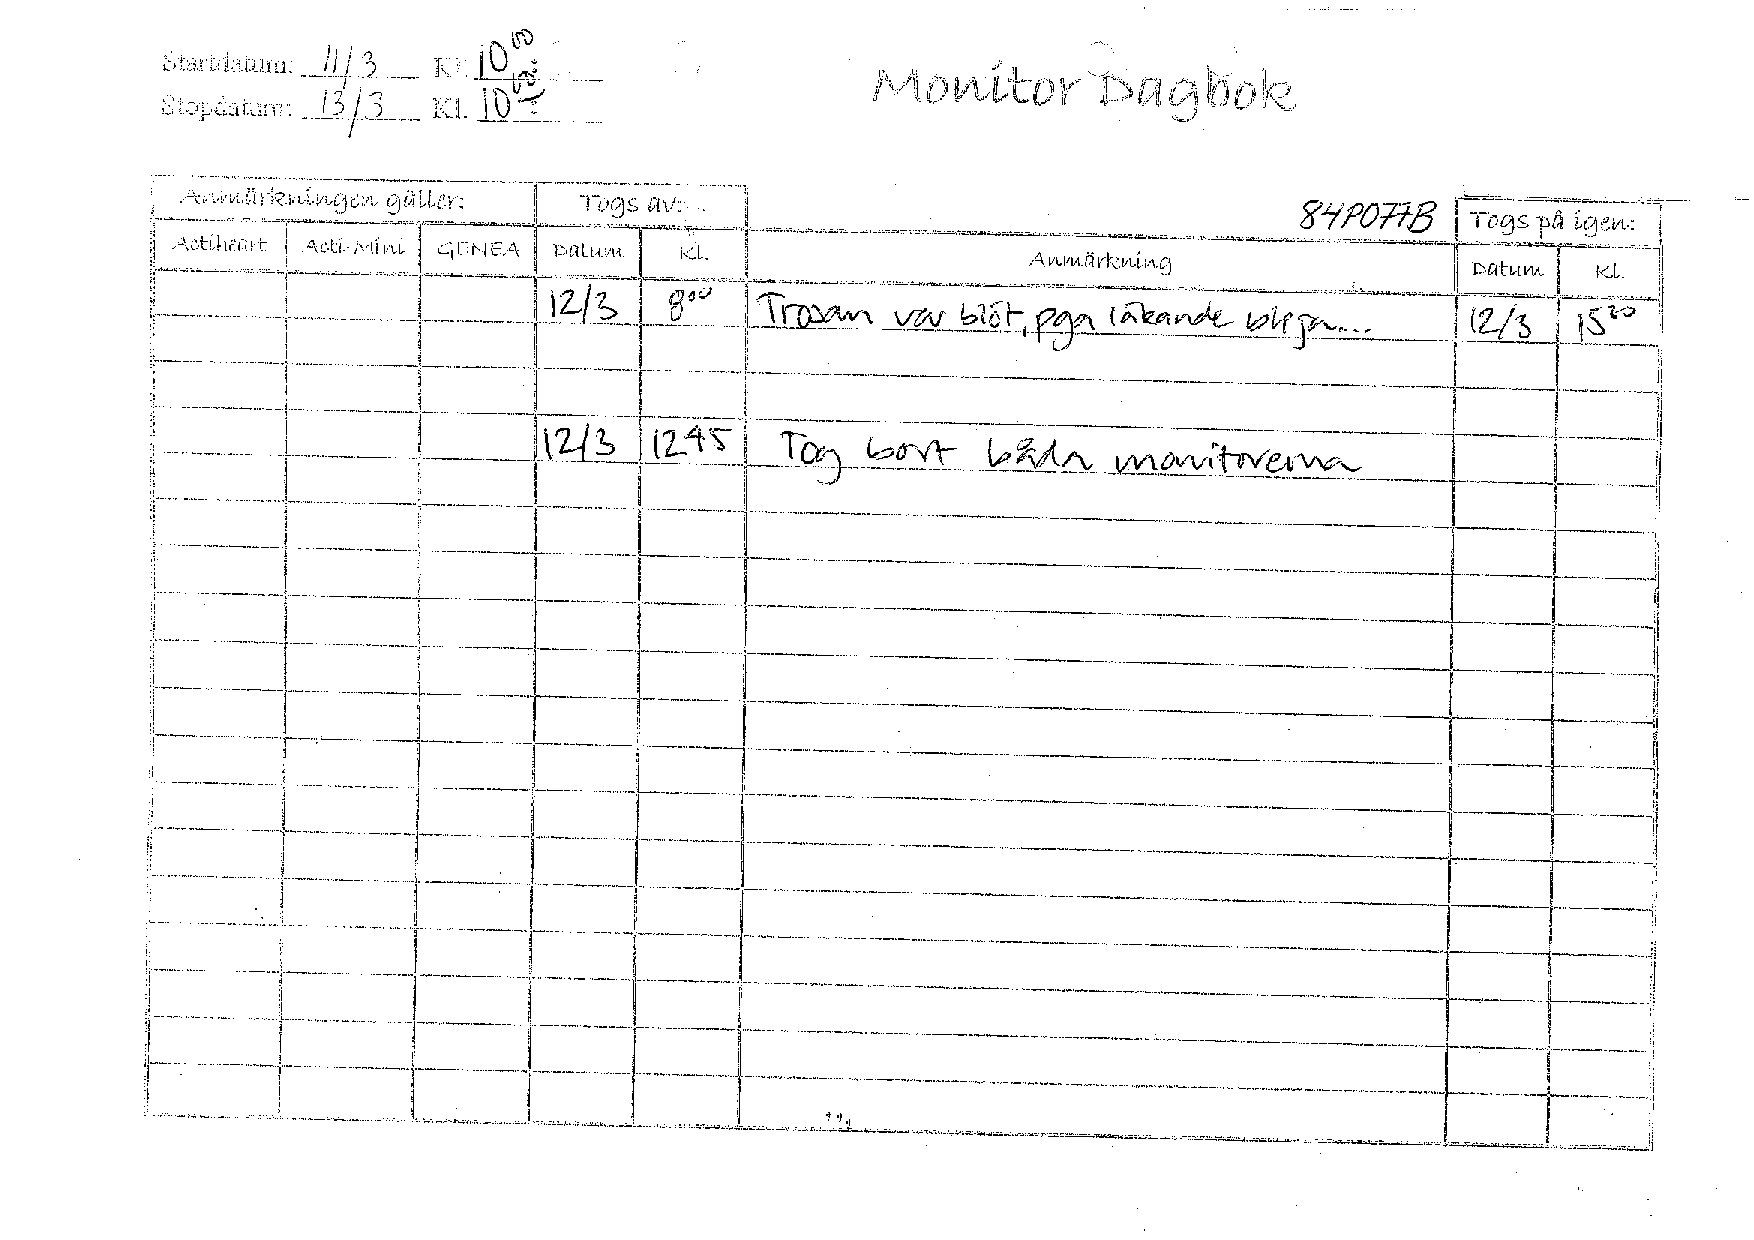
\includepdf[pages=-]{friendly_84P077.pdf}
\end{document}based
